% Options for packages loaded elsewhere
\PassOptionsToPackage{unicode}{hyperref}
\PassOptionsToPackage{hyphens}{url}
%
\documentclass[
]{article}
\usepackage{lmodern}
\usepackage{amssymb,amsmath}
\usepackage{ifxetex,ifluatex}
\ifnum 0\ifxetex 1\fi\ifluatex 1\fi=0 % if pdftex
  \usepackage[T1]{fontenc}
  \usepackage[utf8]{inputenc}
  \usepackage{textcomp} % provide euro and other symbols
\else % if luatex or xetex
  \usepackage{unicode-math}
  \defaultfontfeatures{Scale=MatchLowercase}
  \defaultfontfeatures[\rmfamily]{Ligatures=TeX,Scale=1}
\fi
% Use upquote if available, for straight quotes in verbatim environments
\IfFileExists{upquote.sty}{\usepackage{upquote}}{}
\IfFileExists{microtype.sty}{% use microtype if available
  \usepackage[]{microtype}
  \UseMicrotypeSet[protrusion]{basicmath} % disable protrusion for tt fonts
}{}
\makeatletter
\@ifundefined{KOMAClassName}{% if non-KOMA class
  \IfFileExists{parskip.sty}{%
    \usepackage{parskip}
  }{% else
    \setlength{\parindent}{0pt}
    \setlength{\parskip}{6pt plus 2pt minus 1pt}}
}{% if KOMA class
  \KOMAoptions{parskip=half}}
\makeatother
\usepackage{xcolor}
\IfFileExists{xurl.sty}{\usepackage{xurl}}{} % add URL line breaks if available
\IfFileExists{bookmark.sty}{\usepackage{bookmark}}{\usepackage{hyperref}}
\hypersetup{
  pdftitle={The Science and Art of Data},
  pdfauthor={Hui Lin and Ming Li},
  hidelinks,
  pdfcreator={LaTeX via pandoc}}
\urlstyle{same} % disable monospaced font for URLs
\usepackage[margin=1in]{geometry}
\usepackage{color}
\usepackage{fancyvrb}
\newcommand{\VerbBar}{|}
\newcommand{\VERB}{\Verb[commandchars=\\\{\}]}
\DefineVerbatimEnvironment{Highlighting}{Verbatim}{commandchars=\\\{\}}
% Add ',fontsize=\small' for more characters per line
\usepackage{framed}
\definecolor{shadecolor}{RGB}{248,248,248}
\newenvironment{Shaded}{\begin{snugshade}}{\end{snugshade}}
\newcommand{\AlertTok}[1]{\textcolor[rgb]{0.94,0.16,0.16}{#1}}
\newcommand{\AnnotationTok}[1]{\textcolor[rgb]{0.56,0.35,0.01}{\textbf{\textit{#1}}}}
\newcommand{\AttributeTok}[1]{\textcolor[rgb]{0.77,0.63,0.00}{#1}}
\newcommand{\BaseNTok}[1]{\textcolor[rgb]{0.00,0.00,0.81}{#1}}
\newcommand{\BuiltInTok}[1]{#1}
\newcommand{\CharTok}[1]{\textcolor[rgb]{0.31,0.60,0.02}{#1}}
\newcommand{\CommentTok}[1]{\textcolor[rgb]{0.56,0.35,0.01}{\textit{#1}}}
\newcommand{\CommentVarTok}[1]{\textcolor[rgb]{0.56,0.35,0.01}{\textbf{\textit{#1}}}}
\newcommand{\ConstantTok}[1]{\textcolor[rgb]{0.00,0.00,0.00}{#1}}
\newcommand{\ControlFlowTok}[1]{\textcolor[rgb]{0.13,0.29,0.53}{\textbf{#1}}}
\newcommand{\DataTypeTok}[1]{\textcolor[rgb]{0.13,0.29,0.53}{#1}}
\newcommand{\DecValTok}[1]{\textcolor[rgb]{0.00,0.00,0.81}{#1}}
\newcommand{\DocumentationTok}[1]{\textcolor[rgb]{0.56,0.35,0.01}{\textbf{\textit{#1}}}}
\newcommand{\ErrorTok}[1]{\textcolor[rgb]{0.64,0.00,0.00}{\textbf{#1}}}
\newcommand{\ExtensionTok}[1]{#1}
\newcommand{\FloatTok}[1]{\textcolor[rgb]{0.00,0.00,0.81}{#1}}
\newcommand{\FunctionTok}[1]{\textcolor[rgb]{0.00,0.00,0.00}{#1}}
\newcommand{\ImportTok}[1]{#1}
\newcommand{\InformationTok}[1]{\textcolor[rgb]{0.56,0.35,0.01}{\textbf{\textit{#1}}}}
\newcommand{\KeywordTok}[1]{\textcolor[rgb]{0.13,0.29,0.53}{\textbf{#1}}}
\newcommand{\NormalTok}[1]{#1}
\newcommand{\OperatorTok}[1]{\textcolor[rgb]{0.81,0.36,0.00}{\textbf{#1}}}
\newcommand{\OtherTok}[1]{\textcolor[rgb]{0.56,0.35,0.01}{#1}}
\newcommand{\PreprocessorTok}[1]{\textcolor[rgb]{0.56,0.35,0.01}{\textit{#1}}}
\newcommand{\RegionMarkerTok}[1]{#1}
\newcommand{\SpecialCharTok}[1]{\textcolor[rgb]{0.00,0.00,0.00}{#1}}
\newcommand{\SpecialStringTok}[1]{\textcolor[rgb]{0.31,0.60,0.02}{#1}}
\newcommand{\StringTok}[1]{\textcolor[rgb]{0.31,0.60,0.02}{#1}}
\newcommand{\VariableTok}[1]{\textcolor[rgb]{0.00,0.00,0.00}{#1}}
\newcommand{\VerbatimStringTok}[1]{\textcolor[rgb]{0.31,0.60,0.02}{#1}}
\newcommand{\WarningTok}[1]{\textcolor[rgb]{0.56,0.35,0.01}{\textbf{\textit{#1}}}}
\usepackage{graphicx,grffile}
\makeatletter
\def\maxwidth{\ifdim\Gin@nat@width>\linewidth\linewidth\else\Gin@nat@width\fi}
\def\maxheight{\ifdim\Gin@nat@height>\textheight\textheight\else\Gin@nat@height\fi}
\makeatother
% Scale images if necessary, so that they will not overflow the page
% margins by default, and it is still possible to overwrite the defaults
% using explicit options in \includegraphics[width, height, ...]{}
\setkeys{Gin}{width=\maxwidth,height=\maxheight,keepaspectratio}
% Set default figure placement to htbp
\makeatletter
\def\fps@figure{htbp}
\makeatother
\usepackage[normalem]{ulem}
% Avoid problems with \sout in headers with hyperref
\pdfstringdefDisableCommands{\renewcommand{\sout}{}}
\setlength{\emergencystretch}{3em} % prevent overfull lines
\providecommand{\tightlist}{%
  \setlength{\itemsep}{0pt}\setlength{\parskip}{0pt}}
\setcounter{secnumdepth}{-\maxdimen} % remove section numbering

\title{The Science and Art of Data}
\author{Hui Lin and Ming Li}
\date{2020-05-18}

\begin{document}
\maketitle

\hypertarget{learning-outcomes}{%
\section{LEARNING OUTCOMES}\label{learning-outcomes}}

After taking the CE course, participants will:

\begin{itemize}
\item
  Understand what data scientists ``in the wild'' are doing.
\item
  Understand data science is the process of defining the problem with
  business knowledge, gathering needed data from various sources,
  developing models, extracting insight and recommend actions.
\item
  Get familiar with the cloud-based big data platform
  (Hadoop/Hive/Spark/GPU etc.) that are widely used in the development
  and production setting for industry and know how to transit from
  academic environment to enterprise environment quickly.
\item
  Get familiar with data extraction, transformation and load from
  various database systems such that participates can be self-sufficient
  to get needed data in the enterprise environment.
\item
  Understand how to leverage interactive dashboard to present insight
  and results and communicate efficiently with business partners and
  customers
\item
  Learn how to encode a real problem to a data science problem, search
  for the right data, preprocess data and deploy of analytical results
  through a case study
\item
  Get familiar with how to achieve high-performance computing for
  standard statistical procedures with big data infrastructure 
\end{itemize}

\hypertarget{the-art-of-data-science}{%
\section{The art of data science}\label{the-art-of-data-science}}

Data science and data scientist have become buzz words. Allow me to
reiterate what you may have already heard a million times in the media:
\textbf{data scientists are in demand and demand continues to grow}. A
study by the McKinsey Global Institute concludes,

\begin{quote}
``a shortage of the analytical and managerial talent necessary to make
the most of Big Data is a significant and pressing challenge (for the
U.S.).''
\end{quote}

You may expect that statisticians and graduate students from traditional
statistics departments are great data scientist candidates. But the
situation is that the majority of current data scientists do not have a
statistical background. As David Donoho pointed out:

\begin{quote}
``statistics is being marginalized here; the implicit message is that
statistics is a part of what goes on in data science but not a very big
part.'' ( from
``\href{http://pages.cs.wisc.edu/~anhai/courses/784-fall15/50YearsDataScience.pdf}{50
years of Data Science}'').
\end{quote}

What is wrong? The activities that preoccupied statistics over centuries
are now in the limelight, but those activities are claimed to belong to
a new discipline and are practiced by professionals from various
backgrounds. Various professional statistics organizations are reacting
to this confusing situation. (Page 5-7, ``50 Years of Data Science'')
From those discussions, Donoho summarizes the main recurring ``Memes''
about data sciences:

\begin{enumerate}
\def\labelenumi{\arabic{enumi}.}
\tightlist
\item
  The `Big Data' Meme
\item
  The `Skills' Meme
\item
  The `Jobs' Meme
\end{enumerate}

The first two are linked together which leads to statisticians' current
position on data science. I assume everyone has heard the 3V (volume,
variety and velocity) definition of big data. The media hasn't taken a
minute break from touting ``big'' data. Data science trainees now need
the skills to cope with such big data sets. What are those skills? You
may hear about: Hadoop, system using Map/Reduce to process large data
sets distributed across a cluster of computers. The new skills are for
dealing with organizational artifacts of large-scale cluster computing
but not for better solving the real problem. A lot of data on its own is
worthless. It isn't the size of the data that's important. It's what you
do with it. The big data skills that so many are touting today are not
skills for better solving the real problem of inference from data.

Some media think they sense the trends in hiring and government funding.
We are transiting to universal connectivity with a deluge of data
filling telecom servers. But these facts don't immediately create a
science. The statisticians have been laying the groundwork of data
science for at least 50 years. Today's data science is an enlargement of
traditional academic statistics rather than a brand new discipline.

Our goal is to help you enlarge your background to become a data
scientist in US enterprise environments. We will use case studies to
cover how to leverage big data distributed platforms (Hadoop / Hive /
Spark), data wrangling, modeling, dynamic reporting (R markdown) and
interactive dashboards (R-Shiny) to tackle real-world data science
problems. One typical skill gap for statisticians is data ETL
(extraction, transformation and load) in production environments, and we
will cover this topic as well. Data science is a combination of science
and art with data as the foundation. We will also cover the ``art'' part
to guide participants to learn soft skills to define data science
problems and to effectively communicate with business stakeholders. The
prerequisite knowledge is MS level education in statistics and entry
level knowledge of R-Studio.

\hypertarget{what-is-data-science}{%
\subsection{What is data science?}\label{what-is-data-science}}

This question is not new. When you tell people ``I am a data
scientist''. ``Ah, data scientist!'' Yes, who doesn't know that data
scientist is the sexist job in 21th century? If they ask further what is
data science and what exactly do data scientists do, it may effectively
kill the conversation.

Data Science doesn't come out of the blue. Its predecessor is data
analysis. Back in 1962, John Tukey wrote in ``The Future of Data
Analysis'':

\begin{quote}
For a long time I have thought I was a statistician, interested in
inferences from the particular to the general. But as I have watched
mathematical statistics evolve, I have had cause to wonder and to doubt.
\ldots{} All in all, I have come to feel that my central interest is in
data analysis, which I take to include, among other things: procedures
for analyzing data, techniques for interpreting the results of such
procedures, ways of planning the gathering of data to make its analysis
easier, more precise or more accurate, and all the machinery and results
of (mathematical) statistics which apply to analyzing data.
\end{quote}

It deeply shocked his academic readers. Aren't you supposed to present
something mathematically precise, such as definitions, theorems and
proofs? If we use one sentence to summarize what John said, it is:

\begin{quote}
data analysis is more than mathematics.
\end{quote}

In September 2015, the University of Michigan make plans to invest \$100
million over the next five years in a new
\href{http://www.ns.umich.edu/new/releases/23105-u-michigan-launches-100-million-data-science-initiative}{Data
Science Initiative} that will enhance opportunities for student and
faculty researchers across the university to tap into the enormous
potential of big data. UM Provost Martha Pollack said:

\begin{quote}
``Data science has become a fourth approach to scientific discovery, in
addition to experimentation, modeling and computation,\ldots{}''
\end{quote}

How does the Data Science Initiative define Data science? Their website
gives us an idea:

\begin{quote}
``This coupling of scientific discovery and practice involves the
collection, management, processing, analysis, visualization, and
interpretation of vast amounts of heterogeneous data associated with a
diverse array of scientific, translational, and interdisciplinary
applications.''
\end{quote}

With the data science hype picking up stream, many professionals changed
their titles to Data Scientist without any of the necessary
qualifications. But at that time, the data scientist title was not well
defined which lead to confusion in the market, obfuscation in resumes,
and exaggeration of skills. Here is a list of somewhat whimsical
definitions for a ``data scientist'':

\begin{itemize}
\tightlist
\item
  ``A data scientist is a data analyst who lives in California''
\item
  ``A data scientist is someone who is better at statistics than any
  software engineer and better at software engineering than any
  statistician.''
\item
  ``A data scientist is a statistician who lives in San Francisco.''
\item
  ``Data Science is statistics on a Mac.''
\end{itemize}

There is lots of confusion between Data Scientist, Statistician,
Business/Financial/Risk(etc) Analyst and BI professional due to the
obvious intersections among skillsets. We see data science as a
discipline to make sense of data. In order to make sense of data,
statistics is indispensable. But a data scientist also needs many other
skills.

In the obscenity case of Jacobellis v. Ohio (1964), Potter Stewart wrote
in his short concurrence that ``hard-core pornography'' was hard to
define, but that ``I know it when I see it.'' This applies to many
things including data science. It is hard to define but you know it when
you see it.

So instead of scratching my head to figure out a one sentence
definition, We are going to sketch the history of data science, what
kind of questions data science can answer, and describe the skills
required for being a data scientist. We hope this can give you a better
depiction of data science.

In the early 19th century when Legendre and Gauss came up the least
squares method for linear regression, only physicists would use it to
fit linear regression. Now, even non-technical people can fit linear
regressions using excel. In 1936 Fisher came up with linear discriminant
analysis. In the 1940s, we had another widely used model -- logistic
regression. In the 1970s, Nelder and Wedderburn formulated ``generalized
linear model (GLM)'' which:

\begin{quote}
``generalized linear regression by allowing the linear model to be
related to the response variable via a link function and by allowing the
magnitude of the variance of each measurement to be a function of its
predicted value.'' {[}from Wikipedia{]}
\end{quote}

By the end of the 1970s, there was a range of analytical models and most
of them were linear because computers were not powerful enough to fit
non-linear model until the 1980s.

In 1984 Breiman et al.~introduced classification and regression tree
(CART) which is one of the oldest and most utilized classification and
regression techniques. After that Ross Quinlan came up with more tree
algorithms such as ID3, C4.5 and C5.0. In the 1990s, ensemble techniques
(methods that combine many models' predictions) began to appear. Bagging
is a general approach that uses bootstrapping in conjunction with any
regression or classification model to construct an ensemble. Based on
the ensemble idea, Breiman came up with random forest in 2001. Later,
Yoav Freund and Robert Schapire came up with the AdaBoost.M1 algorithm.
Benefiting from the increasing availability of digitized information,
and the possibility to distribute that via the internet, the tool box
has been expanding fast. The applications include business, health,
biology, social science, politics etc.

John Tukey identified 4 forces driving data analysis (there was no
``data science'' then):

\begin{enumerate}
\def\labelenumi{\arabic{enumi}.}
\tightlist
\item
  The formal theories of math and statistics
\item
  Acceleration of developments in computers and display devices
\item
  The challenge, in many fields, of more and ever larger bodies of data
\item
  The emphasis on quantification in an ever wider variety of disciplines
\end{enumerate}

Tukey's 1962 list is surprisingly modern. Let's inspect those points in
today's context. There is always a time gap between a theory and its
application. We had the theories much earlier than application.
Fortunately, for the past 50 years statisticians have been laying the
theoretical groundwork for constructing ``data science'' today. The
development of computers enables us to calculate much faster and deliver
results in a friendly and intuitive way. The striking transition to the
internet of things generates vast amounts of commercial data. Industries
have also sensed the value of exploiting that data. Data science seems
certain to be a major preoccupation of commercial life in coming
decades. All the four forces John identified exist today and have been
driving data science.

\hypertarget{is-it-science-totally}{%
\subsection{Is it science? Totally?}\label{is-it-science-totally}}

Let's take one step back. What is science? Here is what John Tukey said:

\begin{quote}
There are diverse views as to what makes a science, but three
constituents will be judged essential by most, viz:\\
(a1) intellectual content,\\
(a2) organization in an understandable form,\\
(a3) reliance upon the test of experience as the ultimate standard of
validity
\end{quote}

The first one (a1) doesn't provide useful information. And (a2) can't
distinguish science from art very well. The last one is a key character
of science. The influential philosopher of science Karl Popper argued
that science advances by falsifying hypotheses. If science needs to be
falsifiable, then data science is not 100\% science. It is true that
there are some analytical results that can be validated (falsified)
through cross validation or comparing prediction with future outcomes.
But certainly not all of them. Even in the problem of prediction, we
can't validate predictions in the 2nd order chaotic systems.

We can't scientifically validate many unsupervised learning or
descriptive analysis, especially in the context of marketing. In that
sense, data science is a combination of science and art.\\
There is another definition of science from the famous computer
scientist Donald Knuth. He said in his legendary 1974 essay
\href{http://www.paulgraham.com/knuth.html}{Computer Programming as an
Art}:

\begin{quote}
``Science is knowledge which we understand so well that we can teach it
to a computer.''
\end{quote}

Computers are indispensable for data science. But can we teach computers
to do all the work data scientists do today? No.~So it is not totally
science. Computers can't communicate with stakeholders to transform a
real life problem to be data problem. Computers don't know which
questions can be answered through analytics. Computers don't know how to
explain the results to different audiences using different ways
according to their backgrounds. Computers are powerful in many ways but
certainly not all. Would a computer enter a `runaway reaction' of
self-improvement cycles so that it could surpass human in every way in
the future? Well, that is not a question we are trying to answer here.
If you are interested in the future of technology, there are some books
you can refer to. Ray Kurzweil (The Singularity Is Near), Yuval Noah
Harari (Homo Deus: A Brief History of Tomorrow) and Kevin Kelly (The
Inevitable). At the risk of being short-sighted, we will assume it won't
happen in foreseeable future.

To be simple I will still use data science in the rest of the book. But
it is important to realize that data science includes art.

\hypertarget{what-kind-of-questions-can-data-science-solve}{%
\subsection{What kind of questions can data science
solve?}\label{what-kind-of-questions-can-data-science-solve}}

\hypertarget{prerequisites}{%
\subsubsection{Prerequisites}\label{prerequisites}}

Data science is not a panacea, and data scientists are not magicians.
There are problems data science can't help. It is best to make a
judgment as early in the analytical cycle as possible. Tell your clients
honestly and clearly when you figure data analytics can't give the
answer they want. What kind of questions can data science solve? What
are the requirements for our question?

\begin{enumerate}
\def\labelenumi{\arabic{enumi}.}
\tightlist
\item
  Your question needs to be specific enough
\end{enumerate}

Look at two examples:

\begin{itemize}
\tightlist
\item
  Question 1: How can I increase product sales?
\item
  Question 2: Is the new promotional tool introduced at the beginning of
  this year boosting the annual sales of P1197 in Iowa and Wisconsin?
  (P1197 is an impressive corn seed product from DuPont Pioneer)
\end{itemize}

It is easy to see the difference between the two questions. Question 1
is a grammatically correct question, but it is proper for data analysis
to answer. Why? It is too general. What is the response variable here?
Product sales? Which product? Is it annual sales or monthly sales? What
are the candidate predictors? You nearly can't get any useful
information from the questions. In contrast, question 2 is much more
specific. From the analysis point of view, the response variable is
clearly ``annual sales of P1197 in Iowa and Wisconsin''. Even we don't
know all the predictors, but the variable of interest is ``the new
promotional tool introduced early this year.'' We want to study the
impact of the promotion on the sales. You can start from there and move
on to figure out other variables need to include in the model by further
communication.

As a data scientist, you may start with something general and unspecific
like question 1 and eventually get to question 2. Effective
communication and in-depth domain knowledge about the business problem
are essential to convert a general business question into a solvable
analytical problem. Domain knowledge helps data scientist communicate
with the language the other people can understand and obtain the
required information.

However, defining the question and variables involved don't guarantee
that you can answer it. I have encountered a well-defined supply chain
problem. My client asked about the stock needed for a product in a
particular area. Why can not this question be answered? I did fit a
Multivariate Adaptive Regression Spline (MARS) model and thought I found
a reasonable solution. But it turned out later that the data they gave
me was inaccurate. In some areas, only estimates of past supply figures
were available. The lesson lends itself to the next point.

\begin{enumerate}
\def\labelenumi{\arabic{enumi}.}
\setcounter{enumi}{1}
\tightlist
\item
  You need to have sound and relevant data
\end{enumerate}

One cannot make a silk purse out of a sow's ear. Data scientists need
data, sound and relevant data. The supply problem is a case in point.
There was relevant data, but not sound. All the later analytics based on
that data was a building on sand. Of course, data nearly almost have
noise, but it has to be in a certain range. Generally speaking, the
accuracy requirement for the independent variables of interest and
response variable is higher than others. In question 2, it is data
related to the ``new promotion'' and ``sales of P1197''.

The data has to be helpful for the question. If you want to predict
which product consumers are most likely to buy in the next three months,
you need to have historical purchasing data: the last buying time, the
amount of invoice, coupons and so on. Information about customers'
credit card number, ID number, the email address is not going to help.

Often the quality of the data is more important than the quantity, but
the quantity can not be overlooked. In the premise of guaranteeing
quality, usually the more data, the better. If you have a specific and
reasonable question, also sound and relevant data, then congratulations,
you can start playing data science!

\hypertarget{problem-type}{%
\subsubsection{Problem type}\label{problem-type}}

Many of the data science books classify the various models from a
technical point of view. Such as supervised vs.~unsupervised models,
linear vs.~nonlinear models, parametric models vs.~non-parametric
models, and so on. Here we will continue on ``problem-oriented'' track.
We first introduce different groups of real problems and then present
which models can be used to answer the corresponding category of
questions.

\begin{enumerate}
\def\labelenumi{\arabic{enumi}.}
\tightlist
\item
  Comparison
\end{enumerate}

The first common problem is to compare different groups. Such as: Is A
better in some way than B? Or more comparisons: Is there any difference
among A, B, C in a certain aspect? Here are some examples:

\begin{itemize}
\tightlist
\item
  Are the purchasing amounts different between consumers receiving
  coupons and those without coupons?
\item
  Are males more inclined to buy our products than females?
\item
  Are there any differences in customer satisfaction in different
  business districts?
\item
  Do the mice receiving a drug have a faster weight gain than the
  control group?
\item
  Do soybeans carrying a particular gene contain more oil than the
  control group?
\end{itemize}

For those problems, it is usually to start exploring from the summary
statistics and visualization by groups. After a preliminary
visualization, you can test the differences between treatment and
control group statistically. The commonly used statistical tests are
chi-square test, t-test, and ANOVA. There are also methods using
Bayesian methods. In biology industry, such as new drug development,
crop breeding, mixed effect models are the dominant technique.

\begin{enumerate}
\def\labelenumi{\arabic{enumi}.}
\setcounter{enumi}{1}
\tightlist
\item
  Description
\end{enumerate}

In the problem such as customer segmentation, after you cluster the
sample, the next step is to figure out the profile of each class by
comparing the descriptive statistics of the various variables. Questions
of this kind are:

\begin{itemize}
\tightlist
\item
  Is the income of the family's annual observations unbiased?
\item
  What is the mean/variance of the monthly sales volume of a product in
  different regions?
\item
  What is the difference in the magnitude of the variable? (Decide
  whether the data needs to be standardized)
\item
  What is the prediction variable in the model?
\item
  What is the age distribution of the respondents? ~ Data description is
  often used to check data, find the appropriate data preprocessing
  method, and demonstrate the model results.
\end{itemize}

\begin{enumerate}
\def\labelenumi{\arabic{enumi}.}
\setcounter{enumi}{2}
\tightlist
\item
  Clustering
\end{enumerate}

~Clustering is a widespread problem, which is usually related to
classification. Clustering answers questions like:

\begin{itemize}
\tightlist
\item
  Which consumers have similar product preferences? (Marketing)
\item
  Which printer performs similar pattern to the broken ones? (Quality
  Control)
\item
  How many different kinds of employees are there in the company? (Human
  Resources)
\item
  How many different themes are there in the corpus? (Natural Language
  Processing)
\end{itemize}

Note that clustering is unsupervised learning. The most common
clustering algorithms include K-Means and Hierachical Clustering.

\begin{enumerate}
\def\labelenumi{\arabic{enumi}.}
\setcounter{enumi}{3}
\tightlist
\item
  Classification
\end{enumerate}

Usually, a labeled sample set is used as a training set to train the
classifier. Then the classifier is used to predict the category of a
future sample. Here are some example questions:

\begin{itemize}
\tightlist
\item
  Is this customer going to buy our product? (yes/no)
\item
  Is there a risk that a lender does not repay?
\item
  Who is the author of this book?
\item
  Is this spam email?
\end{itemize}

There are hundreds of classifiers. In practice, we do not have to try
all the models as long as we fit in several of the best models in most
cases.

\begin{enumerate}
\def\labelenumi{\arabic{enumi}.}
\setcounter{enumi}{4}
\tightlist
\item
  Regression
\end{enumerate}

In general, regression deals with the problem of ``how much is it?'' and
return a numerical answer. In some cases, it is necessary to coerce the
model results to be 0, or round the result to the nearest integer. It is
the most common problem.

\begin{itemize}
\tightlist
\item
  What will be the temperature tomorrow?
\item
  What will be the company's sales in the fourth quarter of this year?
\item
  How long will the engine work?
\item
  How much beer should we prepare for this event?
\end{itemize}

\hypertarget{what-are-the-required-skills-for-data-scientist}{%
\subsection{What are the required skills for data
scientist?}\label{what-are-the-required-skills-for-data-scientist}}

We talked about the bewildering definitions of data scientist. With the
data science hype picking up, some professionals have begun changing
their titles to Data Scientist without any of the necessary
qualifications (see
``\href{http://www.burtchworks.com/2013/06/12/data-scientists-or-data-wannabes/}{Data
Scientists\ldots or Data Wannabes}''). What are the required skills for
data scientist?

\begin{itemize}
\tightlist
\item
  Educational Background
\end{itemize}

Most of the data scientists today have undergraduate or higher degree
from one of the following areas: computer science, electronic
engineering, mathematics or statistics. According to a 2017 survey, 25\%
of US data scientists have a PhD degree, 64\% have a Master's degree,
and 11\% are Bachelors.

\begin{itemize}
\tightlist
\item
  Database Skills
\end{itemize}

Data scientists in the industry need to use SQL to pull data from the
database. So it is necessary to be familiar with how data is structured
and how to do basic data manipulation using SQL. Many
statistics/mathematics students do not have experience with SQL in
school. Don't worry. If you are proficient in one programming language,
it is easy to pick up SQL. The main purpose of graduate school should be
to develop the ability to learn and analytical thinking rather than the
technical skills. Even the technical skills are necessary to enter the
professional area. Most of the skills needed at work are not taught in
school.

\begin{itemize}
\tightlist
\item
  Programming Skills
\end{itemize}

Programming skills are critical for data scientists. According to a 2017
survey from
\href{http://www.burtchworks.com/2017/06/19/2017-sas-r-python-flash-survey-results/}{Burtch
Works}, 97\% of the data scientists today using R or Python. We will
focus on R in this book, but both are great tools for data science.
There is not one ``have-to-use'' tool. The goal is to solve the problem
not which tool to choose. However, a good tool needs to be flexible and
scalable.

\begin{itemize}
\tightlist
\item
  Modeling Skills
\end{itemize}

Data scientists need to know statistical and machine learning models.
There is no clear line separating these two. Many statistical models are
also machine learning models, vice versa. Generally speaking, a data
scientist is familiar with basic statistical tests such as t-test,
chi-square test, and analysis of variance. They can explain the
difference between Spearman rank correlation and Pearson correlation, be
aware of basic sampling schemes, such as Simple Random Sampling,
Stratified Random Sampling, and Multi-Stage Sampling. Know commonly used
probability distributions such as Normal distribution, Binomial
distribution, Poisson distribution, F distribution, T distribution, and
Chi-square distribution. Experimental design plays a significant role in
the biological study. Understanding the main tenants of Bayesian methods
is necessary (at least be able to write the Bayes theorem on the
whiteboard and know what does it mean). Know the difference between
supervised and unsupervised learning. Understand commonly used cluster
algorithms, classifiers, and regression models. Some powerful tools in
predictive analytics are tree models (such as random forest and
AdaBoost) and penalized model (such as lasso and SVM). Data scientist
working on social science (such as consumer awareness surveys), also
needs to know the latent variable model, such as exploratory factor
analysis, confirmatory factor analysis, structural equation model.

Is the list getting a little scary? It can get even longer. Don't worry
if you don't know all of them now. You will learn as you go. Standard
mathematics, statistics or computer science training in graduate school
can get you started. But you have to learn lots of new skills after
school. Learning is happening increasingly outside of formal educational
settings and in unsupervised environments. An excellent data scientist
must be a lifetime learner. Fortunately, technological advantages
provide new tools and opportunities for lifetime learners, MOOC, online
data science workshops and various online tutorials. So above all,
\textbf{self-learning ability} is the most critical skill.

\begin{itemize}
\tightlist
\item
  Soft Skills
\end{itemize}

In addition to technical knowledge, there are some critical soft skills.
These include the ability to translate practical problems into data
problems, excellent communication skill, attention to detail,
storytelling and so on. We will discuss it in a later chapter in more
detail.

\includegraphics{http://scientistcafe.com/book/Figure/SkillEN.png}

\hypertarget{types-of-learning}{%
\subsection{Types of Learning}\label{types-of-learning}}

There are three broad groups of styles: supervised learning,
reinforcement learning, and unsupervised learning. {[}Skip
semi-supervised learning{]}

In supervised learning, each observation of the predictor measurement(s)
corresponds to a response measurement. There are two flavors of
supervised learning: regression and classification. In regression, the
response is a real number such as the total net sales in 2017, or the
yield of corn next year. The goal is to approximate the response
measurement as much as possible. In classification, the response is a
class label, such as dichotomous response such as yes/no. The response
can also have more than two categories, such as four segments of
customers. A supervised learning model is a function that maps some
input variables with corresponding parameters to a response y. Modeling
tuning is to adjust the value of parameters to make the mapping fit the
given response. In other words, it is to minimize the discrepancy
between given response and the model output. When the response y is a
real value, it is intuitive to define discrepancy as the squared
difference between model output and given the response. When y is
categorical, there are other ways to measure the difference, such as AUC
or information gain.

In reinforcement learning, the correct input/output pairs are not
present. The model will learn from a sequence of actions and select the
action maximizing the expected sum of the future rewards. There is a
discount factor that makes future rewards less valuable than current
rewards. Reinforcement learning is difficult for the following reasons:

\begin{enumerate}
\def\labelenumi{(\arabic{enumi})}
\item
  The rewards are not instant. If the action sequence is long, it is
  hard to know which action was wrong.
\item
  The rewards are occasional. Each reward does not supply much
  information, so its impact of parameter change is limited. Typically,
  it is not likely to learn a large number of parameters using
  reinforcement learning. However, it is possible for supervised and
  unsupervised learning. The number of parameters in reinforcement
  learning usually range from dozens to maybe 1,000, but not millions.
\end{enumerate}

In unsupervised learning, there is no response variable. For a long
time, the machine learning community overlooked unsupervised learning
except for one called clustering. Moreover, many researchers thought
that clustering was the only form of unsupervised learning. One reason
is that it is hard to define the goal of unsupervised learning
explicitly. Unsupervised learning can be used to do the following:

\begin{enumerate}
\def\labelenumi{(\arabic{enumi})}
\item
  Identify a good internal representation or pattern of the input that
  is useful for subsequent supervised or reinforcement learning, such as
  finding clusters.
\item
  It is a dimension reduction tool that is to provide compact, low
  dimensional representations of the input, such as factor analysis.
\item
  Provide a reduced number of uncorrelated learned features from
  original variables, such as principle component regression.
\end{enumerate}

\includegraphics[width=800px,height=400px]{http://scientistcafe.com/book/Figure/LearningStyles}

\hypertarget{types-of-algorithm}{%
\subsection{Types of Algorithm}\label{types-of-algorithm}}

The summary of various algorithms for data science in this section is
based on Jason Brownlee's blog ``(A Tour of Machine Learning
Algorithms){[}\url{http://machinelearningmastery.com/a-tour-of-machine-learning-algorithms/}{]}.''
We added and subtracted some algorithms in each category and gave
additional comments. The categorization here is based on the structure
(such as tree model, Regularization Methods) or type of question to
answer (such as regression). It is far less than perfect but will help
to show a bigger map of different algorithms. Some can be legitimately
classified into multiple categories, such as support vector machine
(SVM) can be a classifier, and can also be used for regression. So you
may see other ways of grouping. Also, the following summary does not
list all the existing algorithms (there are just too many).

\begin{enumerate}
\def\labelenumi{\arabic{enumi}.}
\tightlist
\item
  Regression
\end{enumerate}

Regression can refer to the algorithm or a particular type of problem.
It is supervised learning. Regression is one of the oldest and most
widely used statistical models. It is often called the statistical
machine learning method. Standard regression models are:

\begin{itemize}
\tightlist
\item
  Ordinary Least Squares Regression
\item
  Logistic Regression
\item
  Multivariate Adaptive Regression Splines (MARS)
\item
  Locally Estimated Scatterplot Smoothing (LOESS)
\end{itemize}

The least squares regression and logistic regression are traditional
statistical models. Both of them are highly interpretable. MARS is
similar to neural networks and partial least squares (PLS) in the
respect that they all use surrogate features instead of original
predictors.

They differ in how to create the surrogate features. PLS and neural
networks use linear combinations of the original predictors as surrogate
features.\footnote{To be clear on neural networks, the linear
  combinations of predictors are put through non-linear activation
  functions, deeper neural networks have many layers of non-linear
  transformation} MARS creates two contrasted versions of a predictor by
a truncation point. And LOESS is a non-parametric model, usually only
used in visualization.

\begin{enumerate}
\def\labelenumi{\arabic{enumi}.}
\setcounter{enumi}{1}
\tightlist
\item
  Similarity-based Algorithms
\end{enumerate}

This type of model is based on a similarity measure. There are three
main steps: (1) compare the new sample with the existing ones; (2)
search for the closest sample; (3) and let the response of the nearest
sample be used as the prediction.

\begin{itemize}
\tightlist
\item
  K-Nearest Neighbour {[}KNN{]}
\item
  Learning Vector Quantization {[}LVQ{]}
\item
  Self-Organizing Map {[}SOM{]}
\end{itemize}

The biggest advantage of this type of model is that they are intuitive.
K-Nearest Neighbour is generally the most popular algorithm in this set.
The other two are less common. The key to similarity based algorithms is
to find an appropriate distance metric for your data.

\begin{enumerate}
\def\labelenumi{\arabic{enumi}.}
\setcounter{enumi}{2}
\tightlist
\item
  Feature Selection Algorithms
\end{enumerate}

The primary purpose of feature selection is to exclude non-information
or redundant variables and also reduce dimension. Although it is
possible that all the independent variables are significant for
explaining the response. But more often, the response is only related to
a portion of the predictors. We will expand the feature selection in
detail later.

\begin{itemize}
\tightlist
\item
  Filter method
\item
  Wrapper method
\item
  Embedded method
\end{itemize}

Filter method focuses on the relationship between a single feature and a
target variable. It evaluates each feature (or an independent variable)
before modeling and selects ``important'' variables.

Wrapper method removes the variable according to particular law and
finds the feature combination that optimizes the model fitting by
evaluating a set of feature combinations. In essence, it is a searching
algorithm.

Embedding method is part of the machine learning model. Some model has
built-in variable selection function such as lasso, and decision tree.

\begin{enumerate}
\def\labelenumi{\arabic{enumi}.}
\setcounter{enumi}{3}
\tightlist
\item
  Regularization Method
\end{enumerate}

This method itself is not a complete model, but rather an add-on to
other models (such as regression models). It appends a penalty function
on the criteria used by the original model to estimate the variables
(such as likelihood function or sum of squared error). In this way, it
penalizes model complexity and contracts the model parameters. That is
why people call them ``shrinkage method.'' This approach is advantageous
in practice.

\begin{itemize}
\tightlist
\item
  Ridge Regression
\item
  Least Absolute Shrinkage and Selection Operator (LASSO)
\item
  Elastic Net
\end{itemize}

\begin{enumerate}
\def\labelenumi{\arabic{enumi}.}
\setcounter{enumi}{4}
\tightlist
\item
  Decision Tree
\end{enumerate}

Decision trees are no doubt one of the most popular machine learning
algorithms. Thanks to all kinds of software, implementation is a no
brainer which requires nearly zero understanding of the mechanism. The
followings are some of the common trees:

\begin{itemize}
\tightlist
\item
  Classification and Regression Tree (CART)
\item
  Iterative Dichotomiser 3 (ID3)
\item
  C4.5
\item
  Random Forest
\item
  Gradient Boosting Machines (GBM)
\end{itemize}

\begin{enumerate}
\def\labelenumi{\arabic{enumi}.}
\setcounter{enumi}{5}
\tightlist
\item
  Bayesian Models
\end{enumerate}

People usually confuse Bayes theorem with Bayesian models. Bayes theorem
is an implication of probability theory which gives Bayesian data
analysis its name.

\[Pr(\theta|y)=\frac{Pr(y|\theta)Pr(\theta)}{Pr(y)}\]

\includegraphics{http://linhui.org/images/Jokes/jokeBayes.png}

The actual Bayesian model is not identical to Bayes theorem. Given a
likelihood, parameters to estimate, and a prior for each parameter, a
Bayesian model treats the estimates as a purely logical consequence of
those assumptions. The resulting estimates are the posterior
distribution which is the relative plausibility of different parameter
values, conditional on the observations. The Bayesian model here is not
strictly in the sense of Bayesian but rather model using Bayes theorem.

\begin{itemize}
\tightlist
\item
  Naïve Bayes
\item
  Averaged One-Dependence Estimators (AODE)
\item
  Bayesian Belief Network (BBN)
\end{itemize}

\begin{enumerate}
\def\labelenumi{\arabic{enumi}.}
\setcounter{enumi}{6}
\tightlist
\item
  Kernel Methods
\end{enumerate}

The most common kernel method is the support vector machine (SVM). This
type of algorithm maps the input data to a higher order vector space
where classification or regression problems are easier to solve.

\begin{itemize}
\tightlist
\item
  Support Vector Machine (SVM)
\item
  Radial Basis Function (RBF)
\item
  Linear Discriminate Analysis (LDA)
\end{itemize}

\begin{enumerate}
\def\labelenumi{\arabic{enumi}.}
\setcounter{enumi}{7}
\tightlist
\item
  Clustering Methods
\end{enumerate}

Like regression, when people mention clustering, sometimes they mean a
class of problems, sometimes a class of algorithms. The clustering
algorithm usually clusters similar samples to categories in a centroidal
or hierarchical manner. The two are the most common clustering methods:

\begin{itemize}
\tightlist
\item
  K-Means
\item
  Hierarchical Clustering
\end{itemize}

\begin{enumerate}
\def\labelenumi{\arabic{enumi}.}
\setcounter{enumi}{8}
\tightlist
\item
  Association Rule
\end{enumerate}

The basic idea of an association rule is: when events occur together
more often than one would expect from their individual rates of
occurrence, such co- occurrence is an interesting pattern. The most used
algorithms are:

\begin{itemize}
\tightlist
\item
  Apriori algorithm
\item
  Eclat algorithm
\end{itemize}

\begin{enumerate}
\def\labelenumi{\arabic{enumi}.}
\setcounter{enumi}{9}
\tightlist
\item
  Artificial Neural Network
\end{enumerate}

The term neural network has evolved to encompass a repertoire of models
and learning methods. There has been lots of hype around the model
family making them seem magical and mysterious. A neural network is a
two-stage regression or classification model. The basic idea is that it
uses linear combinations of the original predictors as surrogate
features, and then the new features are put through non-linear
activation functions to get hidden units in the 2nd stage. When there
are multiple hidden layers, it is called deep learning, another over
hyped term. Among varies of neural network models, the most widely used
``vanilla'' net is the single hidden layer back-propagation network.

\begin{itemize}
\tightlist
\item
  Perceptron Neural Network
\item
  Back Propagation
\item
  Hopield Network
\item
  Self-Organizing Map (SOM)
\item
  Learning Vector Quantization (LVQ)
\end{itemize}

\begin{enumerate}
\def\labelenumi{\arabic{enumi}.}
\setcounter{enumi}{10}
\tightlist
\item
  Deep Learning
\end{enumerate}

The name is a little misleading. As mentioned before, it is multilayer
neural network. It is hyped tremendously especially after AlphaGO
defeated Li Shishi. Many of the deep learning algorithms are
semi-supervised learning algorithms that deal with large data sets with
a few unlabeled samples.

\begin{itemize}
\tightlist
\item
  Restricted Boltzmann Machine (RBN)
\item
  Deep Belief Networks (DBN)
\item
  Convolutional Network
\item
  Stacked Autoencoders
\end{itemize}

\begin{enumerate}
\def\labelenumi{\arabic{enumi}.}
\setcounter{enumi}{11}
\tightlist
\item
  Dimensionality Reduction
\end{enumerate}

Its purpose is to construct new features that have significant physical
or statistical characteristics, such as capturing as much of the
variance as possible.

\begin{itemize}
\tightlist
\item
  Principle Component Analysis (PCA)
\item
  Partial Least Square Regression (PLS)
\item
  Multi-Dimensional Scaling (MDS)
\item
  Exploratory Factor Analysis (EFA)
\end{itemize}

PCA attempts to find uncorrelated linear combinations of original
variables that can explain the variance to the greatest extent possible.
EFA also tries to explain as much variance as possible in a lower
dimension. MDS maps the observed similarity to a low dimension, such as
a two-dimensional plane. Instead of extracting underlying components or
latent factors, MDS attempts to find a lower-dimensional map that best
preserves all the observed similarities between items. So it needs to
define a similarity measure as in clustering methods.

\begin{enumerate}
\def\labelenumi{\arabic{enumi}.}
\setcounter{enumi}{12}
\tightlist
\item
  Ensemble Methods
\end{enumerate}

Ensemble method made its debut in the 1990s. The idea is to build a
prediction model by combining the strengths of a collection of simpler
base models. Bagging, originally proposed by Leo Breiman, is one of the
earliest ensemble methods. After that, people developed Random Forest (T
\protect\hyperlink{ref-Ho1998}{1998}; Y and D
\protect\hyperlink{ref-amit1997}{1997}) and Boosting method (L
\protect\hyperlink{ref-Valiant1984}{1984}; M and L
\protect\hyperlink{ref-KV1989}{1989}). This is a class of powerful and
effective algorithms.

\begin{itemize}
\tightlist
\item
  Bootstrapped Aggregation (Bagging)
\item
  Random Forest
\item
  Gradient Boosting Machine (GBM)
\end{itemize}

\includegraphics[width=600px,height=900px]{http://scientistcafe.com/book/Figure/AlogrithmTypes}

\hypertarget{big-data-cloud-platform}{%
\section{Big Data Cloud Platform}\label{big-data-cloud-platform}}

\hypertarget{how-data-becomes-science}{%
\subsection{How Data becomes Science?}\label{how-data-becomes-science}}

Data has been a friend of statistician for hundreds of years. Tabulated
data are the most familiar format that we use daily. People used to
store data on papers, tapes, diskettes, or hard drives. Only recently,
with the development of the computer, hardware, software, and
algorithms, the volume, variety, and speed of the data suddenly beyond
the capacity of a traditional statistician. And data becomes a special
science with the very first focus on a fundamental question: with a huge
amount of data, how can we store the data and quick access and process
the data. In the past a few years, by utilizing commodity hardware and
open source software, a big data ecosystem was created for data storage,
data retrieval, and parallel computation. Hadoop and Spark have become a
popular platform that enables data scientist, statistician, and business
analyst to access the data and to build models. Programming skills in
the big data platform have been the largest gap for a statistician to
become a successful data scientist. However, with the recent wave of
cloud computing, this gap is significantly reduced. Many of the
technical details have been pushed to the background, and the user
interface becomes much easier to learn. Cloud systems also enable quick
implementation to the production environment. Now data science is
emphasis more on the data itself as well as models and algorithms on top
of the data instead of platform and infrastructure.

\hypertarget{power-of-cluster-of-computers}{%
\subsection{Power of Cluster of
Computers}\label{power-of-cluster-of-computers}}

We are all familiar with our laptop/desktop computers which contain
mainly three components to finish computation with data: (1) Hard disk,
(2) Memory, and (3) CPU as shown in Figure 41 left. The data and codes
are stored in the hard disk which has certain features such as
relatively slow for reading and writes and relatively large capacity of
around a few TB in today's market. Memory is relatively fast for reading
and writing but relatively small in capacity in the order of a few
dozens of GB in today's market. CPU is where all the computation is
done.

\includegraphics{http://scientistcafe.com/CE_JSM2017/images/cluster.png}

For statistical software such as R, the amount of data that it can
process is limited by the computer's memory. For a typical computer
before the year 2000, the memory is less than 1 GB. The memory capacity
grows far slower than the availability of the data to analyze. Now it is
quite often that we need to analyze data far beyond the capacity of a
single computer's memory, especially in an enterprise environment.
Meanwhile, the computation time is growing faster than linear to solve
the same problem (such as regressions) as the data size increases. Using
a cluster of computers become a common way to solve big data problem. In
Figure 41 (right), a cluster of computers can be viewed as one powerful
machine with total memory, hard disk and CPU equivale to the sum of
individual computers. It is common to have thousands of nodes for a
cluster.

In the past, to use a cluster of computers, users must write code (such
as MPI) to take care of how data is distributed and how the computation
is done in a parallel fashion. Luckily with the recent new development,
the cloud environment for big data analysis is more user-friendly. As
data is typically beyond the size of one hard disk, the dataset itself
is stored across different nodes' hard disk (i.e.~the Hadoop system
mentioned below). When we perform analysis, we can assume the needed
data is already distributed across many node's memories in the cluster
and algorithm are parallel in nature to leverage corresponding nodes'
CPUs to compute (i.e.~the Spark system mentioned below).

\hypertarget{evolution-of-clustering-computing}{%
\subsection{Evolution of Clustering
Computing}\label{evolution-of-clustering-computing}}

Using computer clusters to solve general purpose data and analytics
problems needs a lot of efforts if we have to specifically control every
element and steps such as data storage, memory allocation, and parallel
computation. Fortunately, high tech IT companies and open source
communities have developed the entire ecosystem based on Hadoop and
Spark. Users need only to know high-level scripting language such as
Python and R to leverage computer clusters' storage, memory and
computation power.

\hypertarget{hadoop}{%
\subsubsection{Hadoop}\label{hadoop}}

The very first problem internet companies face is that a lot of data has
been collected and how to better store these data for future analysis.
Google developed its own file system to provide efficient, reliable
access to data using large clusters of commodity hardware. The open
source version is known as Hadoop Distributed File System (HDFS). Both
systems use Map-Reduce to allocate computation across computation nodes
on top of the file system. Hadoop in written in Java and writing
map-reduce job using Java is a direct way to interact with Hadoop which
is not familiar to many in the data and analytics community. To help
better use Hadoop system, an SQL-like data warehouse system called Hive,
and a scripting language for analytics interface called Pig were
introduced for people with analytics background to interact with Hadoop
system. Within Hive, we can create user defined function through R or
Python to leverage the distributed and parallel computing
infrastructure. Map-reduce on top of HDFS is the main concept of the
Hadoop ecosystem. Each map-reduce operation requires retrieving data
from hard disk, computation time, and then storing the result onto disk
again. So, jobs on top of Hadoop require a lot of disk operation which
may slow down the computation process.

\hypertarget{spark}{%
\subsubsection{Spark}\label{spark}}

Spark works on top of distributed file system including HDFS with better
data and analytics efficiency by leveraging in-memory operations and is
more tailored for data processing and analytics. The spark system
includes an SQL-like framework called Spark SQL and a parallel machine
learning library called MLib. Fortunately for many in the analytics
community, Spark also supports R and Python. We can interact with data
stored in distributed file system using parallel computing across nodes
easily with R and Python through the Spark API and do not need to worry
about lower level details of distributed computing. We will introduce
how to use R notebook to drive Spark computations.

\hypertarget{introduction-of-cloud-environment}{%
\subsection{Introduction of Cloud
Environment}\label{introduction-of-cloud-environment}}

There are many cloud computing environments such as Amazon's AWS which
provides a complete list of functions for heavy-duty enterprise
applications. For example, Netflix runs its business entirely on AWS and
Netflix does not own any data centers. For beginners, Databricks
provides an easy to use cloud system for learning purpose. Databricks is
a company founded by the creators of Apache Spark and it provides a
user-friendly web-based notebook environment that can create
Hadoop/Spark/GPU cluster on the fly and run R/Python/Scala/SQL. We will
use Databricks' community edition to run demos in this book. Please note
the content of this section is adopted from the following web pages:

\begin{itemize}
\tightlist
\item
  \url{https://docs.databricks.com/user-guide/faq/sparklyr.html}
\item
  \url{http://spark.rstudio.com/index.html}
\end{itemize}

\hypertarget{open-account-and-create-a-cluster}{%
\subsection{Open Account and Create a
Cluster}\label{open-account-and-create-a-cluster}}

Anyone can apply for a community edition for free through
\url{https://databricks.com/try-databricks} and a short YouTube video
illustrates the application process can be found
\url{https://youtu.be/vx-3-htFvrg}. Another short YouTube video shows
how to create a cluster for a cloud computing environment and create an
R notebook to run R codes which can be found at
\url{https://youtu.be/0HFujX3t6TU}. In fact, you can run
Python/R/Scala/SQL cells, as well as markdown cells, in the same
notebook by including a keyword at the beginning of each cell that we
will discuss later.

\hypertarget{r-notebook}{%
\subsection{R Notebook}\label{r-notebook}}

In last section of the video, we created an R notebook. For an R
notebook, it contains multiple cells and by default, the content within
each cell are R scripts. Usually, each cell is a well-managed a few
lines of codes that accomplish a specific task. For example, Figure 42
shows the default cell for an R notebook for cell 1. We can type in R
scripts and comments same as we are using R console. By default, only
the result from the last line will be shown following the cell. However,
you can use \texttt{print()} function to output results for any lines.
If we move the mouse to the middle of the lower edge of the cell below
the results, a ``+'' symbol will show up and click on the symbol will
insert a new cell below. When you click any area within a cell, it will
make it editable and you will see a few icons on the top right corn of
the cell where you can run the cell, as well as add a cell below or
above, copy the cell, cut cell, high cell etc. One quick way to run the
cell is Shift+Enter when the cell is chosen. You will become familiar
with the notebook environment quickly.

\includegraphics{http://scientistcafe.com/CE_JSM2017/images/rnotebook.png}

\hypertarget{markdown-cells}{%
\subsection{Markdown Cells}\label{markdown-cells}}

For an R notebook, every cell by default will contain R scripts. But if
we put \%md, \%sql or \%python at the first line of a cell, that cell
becomes Markdown cell, SQL script cell, and Python script cell
accordingly. For example, Figure 43 shows a markdown cell with scripts
and the actual appearance when exits editing mode. Markdown cell
provides a straightforward way to descript what each cell is doing as
well as what the entire notebook is about. It is a better way than
simple comment within in the code.

\includegraphics{http://scientistcafe.com/CE_JSM2017/images/markdown_databrick.png}

\hypertarget{leverage-hadoop-and-spark-parallel-using-r-notebook}{%
\subsection{Leverage Hadoop and Spark Parallel using R
Notebook}\label{leverage-hadoop-and-spark-parallel-using-r-notebook}}

R is a powerful tool for data analysis given the data can be fit into
memory. Because of the memory bounded dataset limit, R itself cannot be
used directly for big data analysis where the data is likely stored in
Hadoop and Spark system. By leverage \texttt{sparklyr} package created
by RStudio, we can use Databricks' R notebook to analyze data stored in
Spark system where the data are stored across different nodes and
computation are parallel in nature to use the collection of memory units
across all nodes. And the process is relatively simple. In this section,
we will illustrate how to use Databricks' R notebook for big data
analysis on top of Spark environment through \texttt{sparklyr} package.

\hypertarget{library-installation}{%
\subsubsection{Library Installation}\label{library-installation}}

First, we need to install \texttt{sparklyr} package which enables the
connection between master or local node to Spark cluster environments.
As it will install more than 10 dependencies, it may take more than 5
minutes to finish. Be patient while it is installing! Once the
installation finishes, load the \texttt{sparklyr} package as illustrated
by the following code:

\begin{Shaded}
\begin{Highlighting}[]
\CommentTok{# Installing sparklyr takes a few minutes, }
\CommentTok{# because it installs +10 dependencies.}

\ControlFlowTok{if}\NormalTok{ (}\OperatorTok{!}\KeywordTok{require}\NormalTok{(}\StringTok{"sparklyr"}\NormalTok{)) \{}
  \KeywordTok{install.packages}\NormalTok{(}\StringTok{"sparklyr"}\NormalTok{)  }
\NormalTok{\}}

\CommentTok{# Load sparklyr package.}
\KeywordTok{library}\NormalTok{(sparklyr)}
\end{Highlighting}
\end{Shaded}

\hypertarget{create-connection}{%
\subsubsection{Create Connection}\label{create-connection}}

Once the library is loaded, we need to create a Spark Connection to link
master / local node to Spark environment. Here we use the ``databricks''
option for parameter method which is specific for databricks' system. In
the enterprise environment, please consult your administrator for
details. The created Spark Connection (i.e.~sc) will be the pipe that
connects master/local/terminal to the Spark Cluster. We can think of the
web interface/terminal is running on a master node which has its local
memory and CPU. The Spark Connection can be established with:

\begin{Shaded}
\begin{Highlighting}[]
\CommentTok{# create a sparklyr connection }
\NormalTok{sc <-}\StringTok{ }\KeywordTok{spark_connect}\NormalTok{(}\DataTypeTok{method =} \StringTok{"databricks"}\NormalTok{)}
\end{Highlighting}
\end{Shaded}

\hypertarget{sample-dataset}{%
\subsubsection{Sample Dataset}\label{sample-dataset}}

To simplify the learning process, let us use a very familiar dataset:
the iris dataset. It is part of the \texttt{dplyr} library and let's
load that library to use the iris data frame. Here the iris dataset is
still on the local node where the R notebook is running on. And we can
see that the first a few lines of the iris dataset below the code after
running:

\begin{Shaded}
\begin{Highlighting}[]
\KeywordTok{library}\NormalTok{(dplyr)}
\KeywordTok{head}\NormalTok{(iris)}
\end{Highlighting}
\end{Shaded}

\hypertarget{important---copy-data-to-spark-environment}{%
\subsubsection{IMPORTANT - Copy Data to Spark
Environment}\label{important---copy-data-to-spark-environment}}

In real applications, your data maybe massive and cannot fit onto a
single hard disk. If the data is already in Hadoop/Spark ecosystem, you
can use SparkDataFrame to analyze it in the Spark system directly. Here,
we illustrate how to copy a local dataset to Spark environment and then
work on that dataset in the Spark system. As we have already created the
Spark Connection sc, it is easy to copy data to spark system by
sdf\_copy\_to() function as below:

\begin{Shaded}
\begin{Highlighting}[]
\NormalTok{iris_tbl <-}\StringTok{ }\KeywordTok{sdf_copy_to}\NormalTok{(}\DataTypeTok{sc =}\NormalTok{ sc, }\DataTypeTok{x =}\NormalTok{ iris, }\DataTypeTok{overwrite =}\NormalTok{ T)}
\end{Highlighting}
\end{Shaded}

The above one line code copies iris dataset from the local node to Spark
cluster environment. ``\texttt{sc}'' is the Spark Connection we just
created; ``\texttt{x}'' is the data frame that we want to copy;
``\texttt{overwrite}'' is the option whether we want to overwrite the
target object if the same name SparkDataFrame exists in the Spark
environment. Finally, sdf\_copy\_to() function will return an R object
wrapping the copied SparkDataFrame. So irir\_tbl can be used to refer to
the iris SparkDataFrame.

To check whether the iris data was copied to Spark environment
successfully or not, we can use \texttt{src\_tbls(\ )} function to the
Spark Connection (sc):

\begin{Shaded}
\begin{Highlighting}[]
\KeywordTok{src_tbls}\NormalTok{(sc) }\CommentTok{## code to return all the data frames associated with sc}
\end{Highlighting}
\end{Shaded}

\hypertarget{analyzing-the-data}{%
\subsubsection{Analyzing the Data}\label{analyzing-the-data}}

Now we have successfully copied the iris dataset to the Spark
environment as a SparkDataFrame. This means that \texttt{iris\_tbl} is
an R object wrapping the iris SparkDataFrame and we can use
\texttt{iris\_tbl} to refer the iris dataset in the Spark system
(i.e.~the iris SparkDataFrame). With the \texttt{sparklyr} packages, we
can use many functions in \texttt{dplyr} to SparkDataFrame directly
through \texttt{iris\_tbl}, same as we are applying \texttt{dplyr}
functions to a local R data frame in our laptop. For example, we can use
the \texttt{\%\textgreater{}\%} operator to pass \texttt{iris\_tbl} to
the \texttt{count(\ )} function:

\begin{verbatim}
iris_tbl %>% count
\end{verbatim}

or using the \texttt{head(\ )} function to return the first few rows in
iris\_tbl:

\begin{Shaded}
\begin{Highlighting}[]
\KeywordTok{head}\NormalTok{(iris_tbl)}
\end{Highlighting}
\end{Shaded}

or more advanced data manipulation directly to \texttt{iris\_tbl}:

\begin{Shaded}
\begin{Highlighting}[]
\NormalTok{iris_tbl }\OperatorTok\StringTok{ }
\StringTok{  }\KeywordTok{mutate}\NormalTok{(}\DataTypeTok{Sepal_Width =} \KeywordTok{ROUND}\NormalTok{(Sepal_Width }\OperatorTok{*}\StringTok{ }\DecValTok{2}\NormalTok{) }\OperatorTok{/}\StringTok{ }\DecValTok{2}\NormalTok{) }\OperatorTok\StringTok{ }\CommentTok{# Bucketizing Sepal_Width}
\StringTok{  }\KeywordTok{group_by}\NormalTok{(Species, Sepal_Width) }\OperatorTok\StringTok{ }
\StringTok{  }\KeywordTok{summarize}\NormalTok{(}\DataTypeTok{count =} \KeywordTok{n}\NormalTok{(), }\DataTypeTok{Sepal_Length =} \KeywordTok{mean}\NormalTok{(Sepal_Length), }\DataTypeTok{stdev =} \KeywordTok{sd}\NormalTok{(Sepal_Length))}
\end{Highlighting}
\end{Shaded}

\hypertarget{collect-results-back-to-master-node}{%
\subsubsection{Collect Results Back to Master
Node}\label{collect-results-back-to-master-node}}

Even though we can run many of the \texttt{dplyr} functions on
SparkDataFrame, we cannot apply functions from other packages to
SparkDataFrame direction (such as \texttt{ggplot()}). For functions that
can only work on local R data frames, we must copy the SparkDataFrame
back to the local node. To copy SparkDataFrame back to the local node,
we use the \texttt{collect()} function where the argument to it is the
name of the SparkDataFrame. The following code \texttt{collect()} the
results of a few operations and assign the collected data to
iris\_summary variable:

\begin{Shaded}
\begin{Highlighting}[]
\NormalTok{iris_summary <-}\StringTok{ }
\StringTok{  }\NormalTok{iris_tbl }\OperatorTok\StringTok{ }
\StringTok{  }\KeywordTok{mutate}\NormalTok{(}\DataTypeTok{Sepal_Width =} \KeywordTok{ROUND}\NormalTok{(Sepal_Width }\OperatorTok{*}\StringTok{ }\DecValTok{2}\NormalTok{) }\OperatorTok{/}\StringTok{ }\DecValTok{2}\NormalTok{) }\OperatorTok\StringTok{ }
\StringTok{  }\KeywordTok{group_by}\NormalTok{(Species, Sepal_Width) }\OperatorTok\StringTok{ }
\StringTok{  }\KeywordTok{summarize}\NormalTok{(}\DataTypeTok{count =} \KeywordTok{n}\NormalTok{(), }\DataTypeTok{Sepal_Length =} \KeywordTok{mean}\NormalTok{(Sepal_Length), }\DataTypeTok{stdev =} \KeywordTok{sd}\NormalTok{(Sepal_Length)) }\OperatorTok\StringTok{  }
\StringTok{  }\NormalTok{collect}
\end{Highlighting}
\end{Shaded}

Now, \texttt{iris\_summary} is a local variable to the R notebook and we
can use all R packages and functions to it. In the following code, we
will apply \texttt{ggplot()} to it, exactly the same as a stand along R
console:

\begin{Shaded}
\begin{Highlighting}[]
\KeywordTok{library}\NormalTok{(ggplot2)}
\KeywordTok{ggplot}\NormalTok{(iris_summary, }\KeywordTok{aes}\NormalTok{(Sepal_Width, Sepal_Length, }\DataTypeTok{color =}\NormalTok{ Species)) }\OperatorTok{+}\StringTok{ }
\StringTok{  }\KeywordTok{geom_line}\NormalTok{(}\DataTypeTok{size =} \FloatTok{1.2}\NormalTok{) }\OperatorTok{+}
\StringTok{  }\KeywordTok{geom_errorbar}\NormalTok{(}\KeywordTok{aes}\NormalTok{(}\DataTypeTok{ymin =}\NormalTok{ Sepal_Length }\OperatorTok{-}\StringTok{ }\NormalTok{stdev, }\DataTypeTok{ymax =}\NormalTok{ Sepal_Length }\OperatorTok{+}\StringTok{ }\NormalTok{stdev), }\DataTypeTok{width =} \FloatTok{0.05}\NormalTok{) }\OperatorTok{+}
\StringTok{  }\KeywordTok{geom_text}\NormalTok{(}\KeywordTok{aes}\NormalTok{(}\DataTypeTok{label =}\NormalTok{ count), }\DataTypeTok{vjust =} \FloatTok{-0.2}\NormalTok{, }\DataTypeTok{hjust =} \FloatTok{1.2}\NormalTok{, }\DataTypeTok{color =} \StringTok{"black"}\NormalTok{) }\OperatorTok{+}
\StringTok{  }\KeywordTok{theme}\NormalTok{(}\DataTypeTok{legend.position=}\StringTok{"top"}\NormalTok{)}
\end{Highlighting}
\end{Shaded}

\hypertarget{fit-regression-to-sparkdataframe}{%
\subsubsection{Fit Regression to
SparkDataFrame}\label{fit-regression-to-sparkdataframe}}

One of the largest advantages is that, within Spark system, there are
already many statistical and machine learning algorithms developed to
run parallelly across many CPUs with data across many memory units. In
this example, we have already uploaded the data to Spark system, and the
data in the Spark system can be referred through iris\_tbl. The linear
regression implemented in Spark system can be called through
\texttt{ml\_linear\_regression()} function. The syntax to call the
function is to define the Spark Data Frame (i.e.~iris\_tbl), response
variable (i.e.~y-variable in linear regression in the Spark data frame
iris\_tbl) and features (i.e.~the x-variable in linear regression in the
Spark data frame iris\_tbl). So, we can easily fit a linear regression
for large dataset far beyond the memory limit of one single computer,
and it is truly scalable and only constrained by the resource of the
Spark cluster. Below is an illustration of how to fit a linear
regression to SparkDataFrame using R notebook:

\begin{Shaded}
\begin{Highlighting}[]
\NormalTok{fit1 <-}\StringTok{  }\KeywordTok{ml_linear_regression}\NormalTok{(}\DataTypeTok{x =}\NormalTok{ iris_tbl, }\DataTypeTok{response =} \StringTok{"Sepal_Length"}\NormalTok{, }
                              \DataTypeTok{features =} \KeywordTok{c}\NormalTok{(}\StringTok{"Sepal_Width"}\NormalTok{, }\StringTok{"Petal_Length"}\NormalTok{, }\StringTok{"Petal_Width"}\NormalTok{))}
\KeywordTok{summary}\NormalTok{(fit1)}
\end{Highlighting}
\end{Shaded}

In the above code, x is the R object wrapping the SparkDataFrame; the
response is y-variable, features are the collection of explanatory
variables. For this function, both the data and computation are in the
Spark cluster which leverages multiple CPUs and distributed memories.

\hypertarget{fit-a-k-means-cluster}{%
\subsubsection{Fit a K-means Cluster}\label{fit-a-k-means-cluster}}

Through the \texttt{sparklyr} package, we can use an R notebook to
access many Spark Machine Learning Library (MLlib) algorithms such as
linear regression, logistic regression, Survival Regression, Generalized
Linear Regression, Decision Trees, Random Forests, Gradient-Boosted
Trees, Principal Components Analysis, Naive-Bayes, K-Means Clustering
and a few other methods. Below codes fit a k-means cluster algorithm:

\begin{Shaded}
\begin{Highlighting}[]
\CommentTok{## Now fit a k-means clustering using iris_tbl data }
\CommentTok{## with only two out of four features in iris_tbl}
\NormalTok{fit2 <-}\StringTok{ }\KeywordTok{ml_kmeans}\NormalTok{(}\DataTypeTok{x =}\NormalTok{ iris_tbl, }\DataTypeTok{centers =} \DecValTok{3}\NormalTok{, }
                  \DataTypeTok{features =} \KeywordTok{c}\NormalTok{(}\StringTok{"Petal_Length"}\NormalTok{, }\StringTok{"Petal_Width"}\NormalTok{))}

\CommentTok{# print our model fit}
\KeywordTok{print}\NormalTok{(fit2)}
\end{Highlighting}
\end{Shaded}

After the k-means model is fit, we can apply the model to predict other
datasets through \texttt{sdf\_predict()} function. Below code apply the
model to \texttt{iris\_tbl} again to predict and then the results are
collected back to local variable prediction through \texttt{collect()}
function:

\begin{Shaded}
\begin{Highlighting}[]
\NormalTok{prediction =}\StringTok{ }\KeywordTok{collect}\NormalTok{(}\KeywordTok{sdf_predict}\NormalTok{(fit2, iris_tbl)) }
\end{Highlighting}
\end{Shaded}

As prediction is a local variable, we can apply any R functions from any
libraries to it. For example:

\begin{Shaded}
\begin{Highlighting}[]
\NormalTok{prediction  }\OperatorTok
\StringTok{  }\KeywordTok{ggplot}\NormalTok{(}\KeywordTok{aes}\NormalTok{(Petal_Length, Petal_Width)) }\OperatorTok{+}
\StringTok{  }\KeywordTok{geom_point}\NormalTok{(}\KeywordTok{aes}\NormalTok{(Petal_Width, Petal_Length, }\DataTypeTok{col =} \KeywordTok{factor}\NormalTok{(prediction }\OperatorTok{+}\StringTok{ }\DecValTok{1}\NormalTok{)),}
             \DataTypeTok{size =} \DecValTok{2}\NormalTok{, }\DataTypeTok{alpha =} \FloatTok{0.5}\NormalTok{) }\OperatorTok{+}\StringTok{ }
\StringTok{  }\KeywordTok{geom_point}\NormalTok{(}\DataTypeTok{data =}\NormalTok{ fit2}\OperatorTok{$}\NormalTok{centers, }\KeywordTok{aes}\NormalTok{(Petal_Width, Petal_Length),}
             \DataTypeTok{col =}\NormalTok{ scales}\OperatorTok{::}\KeywordTok{muted}\NormalTok{(}\KeywordTok{c}\NormalTok{(}\StringTok{"red"}\NormalTok{, }\StringTok{"green"}\NormalTok{, }\StringTok{"blue"}\NormalTok{)),}
             \DataTypeTok{pch =} \StringTok{'x'}\NormalTok{, }\DataTypeTok{size =} \DecValTok{12}\NormalTok{) }\OperatorTok{+}
\StringTok{  }\KeywordTok{scale_color_discrete}\NormalTok{(}\DataTypeTok{name =} \StringTok{"Predicted Cluster"}\NormalTok{,}
                       \DataTypeTok{labels =} \KeywordTok{paste}\NormalTok{(}\StringTok{"Cluster"}\NormalTok{, }\DecValTok{1}\OperatorTok{:}\DecValTok{3}\NormalTok{)) }\OperatorTok{+}
\StringTok{  }\KeywordTok{labs}\NormalTok{(}
    \DataTypeTok{x =} \StringTok{"Petal Length"}\NormalTok{,}
    \DataTypeTok{y =} \StringTok{"Petal Width"}\NormalTok{,}
    \DataTypeTok{title =} \StringTok{"K-Means Clustering"}\NormalTok{,}
    \DataTypeTok{subtitle =} \StringTok{"Use Spark.ML to predict cluster membership with the iris dataset."}
\NormalTok{  )}
\end{Highlighting}
\end{Shaded}

\hypertarget{summary}{%
\subsubsection{Summary}\label{summary}}

In the above a few sub-sections, we illustrated

\begin{enumerate}
\def\labelenumi{(\arabic{enumi})}
\item
  the relationship between master / local node and Spark Clusters;
\item
  how to copy a local data frame to a SparkDataFrame (please note if
  your data is already in Spark environment, there is no need to copy.
  This is likely to be the case for enterprise environment);
\item
  how to manipulate SparkDataFrame through \texttt{dplyr} functions with
  the installation of \texttt{sparklyr} package;
\item
  how to fit statistical and machine learning models to SparkDataFrame;
\item
  how to collect information from SparkDataFrame back to a local data
  frame for future analysis.
\end{enumerate}

These procedures are pretty much covered the basics of big data analysis
that a data scientist needs to know. The above steps are published as an
R notebook:
\url{https://databricks-prod-cloudfront.cloud.databricks.com/public/4027ec902e239c93eaaa8714f173bcfc/2961012104553482/3725396058299890/1806228006848429/latest.html}

\hypertarget{databases-and-sql}{%
\subsection{Databases and SQL}\label{databases-and-sql}}

Databases have been around for many years and efficiently store,
organize, retrieve, and update data systematically. In the past,
statisticians usually dealt with small datasets stored in Excel files
and often did not interact with databases. Students from traditional
statistics departments usually lack the needed database knowledge which
is essential and required in an enterprise environment where data are
stored in some form of database. Databases often contain a collection of
tables and the relationship among these tables (i.e.~schema). The table
is the fundamental structure for databases which contains rows and
columns similar to data frames in R or Python pandas. Database
management systems (DBMS) ensure data integration and security in real
time operations. There are many different DBMS such as Oracle, SQL
Server, MySQL, Teradata, Hive, Redshift and Hana. The majority of
database operations are very similar among different DBMS, and
Structured Query Language (SQL) is the standard language to use these
systems.

SQL became a standard of the American National Standards Institute
(ANSI) in 1986, and of the International Organization for
Standardization (ISO) in 1987. The most recent version is published in
December 2016. For typical users, the fundamental knowledge is the
nearly the same. In addition to the standard features, each DBMS
providers include their own functions and features. So, for the same
query, it may be different implementations (i.e.~SQL script) for
different systems. In this section, we use the Databricks' SQL
implementation (i.e.~all the SQL scripts can run in Databricks SQL
notebook).

More recently data is stored in distributed system such as Hive or
in-memory such as Hana. Most relational databases are row-based
(i.e.~data for each row are stored closely), whereas analytics workflows
often favor column-based systems (i.e.~data for each column are stored
closely). Fortunately, as a database user, we only need to learn how to
write SQL scripts to retrieve and manipulate data. Even though there are
different implantations of SQL across different DBMS, SQL is nearly
universal across relational database including Hive and Spark, which
means once we know SQL, our knowledge can be transferred among different
database systems. SQL is easy to learn even if you do not have previous
experience. In this session, we will go over the key concepts in
database and SQL. A more detailed description of database basic can be
found through a list of YouTube videos using a specific textbook:
\url{https://www.youtube.com/playlist?list=PLtqstN-ayEb0H5AAo6_V5qEzWs0D-igpw}

\hypertarget{database-table-and-view}{%
\subsubsection{Database, Table and View}\label{database-table-and-view}}

A database is a collection of tables that are related to each other. A
database has its own database name and each table has its name as well.
We can think database is a ``folder'' where tables within a database are
``files'' within the folder. A table has rows and columns exactly as an
R or pandas data frame. Each row (also called record) represents a
unique instance of the subject and each column (also called field or
attribute) represents a characteristic of the subject on the table. For
each table, there is a special column called primary key which uniquely
identifies each of its record.

Tables within a specific database contains related information and the
schema of a database illustrates all fields in every table as well as
how these tables and fields relate to each other. Tables can be joined
and aggregated to return specific information. View a virtual table
composed of fields from one or more base tables. View does not store
data, and only store table structure. Also referred as a saved query.
View is typically used to protect the data stored in the table and users
can only query information from a view and cannot change or update its
contents.

\hypertarget{sample-tables}{%
\subsubsection{Sample Tables}\label{sample-tables}}

We will use two simple tables to illustrate basic SQL operations. These
two tables are from an R dataset which contains the 50 states'
population and income. The first table is called ``divisions'' which has
two columns: state and division and the first few rows are shown in the
following table:

\includegraphics{http://scientistcafe.com/CE_JSM2017/images/tbdivision.png}

The second table is called metrics which contains three columns: state,
population and income and first few rows of the table is shown below:

\includegraphics{http://scientistcafe.com/CE_JSM2017/images/tbpopin.png}

To illustrate missing information, three more rows are added at the end
of the original division table with state Alberta, Ontario, and Quebec
with their corresponding division NULL.

Please watch the following YouTube video on how to upload a .csv file to
a Databricks table: \url{https://youtu.be/H5LxjaJgpSk}

\hypertarget{basic-sql-statement}{%
\subsubsection{Basic SQL Statement}\label{basic-sql-statement}}

After logging into Databricks and creating two tables, you can now open
a notebook and now choose the type of the notebook to be SQL. There are
a few very easy SQL statement to help us understand the database and
table structure:

\begin{itemize}
\tightlist
\item
  \texttt{show\ database}: show current databases in the system
\item
  \texttt{create\ database\ db\_name}: create a new database with name
  db\_name
\item
  \texttt{drop\ database\ db\_name}: delete database db\_name (be
  careful when using it!!)
\item
  \texttt{use\ db\_name}: set up the current database to be used
\item
  \texttt{show\ tables}: show all the tables within the currently used
  database
\item
  \texttt{describe\ tbl\_name}: show the structure of table with name
  tbl\_name (i.e.~list of column name and data type)
\item
  \texttt{drop\ tbl\_name}: delete a table with name tbl\_name (be
  careful when using it!!)
\item
  \texttt{select\ *\ from\ metrics\ limit\ 10}: show the first 10 rows
  of a table
\end{itemize}

If you are familiar with a procedural programming language such as C and
FORTRN or scripting languages such as R and Python, you may find SQL
code a little bit strange. We should view SQL code by each specific
chunk where it finishes a specific task. SQL codes descript a specific
task and DBMS will run and finish the task.

\hypertarget{simple-select-statement}{%
\subsubsection{Simple SELECT Statement}\label{simple-select-statement}}

SELECT is the most used statements in SQL, especially for database users
and business analyst. It is used to extract specific information
(i.e.~column or columns) FROM one or multiple tables. It can be used to
combine multiple columns. WHERE can be used in SELECT statement to
selected rows with specific conditions. ORDER BY can be used in SELECT
statement to order the results in descending or ascending order. We can
use * after SELECT to represent all columns in the table. Below is the
basic structure of a SELECT statement:

\begin{Shaded}
\begin{Highlighting}[]
\KeywordTok{SELECT}\NormalTok{ Col_Name1, Col_Name2}
\KeywordTok{FROM}\NormalTok{ Table_Name}
\KeywordTok{WHERE}\NormalTok{ Specific_Condition}
\KeywordTok{ORDER} \KeywordTok{BY}\NormalTok{ Col_Name1, Col_Name2;}
\end{Highlighting}
\end{Shaded}

WHERE specific\_condition is the typical logical conditions and only
columns with TRUE for this condition will be chosen. For example, if we
want to choose states and its total income where the population larger
than 10000 and income less than 5000 with the result order by state
name, we can use the following query

\begin{Shaded}
\begin{Highlighting}[]
\KeywordTok{select}\NormalTok{ state, income}\OperatorTok{*}\NormalTok{population }\KeywordTok{as}\NormalTok{ total_income  }
\KeywordTok{from}\NormalTok{ metrics}
\KeywordTok{where}\NormalTok{ population }\OperatorTok{>} \DecValTok{10000} \KeywordTok{and}\NormalTok{ income }\OperatorTok{<} \DecValTok{5000}
\KeywordTok{order} \KeywordTok{by}\NormalTok{ state}
\end{Highlighting}
\end{Shaded}

The SELECT statement is used to slicing and dicing the dataset as well
as create new columns of interest using basic computation functions.

\hypertarget{aggregation-functions-and-group-by}{%
\subsubsection{Aggregation Functions and GROUP
BY}\label{aggregation-functions-and-group-by}}

We can also use aggregation functions in SELECT statement to summarize
the data. For example, count(col\_name) function will return the total
number of not NULL rows for a specific column. Other aggregation
function on numerical values include min(col\_name), max(col\_name),
avg(col\_name). Let's use metrics table again to illustrate aggregation
functions. For aggregation function, it takes all the rows that match
WHERE condition (if any) and return one number. The following statement
will calculate the maximum, minimum, and average population for all
states starts with letter A to E.

\begin{Shaded}
\begin{Highlighting}[]
\KeywordTok{select} \FunctionTok{sum}\NormalTok{(population) }\KeywordTok{as}\NormalTok{ sum_pop, }\FunctionTok{max}\NormalTok{(population) }\KeywordTok{as} 
\NormalTok{    max_pop, }\FunctionTok{min}\NormalTok{(population) }\KeywordTok{as}\NormalTok{ min_pop, }\FunctionTok{avg}\NormalTok{(population)}
    \KeywordTok{as}\NormalTok{ avg_pop, }\FunctionTok{count}\NormalTok{(population) }\KeywordTok{as}\NormalTok{ count_pop}
\KeywordTok{from}\NormalTok{ metrics}
\KeywordTok{where}\NormalTok{ substring(state, }\DecValTok{1}\NormalTok{, }\DecValTok{1}\NormalTok{) }\KeywordTok{in}\NormalTok{ (}\StringTok{'A'}\NormalTok{, }\StringTok{'B'}\NormalTok{, }\StringTok{'C'}\NormalTok{, }\StringTok{'D'}\NormalTok{, }\StringTok{'E'}\NormalTok{)}
\end{Highlighting}
\end{Shaded}

The results from the above query only return one row as expected.
Sometimes we want to find the aggregated value based on groups that can
be defined by one or more columns. Instead of writing multiple SQL to
calculate the aggregated value for each group, we can easily use the
GROUP BY to calculate the aggregated value for each group in more SELECT
statement. For example, if we want of find how many states in each
division, we can use the following:

\begin{Shaded}
\begin{Highlighting}[]
\KeywordTok{select}\NormalTok{ division, }\FunctionTok{count}\NormalTok{(state)}\KeywordTok{as}\NormalTok{ number_of_states}
\KeywordTok{from}\NormalTok{ divisions}
\KeywordTok{group} \KeywordTok{by}\NormalTok{ division}
\end{Highlighting}
\end{Shaded}

Another special aggregation function is to return distinct values for
one column or a combination of multiple columns. Simple use SELECT
DISTINCT col\_name1, col\_name2 in the first line of the SELECT
statement.

\hypertarget{join-multiple-tables}{%
\subsubsection{Join Multiple Tables}\label{join-multiple-tables}}

The database system is usually designed such that each table contains a
piece of specific information and oftentimes we need to JOIN multiple
tables to achieve a specific task. There are few types typically JOINs:
inner join (keep only rows that match the join condition from both
tables), left outer join (rows from inner join + unmatched rows from the
first table), right outer join (rows from inner join + unmatched rows
from the second table) and full outer join (rows from inner join +
unmatched rows from both tables). The typical JOIN statement is
illustrated below:

\begin{Shaded}
\begin{Highlighting}[]
\KeywordTok{SELECT}\NormalTok{ a.col_name1 }\KeywordTok{as}\NormalTok{ var1, b.col_name2 }\KeywordTok{as}\NormalTok{ var2}
\KeywordTok{FROM}\NormalTok{ tbl_one }\KeywordTok{as}\NormalTok{ a}
\KeywordTok{INNER}\OperatorTok{/}\KeywordTok{LEFT} \KeywordTok{JOIN}\NormalTok{ tabl_two ad b}
\KeywordTok{ON}\NormalTok{ a.col_to_match }\OperatorTok{=}\NormalTok{ b.col_to_match}
\end{Highlighting}
\end{Shaded}

For example, lets join the division table and metrics table to find what
is the average population and income for each division, and the results
order by division names:

\begin{Shaded}
\begin{Highlighting}[]
\KeywordTok{select}\NormalTok{ a.division, }\FunctionTok{avg}\NormalTok{(b.population) }\KeywordTok{as}\NormalTok{ avg_pop,}
     \FunctionTok{avg}\NormalTok{(b.income) }\KeywordTok{as}\NormalTok{ avg_inc}
\KeywordTok{from}\NormalTok{ divisions }\KeywordTok{as}\NormalTok{ a}
\KeywordTok{inner} \KeywordTok{join}\NormalTok{ metrics }\KeywordTok{as}\NormalTok{ b}
\KeywordTok{on}\NormalTok{ a.state }\OperatorTok{=}\NormalTok{ b.state}
\KeywordTok{group} \KeywordTok{by}\NormalTok{ division}
\KeywordTok{order} \KeywordTok{by}\NormalTok{ division}
\end{Highlighting}
\end{Shaded}

\hypertarget{add-more-content-into-a-table}{%
\subsubsection{Add More Content into a
Table}\label{add-more-content-into-a-table}}

We can use INSERT statement to add additional rows into a particular
table, for example, we can add one more row to the metrics table by
using the following query:

\begin{Shaded}
\begin{Highlighting}[]
\KeywordTok{insert} \KeywordTok{into}\NormalTok{ metrics}
\KeywordTok{values}\NormalTok{ (}\StringTok{'Alberta'}\NormalTok{, }\DecValTok{4146}\NormalTok{, }\DecValTok{7370}\NormalTok{)}
\end{Highlighting}
\end{Shaded}

\hypertarget{advanced-topics-in-database}{%
\subsubsection{Advanced Topics in
Database}\label{advanced-topics-in-database}}

Database management is a specific research area and there are many
advanced topics such as how to efficiently query data using index; how
to take care of data integrity when multiple users are using the same
table; algorithm behind data storage (i.e.~column-wise or row-wise data
storage); how to design the database schema. Users can learn these
advanced topics gradually. We hope the basic knowledge covered in this
section will kick off the initial momentum to learn SQL. As you can see,
it is fairly easy to write SQL statement to retrieve, join, slice, dice
and aggregate data. All the SQL scripts can be found in this notebook:
\url{https://databricks-prod-cloudfront.cloud.databricks.com/public/4027ec902e239c93eaaa8714f173bcfc/2961012104553482/4213233595765185/1806228006848429/latest.html}

\hypertarget{other-useful-topics}{%
\subsection{Other Useful Topics}\label{other-useful-topics}}

For data scientist, in addition to the above-mentioned areas, the
following topics are also very important to get some exposure.

\hypertarget{linux-operation-system}{%
\subsubsection{Linux Operation System}\label{linux-operation-system}}

Many of the cloud environment, servers, and production systems are
usually running on top of Linux operation system and some basic
understanding of Linux is essential to solving various problems in a
data science project. Linux system is a multiple-user system that runs
robustly without interrupt for months. For a typical user, we can access
to some of the functions through a commend-line type terminal. Here is a
list of commonly used command:

\begin{itemize}
\tightlist
\item
  \texttt{ls} : show files in current directory
\item
  \texttt{pwd} : display current directory and path
\item
  \texttt{mkdir\ dir\_name} : create a new directory
\item
  \texttt{cd\ dir\_path}: change directory through its path
\item
  \texttt{cd\ ..} : go one directory level up\\
\item
  \texttt{cp\ file1\ file2} : copy file1 to file2
\item
  \texttt{mv\ file1\ file2}: rename file1 to file2
\item
  \texttt{head\ file} : show the first a few rows of file
\item
  \texttt{tail\ file} : show last a few rows of file
\item
  \texttt{top} : show current running job
\item
  \texttt{who} : list all users that log in the system
\end{itemize}

There are many Linux training material available online. Once you have a
need to learn Linux, you can always learn by yourself through these
online training materials. The Linux system will be configured by your
system administrator, please always ask your colleague and system
administrator for suggestions. Some of the commands may knock the entire
system down or permanently delete useful information, please be very
careful and never try any commands that you do not know exactly the
consequence. There are horror stories about deleting files or taking
down systems caused by misusing linux commands.

\hypertarget{visualization}{%
\subsubsection{Visualization}\label{visualization}}

R and Python both provide nice visualization capability. And you can
combine \texttt{shiny} and \texttt{flexdashboard} packages to build a
dynamic and interactive dashboard using RStudio. However, in a business
environment, Tableau is still the most used dashboard visualization
system. More recently, HTML5 and D3 have become popular for data
visualization. For a successful data scientist, we need to have our own
recommendation of what types of visualization are useful. We may not
need to implement these dashboard systems on our own, but we need to at
least guide the team that manages these systems.

\hypertarget{gpu}{%
\subsubsection{GPU}\label{gpu}}

Many of the machine learning methods are based on linear algebra,
especially deep learning algorithms. The CPU is not designed to handle
large-size matrix linear algebra and using a GPU is an efficient
alternative for matrix-based linear algebra computation. In Databricks
Community Edition, we can also create a GPU machine to use. If you are
interested in deep learning using Spark and GPU through Databrick,
please watch this video for more detail:
\url{https://databricks.com/blog/2016/10/27/gpu-acceleration-in-databricks.html}

\hypertarget{introduction-to-the-data}{%
\section{Introduction to the data}\label{introduction-to-the-data}}

Before tackling analytics problem, we start by creating data to be
analyzed in later chapters. Why do we simulate data instead of using
real data set?

\begin{itemize}
\tightlist
\item
  Going through the simulation code helps you practice R skills.
\item
  It makes the book less dependent on downloading online data set
\item
  It allows you manipulate the synthetic data, run analysis and examine
  how the results change
\end{itemize}

\hypertarget{customer-data-for-clothing-company}{%
\subsection{Customer Data for Clothing
Company}\label{customer-data-for-clothing-company}}

Our first data set represents customers of a clothing company who sells
products in stores and online. This data is typical of what one might
get from a company's marketing data base (the data base will have more
data than the one we show here). This data includes 1000 customers for
whom we have 3 types of data:

\begin{enumerate}
\def\labelenumi{\arabic{enumi}.}
\tightlist
\item
  Demography

  \begin{itemize}
  \tightlist
  \item
    \texttt{age}: age of the respondent
  \item
    \texttt{gender}: male/female
  \item
    \texttt{house}: 0/1 variable indicating if the customer owns a house
    or not
  \end{itemize}
\item
  Sales in the past year

  \begin{itemize}
  \tightlist
  \item
    \texttt{store\_exp}: expense in store
  \item
    \texttt{online\_exp}: expense online
  \item
    \texttt{store\_trans}: times of store purchase
  \item
    \texttt{online\_trans}: times of online purchase
  \end{itemize}
\item
  Survey on product preference
\end{enumerate}

It is common for companies to survey their customers and draw insights
from it to guide future marketing activities. The survey is as below:

How strongly do you agree or disagree with the following statements:

\begin{enumerate}
\def\labelenumi{\arabic{enumi}.}
\tightlist
\item
  Strong disagree
\item
  Disagree
\item
  Neither agree nor disagree
\item
  Agree
\item
  Strongly agree
\end{enumerate}

\begin{itemize}
\tightlist
\item
  Q1. I like to buy clothes from different brands
\item
  Q2. I buy almost all my clothes from some of my favorite brands
\item
  Q3. I like to buy good brand
\item
  Q4. Quality is the most important factor in my purchasing decision
\item
  Q5. Style is the most important factor in my purchasing decision
\item
  Q6. I prefer to buy clothes in store
\item
  Q7. I prefer to buy clothes online
\item
  Q8. Price is important
\item
  Q9. I like to try different style
\item
  Q10. I like to make a choice by myself and don't need too much of
  others' suggestions
\end{itemize}

There are 4 segments of customers:

\begin{enumerate}
\def\labelenumi{\arabic{enumi}.}
\tightlist
\item
  Price
\item
  Conspicuous
\item
  Quality
\item
  Style
\end{enumerate}

The simulation is not very straightforward and I will break it into
three parts:

\begin{enumerate}
\def\labelenumi{\arabic{enumi}.}
\tightlist
\item
  Define data structure: variable names, variable distribution, customer
  segment names, segment size
\item
  Variable distribution parameters: mean and variance
\item
  Iterate across segments and variables. Simulate data according to
  specific parameters assigned
\end{enumerate}

By organizing code this way, it makes easy for us to change specific
parts of the simulation. For example, if we want to change the
distribution of one variable, we can just change the corresponding part
of the code.

Here is code to define data structure:

\begin{Shaded}
\begin{Highlighting}[]
\CommentTok{# set a random number seed to make the process repeatable}
\KeywordTok{set.seed}\NormalTok{(}\DecValTok{12345}\NormalTok{)}
\CommentTok{# define the number of observations}
\NormalTok{ncust<-}\DecValTok{1000}
\CommentTok{# create a data frmae for simulated data}
\NormalTok{seg_dat<-}\KeywordTok{data.frame}\NormalTok{(}\DataTypeTok{id=}\KeywordTok{as.factor}\NormalTok{(}\KeywordTok{c}\NormalTok{(}\DecValTok{1}\OperatorTok{:}\NormalTok{ncust)))}
\CommentTok{# assign the variable names}
\NormalTok{vars<-}\KeywordTok{c}\NormalTok{(}\StringTok{"age"}\NormalTok{,}\StringTok{"gender"}\NormalTok{,}\StringTok{"income"}\NormalTok{,}\StringTok{"house"}\NormalTok{,}\StringTok{"store_exp"}\NormalTok{,}\StringTok{"online_exp"}\NormalTok{,}\StringTok{"store_trans"}\NormalTok{,}\StringTok{"online_trans"}\NormalTok{)}
\CommentTok{# assign distribution for each variable}
\NormalTok{vartype<-}\KeywordTok{c}\NormalTok{(}\StringTok{"norm"}\NormalTok{,}\StringTok{"binom"}\NormalTok{,}\StringTok{"norm"}\NormalTok{,}\StringTok{"binom"}\NormalTok{,}\StringTok{"norm"}\NormalTok{,}\StringTok{"norm"}\NormalTok{,}\StringTok{"pois"}\NormalTok{,}\StringTok{"pois"}\NormalTok{)}
\CommentTok{# names of 4 segments}
\NormalTok{group_name<-}\KeywordTok{c}\NormalTok{(}\StringTok{"Price"}\NormalTok{,}\StringTok{"Conspicuous"}\NormalTok{,}\StringTok{"Quality"}\NormalTok{,}\StringTok{"Style"}\NormalTok{)}
\CommentTok{# size of each segments}
\NormalTok{group_size<-}\KeywordTok{c}\NormalTok{(}\DecValTok{250}\NormalTok{,}\DecValTok{200}\NormalTok{,}\DecValTok{200}\NormalTok{,}\DecValTok{350}\NormalTok{)}
\end{Highlighting}
\end{Shaded}

The next step is to define variable distribution parameters. There are 4
segments of customers and 8 parameters. Different segments correspond to
different parameters. Let's store the parameters in a 4×8 matrix:

\begin{Shaded}
\begin{Highlighting}[]
\CommentTok{# matrix for mean}
\NormalTok{mus <-}\StringTok{ }\KeywordTok{matrix}\NormalTok{( }\KeywordTok{c}\NormalTok{(}
  \CommentTok{# Price}
  \DecValTok{60}\NormalTok{, }\FloatTok{0.5}\NormalTok{, }\DecValTok{120000}\NormalTok{,}\FloatTok{0.9}\NormalTok{, }\DecValTok{500}\NormalTok{,}\DecValTok{200}\NormalTok{,}\DecValTok{5}\NormalTok{,}\DecValTok{2}\NormalTok{,}
  \CommentTok{# Conspicuous}
  \DecValTok{40}\NormalTok{, }\FloatTok{0.7}\NormalTok{, }\DecValTok{200000}\NormalTok{,}\FloatTok{0.9}\NormalTok{, }\DecValTok{5000}\NormalTok{,}\DecValTok{5000}\NormalTok{,}\DecValTok{10}\NormalTok{,}\DecValTok{10}\NormalTok{,}
  \CommentTok{# Quality}
  \DecValTok{36}\NormalTok{, }\FloatTok{0.5}\NormalTok{, }\DecValTok{70000}\NormalTok{, }\FloatTok{0.4}\NormalTok{, }\DecValTok{300}\NormalTok{, }\DecValTok{2000}\NormalTok{,}\DecValTok{2}\NormalTok{,}\DecValTok{15}\NormalTok{,}
  \CommentTok{# Style}
  \DecValTok{25}\NormalTok{, }\FloatTok{0.2}\NormalTok{, }\DecValTok{90000}\NormalTok{, }\FloatTok{0.2}\NormalTok{, }\DecValTok{200}\NormalTok{, }\DecValTok{2000}\NormalTok{,}\DecValTok{2}\NormalTok{,}\DecValTok{20}\NormalTok{), }\DataTypeTok{ncol=}\KeywordTok{length}\NormalTok{(vars), }\DataTypeTok{byrow=}\OtherTok{TRUE}\NormalTok{)}
\end{Highlighting}
\end{Shaded}

\begin{Shaded}
\begin{Highlighting}[]
\CommentTok{# matrix for variance}
\NormalTok{sds<-}\StringTok{ }\KeywordTok{matrix}\NormalTok{( }\KeywordTok{c}\NormalTok{(}
  \CommentTok{# Price}
  \DecValTok{3}\NormalTok{,}\OtherTok{NA}\NormalTok{,}\DecValTok{8000}\NormalTok{,}\OtherTok{NA}\NormalTok{,}\DecValTok{100}\NormalTok{,}\DecValTok{50}\NormalTok{,}\OtherTok{NA}\NormalTok{,}\OtherTok{NA}\NormalTok{,}
  \CommentTok{# Conspicuous}
  \DecValTok{5}\NormalTok{,}\OtherTok{NA}\NormalTok{,}\DecValTok{50000}\NormalTok{,}\OtherTok{NA}\NormalTok{,}\DecValTok{1000}\NormalTok{,}\DecValTok{1500}\NormalTok{,}\OtherTok{NA}\NormalTok{,}\OtherTok{NA}\NormalTok{,}
  \CommentTok{# Quality}
  \DecValTok{7}\NormalTok{,}\OtherTok{NA}\NormalTok{,}\DecValTok{10000}\NormalTok{,}\OtherTok{NA}\NormalTok{,}\DecValTok{50}\NormalTok{,}\DecValTok{200}\NormalTok{,}\OtherTok{NA}\NormalTok{,}\OtherTok{NA}\NormalTok{,}
  \CommentTok{# Style}
  \DecValTok{2}\NormalTok{,}\OtherTok{NA}\NormalTok{,}\DecValTok{5000}\NormalTok{,}\OtherTok{NA}\NormalTok{,}\DecValTok{10}\NormalTok{,}\DecValTok{500}\NormalTok{,}\OtherTok{NA}\NormalTok{,}\OtherTok{NA}\NormalTok{), }\DataTypeTok{ncol=}\KeywordTok{length}\NormalTok{(vars), }\DataTypeTok{byrow=}\OtherTok{TRUE}\NormalTok{)}
\end{Highlighting}
\end{Shaded}

Now we are ready to simulate data using the parameters defined above:

\begin{Shaded}
\begin{Highlighting}[]
\CommentTok{# simulate non-survey data}
\NormalTok{sim.dat<-}\OtherTok{NULL}
\KeywordTok{set.seed}\NormalTok{(}\DecValTok{2016}\NormalTok{)}
\CommentTok{# loop on customer segment (i)}
 \ControlFlowTok{for}\NormalTok{ (i }\ControlFlowTok{in} \KeywordTok{seq_along}\NormalTok{(group_name))\{}
 
   \CommentTok{# add this line in order to moniter the process}
   \KeywordTok{cat}\NormalTok{ (i, group_name[i],}\StringTok{"}\CharTok{\textbackslash{}n}\StringTok{"}\NormalTok{)}
 
  \CommentTok{# create an empty matrix to store relevent data}
\NormalTok{  seg<-}\KeywordTok{data.frame}\NormalTok{(}\KeywordTok{matrix}\NormalTok{(}\OtherTok{NA}\NormalTok{,}\DataTypeTok{nrow=}\NormalTok{group_size[i], }\DataTypeTok{ncol=}\KeywordTok{length}\NormalTok{(vars)))  }
 
  \CommentTok{# Simulate data within segment i}
  \ControlFlowTok{for}\NormalTok{ (j }\ControlFlowTok{in} \KeywordTok{seq_along}\NormalTok{(vars))\{}
 
    \CommentTok{# loop on every variable (j)}
    \ControlFlowTok{if}\NormalTok{ (vartype[j]}\OperatorTok{==}\StringTok{"norm"}\NormalTok{)\{}
      \CommentTok{# simulate normal distribution}
\NormalTok{      seg[,j]<-}\KeywordTok{rnorm}\NormalTok{(group_size[i], }\DataTypeTok{mean=}\NormalTok{mus[i,j], }\DataTypeTok{sd=}\NormalTok{sds[i,j])}
\NormalTok{    \} }\ControlFlowTok{else} \ControlFlowTok{if}\NormalTok{ (vartype[j]}\OperatorTok{==}\StringTok{"pois"}\NormalTok{) \{}
      \CommentTok{# simulate poisson distribution}
\NormalTok{      seg[,j]<-}\KeywordTok{rpois}\NormalTok{(group_size[i], }\DataTypeTok{lambda=}\NormalTok{mus[i,j])}
\NormalTok{    \} }\ControlFlowTok{else} \ControlFlowTok{if}\NormalTok{ (vartype[j]}\OperatorTok{==}\StringTok{"binom"}\NormalTok{)\{}
      \CommentTok{# simulate binomial distribution}
\NormalTok{      seg[,j]<-}\KeywordTok{rbinom}\NormalTok{(group_size[i],}\DataTypeTok{size=}\DecValTok{1}\NormalTok{,}\DataTypeTok{prob=}\NormalTok{mus[i,j])}
\NormalTok{    \} }\ControlFlowTok{else}\NormalTok{\{}
      \CommentTok{# if the distribution name is not one of the above, stop and return a message}
      \KeywordTok{stop}\NormalTok{ (}\StringTok{"Don't have type:"}\NormalTok{,vartype[j])}
\NormalTok{    \}        }
\NormalTok{  \}}
\NormalTok{  sim.dat<-}\KeywordTok{rbind}\NormalTok{(sim.dat,seg)}
\NormalTok{ \}}
\end{Highlighting}
\end{Shaded}

Now let's edit the data we just simulated a little by adding tags to 0/1
binomial variables:

\begin{Shaded}
\begin{Highlighting}[]
\CommentTok{# assign variable names}
\KeywordTok{names}\NormalTok{(sim.dat)<-vars}
\CommentTok{# assign factor levels to segment variable}
\NormalTok{sim.dat}\OperatorTok{$}\NormalTok{segment<-}\KeywordTok{factor}\NormalTok{(}\KeywordTok{rep}\NormalTok{(group_name,}\DataTypeTok{times=}\NormalTok{group_size))}
\CommentTok{# recode gender and house variable}
\NormalTok{sim.dat}\OperatorTok{$}\NormalTok{gender<-}\KeywordTok{factor}\NormalTok{(sim.dat}\OperatorTok{$}\NormalTok{gender, }\DataTypeTok{labels=}\KeywordTok{c}\NormalTok{(}\StringTok{"Female"}\NormalTok{,}\StringTok{"Male"}\NormalTok{))}
\NormalTok{sim.dat}\OperatorTok{$}\NormalTok{house<-}\KeywordTok{factor}\NormalTok{(sim.dat}\OperatorTok{$}\NormalTok{house, }\DataTypeTok{labels=}\KeywordTok{c}\NormalTok{(}\StringTok{"No"}\NormalTok{,}\StringTok{"Yes"}\NormalTok{))}
\CommentTok{# store_trans and online_trans are at least 1}
\NormalTok{sim.dat}\OperatorTok{$}\NormalTok{store_trans<-sim.dat}\OperatorTok{$}\NormalTok{store_trans}\OperatorTok{+}\DecValTok{1}
\NormalTok{sim.dat}\OperatorTok{$}\NormalTok{online_trans<-sim.dat}\OperatorTok{$}\NormalTok{online_trans}\OperatorTok{+}\DecValTok{1}
\CommentTok{# age is integer}
\NormalTok{sim.dat}\OperatorTok{$}\NormalTok{age<-}\KeywordTok{floor}\NormalTok{(sim.dat}\OperatorTok{$}\NormalTok{age)}
\end{Highlighting}
\end{Shaded}

In the real world, the data always includes some noise such as missing,
wrong imputation. So we will add some noise to the data:

\begin{Shaded}
\begin{Highlighting}[]
\CommentTok{# add missing values}
\NormalTok{idxm <-}\StringTok{ }\KeywordTok{as.logical}\NormalTok{(}\KeywordTok{rbinom}\NormalTok{(ncust, }\DataTypeTok{size=}\DecValTok{1}\NormalTok{, }\DataTypeTok{prob=}\NormalTok{sim.dat}\OperatorTok{$}\NormalTok{age}\OperatorTok{/}\DecValTok{200}\NormalTok{))}
\NormalTok{sim.dat}\OperatorTok{$}\NormalTok{income[idxm]<-}\OtherTok{NA}
\CommentTok{# add wrong imputations and outliers}
\KeywordTok{set.seed}\NormalTok{(}\DecValTok{123}\NormalTok{)}
\NormalTok{idx<-}\KeywordTok{sample}\NormalTok{(}\DecValTok{1}\OperatorTok{:}\NormalTok{ncust,}\DecValTok{5}\NormalTok{)}
\NormalTok{sim.dat}\OperatorTok{$}\NormalTok{age[idx[}\DecValTok{1}\NormalTok{]]<-}\DecValTok{300}
\NormalTok{sim.dat}\OperatorTok{$}\NormalTok{store_exp[idx[}\DecValTok{2}\NormalTok{]]<-}\StringTok{ }\DecValTok{-500}
\NormalTok{sim.dat}\OperatorTok{$}\NormalTok{store_exp[idx[}\DecValTok{3}\OperatorTok{:}\DecValTok{5}\NormalTok{]]<-}\KeywordTok{c}\NormalTok{(}\DecValTok{50000}\NormalTok{,}\DecValTok{30000}\NormalTok{,}\DecValTok{30000}\NormalTok{)}
\end{Highlighting}
\end{Shaded}

So far we have created part of the data. You can check it using
`summary(sim.dat).' Next, we will move on to simulate survey data.

\begin{Shaded}
\begin{Highlighting}[]
\CommentTok{# number of survey questions}
\NormalTok{nq<-}\DecValTok{10}
\CommentTok{# mean matrix for different segments }
\NormalTok{mus2 <-}\StringTok{ }\KeywordTok{matrix}\NormalTok{( }\KeywordTok{c}\NormalTok{(}
  \CommentTok{# Price}
 \DecValTok{5}\NormalTok{,}\DecValTok{2}\NormalTok{,}\DecValTok{1}\NormalTok{,}\DecValTok{3}\NormalTok{,}\DecValTok{1}\NormalTok{,}\DecValTok{4}\NormalTok{,}\DecValTok{1}\NormalTok{,}\DecValTok{4}\NormalTok{,}\DecValTok{2}\NormalTok{,}\DecValTok{4}\NormalTok{,}
  \CommentTok{# Conspicuous}
 \DecValTok{1}\NormalTok{,}\DecValTok{4}\NormalTok{,}\DecValTok{5}\NormalTok{,}\DecValTok{4}\NormalTok{,}\DecValTok{4}\NormalTok{,}\DecValTok{4}\NormalTok{,}\DecValTok{4}\NormalTok{,}\DecValTok{1}\NormalTok{,}\DecValTok{4}\NormalTok{,}\DecValTok{2}\NormalTok{,}
  \CommentTok{# Quality}
 \DecValTok{5}\NormalTok{,}\DecValTok{2}\NormalTok{,}\DecValTok{3}\NormalTok{,}\DecValTok{4}\NormalTok{,}\DecValTok{3}\NormalTok{,}\DecValTok{2}\NormalTok{,}\DecValTok{4}\NormalTok{,}\DecValTok{2}\NormalTok{,}\DecValTok{3}\NormalTok{,}\DecValTok{3}\NormalTok{,}
  \CommentTok{# Style}
 \DecValTok{3}\NormalTok{,}\DecValTok{1}\NormalTok{,}\DecValTok{1}\NormalTok{,}\DecValTok{2}\NormalTok{,}\DecValTok{4}\NormalTok{,}\DecValTok{1}\NormalTok{,}\DecValTok{5}\NormalTok{,}\DecValTok{3}\NormalTok{,}\DecValTok{4}\NormalTok{,}\DecValTok{2}\NormalTok{), }\DataTypeTok{ncol=}\NormalTok{nq, }\DataTypeTok{byrow=}\OtherTok{TRUE}\NormalTok{)}

\CommentTok{# assume the variance is 0.2 for all}
\NormalTok{sd2<-}\FloatTok{0.2}
\NormalTok{sim.dat2<-}\OtherTok{NULL}
\KeywordTok{set.seed}\NormalTok{(}\DecValTok{1000}\NormalTok{)}
\CommentTok{# loop for customer segment (i)}
\ControlFlowTok{for}\NormalTok{ (i }\ControlFlowTok{in} \KeywordTok{seq_along}\NormalTok{(group_name))\{}
  \CommentTok{# the following line is used for checking the progress}
  \CommentTok{# cat (i, group_name[i],"\textbackslash{}n")}
  \CommentTok{# create an empty data frame to store data}
\NormalTok{  seg<-}\KeywordTok{data.frame}\NormalTok{(}\KeywordTok{matrix}\NormalTok{(}\OtherTok{NA}\NormalTok{,}\DataTypeTok{nrow=}\NormalTok{group_size[i], }\DataTypeTok{ncol=}\NormalTok{nq))  }
  \CommentTok{# simulate data within segment}
  \ControlFlowTok{for}\NormalTok{ (j }\ControlFlowTok{in} \DecValTok{1}\OperatorTok{:}\NormalTok{nq)\{}
    \CommentTok{# simulate normal distribution}
\NormalTok{    res<-}\KeywordTok{rnorm}\NormalTok{(group_size[i], }\DataTypeTok{mean=}\NormalTok{mus2[i,j], }\DataTypeTok{sd=}\NormalTok{sd2)}
    \CommentTok{# set upper and lower limit}
\NormalTok{    res[res}\OperatorTok{>}\DecValTok{5}\NormalTok{]<-}\DecValTok{5}
\NormalTok{    res[res}\OperatorTok{<}\DecValTok{1}\NormalTok{]<-}\DecValTok{1}
    \CommentTok{# convert continuous values to discrete integers}
\NormalTok{    seg[,j]<-}\KeywordTok{floor}\NormalTok{(res)}
\NormalTok{  \}}
\NormalTok{  sim.dat2<-}\KeywordTok{rbind}\NormalTok{(sim.dat2,seg)}
\NormalTok{\}}

\KeywordTok{names}\NormalTok{(sim.dat2)<-}\KeywordTok{paste}\NormalTok{(}\StringTok{"Q"}\NormalTok{,}\DecValTok{1}\OperatorTok{:}\DecValTok{10}\NormalTok{,}\DataTypeTok{sep=}\StringTok{""}\NormalTok{)}
\NormalTok{sim.dat<-}\KeywordTok{cbind}\NormalTok{(sim.dat,sim.dat2)}
\NormalTok{sim.dat}\OperatorTok{$}\NormalTok{segment<-}\KeywordTok{factor}\NormalTok{(}\KeywordTok{rep}\NormalTok{(group_name,}\DataTypeTok{times=}\NormalTok{group_size))}
\end{Highlighting}
\end{Shaded}

So far we have gotten all the data. Let's check it:

\begin{Shaded}
\begin{Highlighting}[]
\KeywordTok{str}\NormalTok{(sim.dat,}\DataTypeTok{vec.len=}\DecValTok{3}\NormalTok{)}
\end{Highlighting}
\end{Shaded}

\begin{verbatim}
## 'data.frame':    1000 obs. of  19 variables:
##  $ age         : int  57 63 59 60 51 59 57 57 ...
##  $ gender      : Factor w/ 2 levels "Female","Male": 1 1 2 2 2 2 2 2 ...
##  $ income      : num  120963 122008 114202 113616 ...
##  $ house       : Factor w/ 2 levels "No","Yes": 2 2 2 2 2 2 2 2 ...
##  $ store_exp   : num  529 478 491 348 ...
##  $ online_exp  : num  304 110 279 142 ...
##  $ store_trans : int  2 4 7 10 4 4 5 11 ...
##  $ online_trans: int  2 2 2 2 4 5 3 5 ...
##  $ Q1          : int  4 4 5 5 4 4 4 5 ...
##  $ Q2          : int  2 1 2 2 1 2 1 2 ...
##  $ Q3          : int  1 1 1 1 1 1 1 1 ...
##  $ Q4          : int  2 2 2 3 3 2 2 3 ...
##  $ Q5          : int  1 1 1 1 1 1 1 1 ...
##  $ Q6          : int  4 4 4 4 4 4 4 4 ...
##  $ Q7          : int  1 1 1 1 1 1 1 1 ...
##  $ Q8          : int  4 4 4 4 4 4 4 4 ...
##  $ Q9          : int  2 1 1 2 2 1 1 2 ...
##  $ Q10         : int  4 4 4 4 4 4 4 4 ...
##  $ segment     : Factor w/ 4 levels "Conspicuous",..: 2 2 2 2 2 2 2 2 ...
\end{verbatim}

\hypertarget{customer-satisfaction-survey-data-from-airline-company}{%
\subsection{Customer Satisfaction Survey Data from Airline
Company}\label{customer-satisfaction-survey-data-from-airline-company}}

We will simulate a customer satisfaction survey for three airline
companies. There are \texttt{N=1000} respondents and 15 questions. The
market researcher asked respondents to recall the experience with
different airline companies and assign a score (1-9) to each airline
company for all the 15 questions. The higher the score, the more
satisfied the customer to the specific item. The 15 questions are of 4
types (the variable names are in the parentheses):

\begin{itemize}
\tightlist
\item
  How satisfied are you with your\_\_\_\_\_\_?
\end{itemize}

\begin{enumerate}
\def\labelenumi{\arabic{enumi}.}
\tightlist
\item
  Ticketing

  \begin{itemize}
  \tightlist
  \item
    Ease of making reservation(Easy\_Reservation)
  \item
    Availability of preferred seats(Preferred\_Seats)
  \item
    Variety of flight options(Flight\_Options)
  \item
    Ticket prices(Ticket\_Prices)
  \end{itemize}
\item
  Aircraft

  \begin{itemize}
  \tightlist
  \item
    Seat comfort(Seat\_Comfort)
  \item
    Roominess of seat area(Seat\_Roominess)
  \item
    Availability of Overhead(Overhead\_Storage)
  \item
    Cleanliness of aircraft(Clean\_Aircraft)
  \end{itemize}
\item
  Service

  \begin{itemize}
  \tightlist
  \item
    Courtesy of flight attendant(Courtesy)
  \item
    Friendliness(Friendliness)
  \item
    Helpfulness(Helpfulness)
  \item
    Food and drinks(Service)
  \end{itemize}
\item
  General

  \begin{itemize}
  \tightlist
  \item
    Overall satisfaction(Satisfaction)
  \item
    Purchase again(Fly\_Again)
  \item
    Willingness to recommend(Recommend)
  \end{itemize}
\end{enumerate}

\begin{Shaded}
\begin{Highlighting}[]
\CommentTok{# Create a matrix of factor loadings}
\CommentTok{# This pattern is called bifactor because it has a general factor for separate components.}
\CommentTok{# For example, "Ease of making reservation" has general factor loading 0.33, specific factor loading 0.58}
\CommentTok{# The outcome variables are formed as combinations of these general and specific factors}

\NormalTok{loadings <-}\StringTok{ }\KeywordTok{matrix}\NormalTok{(}\KeywordTok{c}\NormalTok{ (}
  \CommentTok{# Ticketing}
  \FloatTok{.33}\NormalTok{, }\FloatTok{.58}\NormalTok{, }\FloatTok{.00}\NormalTok{, }\FloatTok{.00}\NormalTok{,  }\CommentTok{# Ease of making reservation }
  \FloatTok{.35}\NormalTok{, }\FloatTok{.55}\NormalTok{, }\FloatTok{.00}\NormalTok{, }\FloatTok{.00}\NormalTok{,  }\CommentTok{# Availability of preferred seats}
  \FloatTok{.30}\NormalTok{, }\FloatTok{.52}\NormalTok{, }\FloatTok{.00}\NormalTok{, }\FloatTok{.00}\NormalTok{,  }\CommentTok{# Variety of flight options}
  \FloatTok{.40}\NormalTok{, }\FloatTok{.50}\NormalTok{, }\FloatTok{.00}\NormalTok{, }\FloatTok{.00}\NormalTok{,  }\CommentTok{# Ticket prices}
  \CommentTok{# Aircraft}
  \FloatTok{.50}\NormalTok{, }\FloatTok{.00}\NormalTok{, }\FloatTok{.55}\NormalTok{, }\FloatTok{.00}\NormalTok{,  }\CommentTok{# Seat comfort}
  \FloatTok{.41}\NormalTok{, }\FloatTok{.00}\NormalTok{, }\FloatTok{.51}\NormalTok{, }\FloatTok{.00}\NormalTok{,  }\CommentTok{# Roominess of seat area}
  \FloatTok{.45}\NormalTok{, }\FloatTok{.00}\NormalTok{, }\FloatTok{.57}\NormalTok{, }\FloatTok{.00}\NormalTok{,  }\CommentTok{# Availability of Overhead}
  \FloatTok{.32}\NormalTok{, }\FloatTok{.00}\NormalTok{, }\FloatTok{.54}\NormalTok{, }\FloatTok{.00}\NormalTok{,  }\CommentTok{# Cleanliness of aircraft}
  \CommentTok{# Service}
  \FloatTok{.35}\NormalTok{, }\FloatTok{.00}\NormalTok{, }\FloatTok{.00}\NormalTok{, }\FloatTok{.50}\NormalTok{,  }\CommentTok{# Courtesy of flight attendant}
  \FloatTok{.38}\NormalTok{, }\FloatTok{.00}\NormalTok{, }\FloatTok{.00}\NormalTok{, }\FloatTok{.57}\NormalTok{,  }\CommentTok{# Friendliness}
  \FloatTok{.60}\NormalTok{, }\FloatTok{.00}\NormalTok{, }\FloatTok{.00}\NormalTok{, }\FloatTok{.50}\NormalTok{,  }\CommentTok{# Helpfulness}
  \FloatTok{.52}\NormalTok{, }\FloatTok{.00}\NormalTok{, }\FloatTok{.00}\NormalTok{, }\FloatTok{.58}\NormalTok{,  }\CommentTok{# Food and drinks}
  \CommentTok{# General   }
  \FloatTok{.43}\NormalTok{, }\FloatTok{.10}\NormalTok{, }\FloatTok{.30}\NormalTok{, }\FloatTok{.30}\NormalTok{,  }\CommentTok{# Overall satisfaction}
  \FloatTok{.35}\NormalTok{, }\FloatTok{.50}\NormalTok{, }\FloatTok{.40}\NormalTok{, }\FloatTok{.20}\NormalTok{,  }\CommentTok{# Purchase again}
  \FloatTok{.25}\NormalTok{, }\FloatTok{.50}\NormalTok{, }\FloatTok{.50}\NormalTok{, }\FloatTok{.20}\NormalTok{), }\CommentTok{# Willingness to recommend}
  \DataTypeTok{nrow=}\DecValTok{15}\NormalTok{,}\DataTypeTok{ncol=}\DecValTok{4}\NormalTok{, }\DataTypeTok{byrow=}\OtherTok{TRUE}\NormalTok{)}
  
\CommentTok{# Matrix multiplication produces the correlation matrix except for the diagonal}
\NormalTok{cor_matrix<-loadings }\OperatorTok\StringTok{ }\KeywordTok{t}\NormalTok{(loadings)}
\CommentTok{# Diagonal set to ones}
\KeywordTok{diag}\NormalTok{(cor_matrix)<-}\DecValTok{1}

\CommentTok{# use the mvtnorm package to randomly generate a data set with a given correlation pattern}

\KeywordTok{library}\NormalTok{(mvtnorm)}
\CommentTok{# mean vectors of the 3 airline companies}
\NormalTok{mu1=}\KeywordTok{c}\NormalTok{(}\DecValTok{5}\NormalTok{,}\DecValTok{6}\NormalTok{,}\DecValTok{5}\NormalTok{,}\DecValTok{6}\NormalTok{, }\DecValTok{7}\NormalTok{,}\DecValTok{8}\NormalTok{,}\DecValTok{6}\NormalTok{,}\DecValTok{7}\NormalTok{, }\DecValTok{5}\NormalTok{,}\DecValTok{5}\NormalTok{,}\DecValTok{5}\NormalTok{,}\DecValTok{5}\NormalTok{, }\DecValTok{6}\NormalTok{,}\DecValTok{6}\NormalTok{,}\DecValTok{6}\NormalTok{)}
\NormalTok{mu2=}\KeywordTok{c}\NormalTok{(}\DecValTok{3}\NormalTok{,}\DecValTok{3}\NormalTok{,}\DecValTok{2}\NormalTok{,}\DecValTok{3}\NormalTok{, }\DecValTok{5}\NormalTok{,}\DecValTok{4}\NormalTok{,}\DecValTok{5}\NormalTok{,}\DecValTok{6}\NormalTok{, }\DecValTok{8}\NormalTok{,}\DecValTok{8}\NormalTok{,}\DecValTok{8}\NormalTok{,}\DecValTok{8}\NormalTok{, }\DecValTok{3}\NormalTok{,}\DecValTok{3}\NormalTok{,}\DecValTok{3}\NormalTok{)}
\NormalTok{mu3=}\KeywordTok{c}\NormalTok{(}\DecValTok{2}\NormalTok{,}\DecValTok{2}\NormalTok{,}\DecValTok{2}\NormalTok{,}\DecValTok{2}\NormalTok{, }\DecValTok{8}\NormalTok{,}\DecValTok{8}\NormalTok{,}\DecValTok{8}\NormalTok{,}\DecValTok{8}\NormalTok{, }\DecValTok{8}\NormalTok{,}\DecValTok{8}\NormalTok{,}\DecValTok{8}\NormalTok{,}\DecValTok{8}\NormalTok{, }\DecValTok{8}\NormalTok{,}\DecValTok{8}\NormalTok{,}\DecValTok{8}\NormalTok{)}

\CommentTok{# set random seed}
\KeywordTok{set.seed}\NormalTok{(}\DecValTok{123456}\NormalTok{) }
\CommentTok{# respondent ID}
\NormalTok{resp.id <-}\StringTok{ }\DecValTok{1}\OperatorTok{:}\DecValTok{1000} 

\KeywordTok{library}\NormalTok{(MASS) }
\NormalTok{rating1 <-}\StringTok{ }\KeywordTok{mvrnorm}\NormalTok{(}\KeywordTok{length}\NormalTok{(resp.id),}
                     \DataTypeTok{mu=}\NormalTok{mu1,}
                     \DataTypeTok{Sigma=}\NormalTok{cor_matrix)}
\NormalTok{rating2 <-}\StringTok{ }\KeywordTok{mvrnorm}\NormalTok{(}\KeywordTok{length}\NormalTok{(resp.id),}
                   \DataTypeTok{mu=}\NormalTok{mu2,}
                   \DataTypeTok{Sigma=}\NormalTok{cor_matrix)}
\NormalTok{rating3 <-}\StringTok{ }\KeywordTok{mvrnorm}\NormalTok{(}\KeywordTok{length}\NormalTok{(resp.id),}
                   \DataTypeTok{mu=}\NormalTok{mu3,}
                   \DataTypeTok{Sigma=}\NormalTok{cor_matrix)}


\CommentTok{# truncates scale to be between 1 and 9}
\NormalTok{rating1[rating1}\OperatorTok{>}\DecValTok{9}\NormalTok{]<-}\DecValTok{9}
\NormalTok{rating1[rating1}\OperatorTok{<}\DecValTok{1}\NormalTok{]<-}\DecValTok{1}
\NormalTok{rating2[rating2}\OperatorTok{>}\DecValTok{9}\NormalTok{]<-}\DecValTok{9}
\NormalTok{rating2[rating2}\OperatorTok{<}\DecValTok{1}\NormalTok{]<-}\DecValTok{1}
\NormalTok{rating3[rating3}\OperatorTok{>}\DecValTok{9}\NormalTok{]<-}\DecValTok{9}
\NormalTok{rating3[rating3}\OperatorTok{<}\DecValTok{1}\NormalTok{]<-}\DecValTok{1}

\CommentTok{# Round to single digit}
\NormalTok{rating1<-}\KeywordTok{data.frame}\NormalTok{(}\KeywordTok{round}\NormalTok{(rating1,}\DecValTok{0}\NormalTok{))}
\NormalTok{rating2<-}\KeywordTok{data.frame}\NormalTok{(}\KeywordTok{round}\NormalTok{(rating2,}\DecValTok{0}\NormalTok{))}
\NormalTok{rating3<-}\KeywordTok{data.frame}\NormalTok{(}\KeywordTok{round}\NormalTok{(rating3,}\DecValTok{0}\NormalTok{))}
\NormalTok{rating1}\OperatorTok{$}\NormalTok{ID<-resp.id}
\NormalTok{rating2}\OperatorTok{$}\NormalTok{ID<-resp.id}
\NormalTok{rating3}\OperatorTok{$}\NormalTok{ID<-resp.id}
\NormalTok{rating1}\OperatorTok{$}\NormalTok{Airline<-}\KeywordTok{rep}\NormalTok{(}\StringTok{"AirlineCo.1"}\NormalTok{,}\KeywordTok{length}\NormalTok{(resp.id))}
\NormalTok{rating2}\OperatorTok{$}\NormalTok{Airline<-}\KeywordTok{rep}\NormalTok{(}\StringTok{"AirlineCo.2"}\NormalTok{,}\KeywordTok{length}\NormalTok{(resp.id))}
\NormalTok{rating3}\OperatorTok{$}\NormalTok{Airline<-}\KeywordTok{rep}\NormalTok{(}\StringTok{"AirlineCo.3"}\NormalTok{,}\KeywordTok{length}\NormalTok{(resp.id))}
\NormalTok{rating<-}\KeywordTok{rbind}\NormalTok{(rating1,rating2,rating3)}

\CommentTok{# assign names to the variables in the data frame}
\KeywordTok{names}\NormalTok{(rating)<-}\KeywordTok{c}\NormalTok{(}
  \StringTok{"Easy_Reservation"}\NormalTok{,}
  \StringTok{"Preferred_Seats"}\NormalTok{,}
  \StringTok{"Flight_Options"}\NormalTok{,}
  \StringTok{"Ticket_Prices"}\NormalTok{,}
  \StringTok{"Seat_Comfort"}\NormalTok{,}
  \StringTok{"Seat_Roominess"}\NormalTok{,}
  \StringTok{"Overhead_Storage"}\NormalTok{,}
  \StringTok{"Clean_Aircraft"}\NormalTok{,}
  \StringTok{"Courtesy"}\NormalTok{,}
  \StringTok{"Friendliness"}\NormalTok{,}
  \StringTok{"Helpfulness"}\NormalTok{,}
  \StringTok{"Service"}\NormalTok{,}
  \StringTok{"Satisfaction"}\NormalTok{,}
  \StringTok{"Fly_Again"}\NormalTok{,}
  \StringTok{"Recommend"}\NormalTok{,}
  \StringTok{"ID"}\NormalTok{,}
  \StringTok{"Airline"}\NormalTok{)}
\end{Highlighting}
\end{Shaded}

Now check the data frame we have:

\begin{verbatim}
## Parsed with column specification:
## cols(
##   Easy_Reservation = col_double(),
##   Preferred_Seats = col_double(),
##   Flight_Options = col_double(),
##   Ticket_Prices = col_double(),
##   Seat_Comfort = col_double(),
##   Seat_Roominess = col_double(),
##   Overhead_Storage = col_double(),
##   Clean_Aircraft = col_double(),
##   Courtesy = col_double(),
##   Friendliness = col_double(),
##   Helpfulness = col_double(),
##   Service = col_double(),
##   Satisfaction = col_double(),
##   Fly_Again = col_double(),
##   Recommend = col_double(),
##   ID = col_double(),
##   Airline = col_character()
## )
\end{verbatim}

\begin{Shaded}
\begin{Highlighting}[]
\KeywordTok{str}\NormalTok{(rating,}\DataTypeTok{vec.len=}\DecValTok{3}\NormalTok{)}
\end{Highlighting}
\end{Shaded}

\begin{verbatim}
## tibble [3,000 x 17] (S3: spec_tbl_df/tbl_df/tbl/data.frame)
##  $ Easy_Reservation: num [1:3000] 6 5 6 5 4 5 6 4 ...
##  $ Preferred_Seats : num [1:3000] 5 7 6 6 5 6 6 6 ...
##  $ Flight_Options  : num [1:3000] 4 7 5 5 3 4 6 3 ...
##  $ Ticket_Prices   : num [1:3000] 5 6 6 5 6 5 5 5 ...
##  $ Seat_Comfort    : num [1:3000] 5 6 7 7 6 6 6 4 ...
##  $ Seat_Roominess  : num [1:3000] 7 8 6 8 7 8 6 5 ...
##  $ Overhead_Storage: num [1:3000] 5 5 7 6 5 4 4 4 ...
##  $ Clean_Aircraft  : num [1:3000] 7 6 7 7 7 7 6 4 ...
##  $ Courtesy        : num [1:3000] 5 6 6 4 2 5 5 4 ...
##  $ Friendliness    : num [1:3000] 4 6 6 6 3 4 5 5 ...
##  $ Helpfulness     : num [1:3000] 6 5 6 4 4 5 5 4 ...
##  $ Service         : num [1:3000] 6 5 6 5 3 5 5 5 ...
##  $ Satisfaction    : num [1:3000] 6 7 7 5 4 6 5 5 ...
##  $ Fly_Again       : num [1:3000] 6 6 6 7 4 5 3 4 ...
##  $ Recommend       : num [1:3000] 3 6 5 5 4 5 6 5 ...
##  $ ID              : num [1:3000] 1 2 3 4 5 6 7 8 ...
##  $ Airline         : chr [1:3000] "AirlineCo.1" "AirlineCo.1" "AirlineCo.1" ...
##  - attr(*, "spec")=
##   .. cols(
##   ..   Easy_Reservation = col_double(),
##   ..   Preferred_Seats = col_double(),
##   ..   Flight_Options = col_double(),
##   ..   Ticket_Prices = col_double(),
##   ..   Seat_Comfort = col_double(),
##   ..   Seat_Roominess = col_double(),
##   ..   Overhead_Storage = col_double(),
##   ..   Clean_Aircraft = col_double(),
##   ..   Courtesy = col_double(),
##   ..   Friendliness = col_double(),
##   ..   Helpfulness = col_double(),
##   ..   Service = col_double(),
##   ..   Satisfaction = col_double(),
##   ..   Fly_Again = col_double(),
##   ..   Recommend = col_double(),
##   ..   ID = col_double(),
##   ..   Airline = col_character()
##   .. )
\end{verbatim}

\hypertarget{swine-disease-breakout-data}{%
\subsection{Swine Disease Breakout
Data}\label{swine-disease-breakout-data}}

In this section, we are going to simulate a data set about swine
disease. We simulate 800 farms (i.e.~n=800) and 120 survey questions
(i.e.~G=120) in each data set. There are three possible answers for each
question. The outbreak status for the \(i^{th}\) farm is generated from
a \(Bernoulli(1, p_i)\) distribution with \(p_i\) being a function of
the question answers:

\[ln(\frac{p_i}{1-p_i})=\beta_0 + \Sigma_{g=1}^G\mathbf{x_{i,g}^T\beta_{g}}\]

where \(\beta_0\) is the intercept, \(\mathbf{x_{i,g}}\) is a
three-dimensional indication vector for question answer and
\(\mathbf(\beta_g)\) is the parameter vector corresponding to the
\(g^{th}\) predictor. Three types of questions are considered regarding
their effects on the outcome. The first forty survey questions are
important questions such that the coefficients of the three answers to
these questions are all different:

\[\mathbf{\beta_g}=(1,0,-1)\times \gamma,\ g=1,\dots,40\] The second
forty survey questions are also important questions but only one answer
has a coefficient that is different from the other two answers:

\[\mathbf{\beta_g}=(1,0,0)\times \gamma,\ g=41,\dots,80\]

The last forty survey questions are also unimportant questions such that
all three answers have the same coefficients:

\[\mathbf{\beta_g}=(0,0,0)\times \gamma,\ g=81,\dots,120\]

The baseline coefficient \(\beta_0\) is set to be
\(-\frac{40}{3}\gamma\) so that on average a farm have \(50%
\) of chance to have an outbreak. The parameter \(\gamma\) in the above
simulation is set to control the strength of the questions' effect on
the outcome. In this simulation study, we consider the situations where
\(\gamma = 0.1, 0.25, 0.5, 1, 2\). So the parameter settings are:

\[\mathbf{\beta^{T}}=\left(\underset{question\ 1}{\frac{40}{3},\underbrace{1,0,-1}},...,\underset{question\ 40}{\underbrace{1,0,-1}},\underset{question\ 41}{\underbrace{1,0,0}},...,\underset{question\ 80}{\underbrace{1,0,0}},\underset{question\ 81}{\underbrace{0,0,0}},...,\underset{question\ 120}{\underbrace{0,0,0}}\right)*\gamma\]

\begin{Shaded}
\begin{Highlighting}[]
\CommentTok{# sim1_da1.csv  the 1st simulated data}
\CommentTok{# similar sim1_da2 and sim1_da3}
\CommentTok{# sim1.csv  simulated data, the first simulation}
\CommentTok{# dummy.sim1.csv dummy variables for the first simulated data with all the baseline in}
\CommentTok{#code for simulation}

\CommentTok{# setwd(dirname(file.choose()))}
\CommentTok{# library(grplasso)}

\NormalTok{nf<-}\DecValTok{800}
\ControlFlowTok{for}\NormalTok{ (j }\ControlFlowTok{in} \DecValTok{1}\OperatorTok{:}\DecValTok{20}\NormalTok{)\{}
\KeywordTok{set.seed}\NormalTok{(}\DecValTok{19870}\OperatorTok{+}\NormalTok{j)}
\NormalTok{x<-}\KeywordTok{c}\NormalTok{(}\StringTok{'A'}\NormalTok{,}\StringTok{'B'}\NormalTok{,}\StringTok{'C'}\NormalTok{)}
\NormalTok{sim.da1<-}\OtherTok{NULL}
\ControlFlowTok{for}\NormalTok{ (i }\ControlFlowTok{in} \DecValTok{1}\OperatorTok{:}\NormalTok{nf)\{}
\CommentTok{# sample(x, 120, replace=TRUE)->sam}
\NormalTok{sim.da1<-}\KeywordTok{rbind}\NormalTok{(sim.da1,}\KeywordTok{sample}\NormalTok{(x, }\DecValTok{120}\NormalTok{, }\DataTypeTok{replace=}\OtherTok{TRUE}\NormalTok{))}
\NormalTok{\}}

\KeywordTok{data.frame}\NormalTok{(sim.da1)->sim.da1}
\KeywordTok{paste}\NormalTok{(}\StringTok{"Q"}\NormalTok{, }\DecValTok{1}\OperatorTok{:}\DecValTok{120}\NormalTok{, }\DataTypeTok{sep =} \StringTok{""}\NormalTok{)->col}
\KeywordTok{paste}\NormalTok{(}\StringTok{"Farm"}\NormalTok{, }\DecValTok{1}\OperatorTok{:}\NormalTok{nf, }\DataTypeTok{sep =} \StringTok{""}\NormalTok{)->row}
\KeywordTok{colnames}\NormalTok{(sim.da1)<-col}
\KeywordTok{rownames}\NormalTok{(sim.da1)<-row}

\CommentTok{# use class.ind() function in nnet package to encode dummy variables}
\KeywordTok{library}\NormalTok{(nnet)}
\NormalTok{dummy.sim1<-}\OtherTok{NULL}
\ControlFlowTok{for}\NormalTok{ (k }\ControlFlowTok{in} \DecValTok{1}\OperatorTok{:}\KeywordTok{ncol}\NormalTok{(sim.da1)) \{}
\NormalTok{tmp=}\KeywordTok{class.ind}\NormalTok{(sim.da1[,k])}
\KeywordTok{colnames}\NormalTok{(tmp)=}\KeywordTok{paste}\NormalTok{(col[k],}\KeywordTok{colnames}\NormalTok{(tmp))}
\NormalTok{dummy.sim1=}\KeywordTok{cbind}\NormalTok{(dummy.sim1,tmp)}
\NormalTok{\}}
\KeywordTok{data.frame}\NormalTok{(dummy.sim1)->dummy.sim1}

\CommentTok{# set "C" as the baseline}
\CommentTok{# delete baseline dummy variable}

\NormalTok{base.idx<-}\DecValTok{3}\OperatorTok{*}\KeywordTok{c}\NormalTok{(}\DecValTok{1}\OperatorTok{:}\DecValTok{120}\NormalTok{)}
\NormalTok{dummy1<-dummy.sim1[,}\OperatorTok{-}\NormalTok{base.idx]}

\CommentTok{# simulate independent variable for different values of r}
\CommentTok{# simulate based on one value of r each time}
\CommentTok{# r=0.1, get the link function}
\KeywordTok{c}\NormalTok{(}\KeywordTok{rep}\NormalTok{(}\KeywordTok{c}\NormalTok{(}\DecValTok{1}\OperatorTok{/}\DecValTok{10}\NormalTok{,}\DecValTok{0}\NormalTok{,}\OperatorTok{-}\DecValTok{1}\OperatorTok{/}\DecValTok{10}\NormalTok{),}\DecValTok{40}\NormalTok{),}\KeywordTok{rep}\NormalTok{(}\KeywordTok{c}\NormalTok{(}\DecValTok{1}\OperatorTok{/}\DecValTok{10}\NormalTok{,}\DecValTok{0}\NormalTok{,}\DecValTok{0}\NormalTok{),}\DecValTok{40}\NormalTok{),}\KeywordTok{rep}\NormalTok{(}\KeywordTok{c}\NormalTok{(}\DecValTok{0}\NormalTok{,}\DecValTok{0}\NormalTok{,}\DecValTok{0}\NormalTok{),}\DecValTok{40}\NormalTok{))->s1}
\KeywordTok{as.matrix}\NormalTok{(dummy.sim1)}\OperatorTok\NormalTok{s1}\DecValTok{-40}\OperatorTok{/}\DecValTok{3}\OperatorTok{/}\DecValTok{10}\NormalTok{->link1}

\CommentTok{# r=0.25 }
\CommentTok{# c(rep(c(1/4,0,-1/4),40),rep(c(1/4,0,0),40),rep(c(0,0,0),40))->s1}
\CommentTok{# as.matrix(dummy.sim1)%*%s1-40/3/4->link1}

\CommentTok{# r=0.5 }
\CommentTok{# c(rep(c(1/2,0,-1/2),40),rep(c(1/2,0,0),40),rep(c(0,0,0),40))->s1}
\CommentTok{# as.matrix(dummy.sim1)%*%s1-40/3/2->link1}

\CommentTok{# r=1}
\CommentTok{# c(rep(c(1,0,-1),40),rep(c(1,0,0),40),rep(c(0,0,0),40))->s1}
\CommentTok{# as.matrix(dummy.sim1)%*%s1-40/3->link1}

\CommentTok{# r=2}
\CommentTok{# c(rep(c(2,0,-2),40),rep(c(2,0,0),40),rep(c(0,0,0),40))->s1}
\CommentTok{# as.matrix(dummy.sim1)%*%s1-40/3/0.5->link1}


\CommentTok{# calculate the outbreak probability}
\KeywordTok{exp}\NormalTok{(link1)}\OperatorTok{/}\NormalTok{(}\KeywordTok{exp}\NormalTok{(link1)}\OperatorTok{+}\DecValTok{1}\NormalTok{)->hp1}

\CommentTok{# based on the probability hp1, simulate response variable: res}
\NormalTok{res<-}\KeywordTok{rep}\NormalTok{(}\DecValTok{9}\NormalTok{,nf)}
\ControlFlowTok{for}\NormalTok{ (i }\ControlFlowTok{in} \DecValTok{1}\OperatorTok{:}\NormalTok{nf)\{}
\KeywordTok{sample}\NormalTok{( }\KeywordTok{c}\NormalTok{(}\DecValTok{1}\NormalTok{,}\DecValTok{0}\NormalTok{),}\DecValTok{1}\NormalTok{,}\DataTypeTok{prob=}\KeywordTok{c}\NormalTok{(hp1[i],}\DecValTok{1}\OperatorTok{-}\NormalTok{hp1[i]))->res[i]}
\NormalTok{\}}

\CommentTok{# da1 with response variable, without group indicator}
\CommentTok{# da2 without response variable, with group indicator}
\CommentTok{# da3 without response variable, without group indicator}

\NormalTok{dummy1}\OperatorTok{$}\NormalTok{y<-res}
\NormalTok{da1<-dummy1}
\NormalTok{y<-da1}\OperatorTok{$}\NormalTok{y}
\NormalTok{ind<-}\OtherTok{NULL}
\ControlFlowTok{for}\NormalTok{ (i }\ControlFlowTok{in} \DecValTok{1}\OperatorTok{:}\DecValTok{120}\NormalTok{)\{}
\KeywordTok{c}\NormalTok{(ind,}\KeywordTok{rep}\NormalTok{(i,}\DecValTok{2}\NormalTok{))->ind}
\NormalTok{\}}

\NormalTok{da2<-}\KeywordTok{rbind}\NormalTok{(da1[,}\DecValTok{1}\OperatorTok{:}\DecValTok{240}\NormalTok{],ind)}
\NormalTok{da3<-da1[,}\DecValTok{1}\OperatorTok{:}\DecValTok{240}\NormalTok{]}

\CommentTok{# save simulated data}
\KeywordTok{write.csv}\NormalTok{(da1,}\KeywordTok{paste}\NormalTok{(}\StringTok{'sim'}\NormalTok{,j,}\StringTok{'_da'}\NormalTok{,}\DecValTok{1}\NormalTok{,}\StringTok{'.csv'}\NormalTok{,}\DataTypeTok{sep=}\StringTok{''}\NormalTok{),}\DataTypeTok{row.names=}\NormalTok{F)}
\KeywordTok{write.csv}\NormalTok{(da2,}\KeywordTok{paste}\NormalTok{(}\StringTok{'sim'}\NormalTok{,j,}\StringTok{'_da'}\NormalTok{,}\DecValTok{2}\NormalTok{,}\StringTok{'.csv'}\NormalTok{,}\DataTypeTok{sep=}\StringTok{''}\NormalTok{),}\DataTypeTok{row.names=}\NormalTok{F)}
\KeywordTok{write.csv}\NormalTok{(da3,}\KeywordTok{paste}\NormalTok{(}\StringTok{'sim'}\NormalTok{,j,}\StringTok{'_da'}\NormalTok{,}\DecValTok{3}\NormalTok{,}\StringTok{'.csv'}\NormalTok{,}\DataTypeTok{sep=}\StringTok{''}\NormalTok{),}\DataTypeTok{row.names=}\NormalTok{F)}
\KeywordTok{write.csv}\NormalTok{(sim.da1,}\KeywordTok{paste}\NormalTok{(}\StringTok{'sim'}\NormalTok{,j,}\StringTok{'.csv'}\NormalTok{,}\DataTypeTok{sep=}\StringTok{''}\NormalTok{),}\DataTypeTok{row.names=}\NormalTok{F)}
\KeywordTok{write.csv}\NormalTok{(dummy.sim1,}\KeywordTok{paste}\NormalTok{(}\StringTok{'dummy.sim'}\NormalTok{,j,}\StringTok{'.csv'}\NormalTok{,}\DataTypeTok{sep=}\StringTok{''}\NormalTok{),}\DataTypeTok{row.names=}\NormalTok{F)}
\NormalTok{\}}
\end{Highlighting}
\end{Shaded}

For each value of \(\gamma\), 20 data sets are simulated. The bigger
\(\gamma\) is, the larger the corresponding parameter. We provided the
data sets with \(\gamma = 2\). Let's check the data:

\begin{Shaded}
\begin{Highlighting}[]
\NormalTok{disease_dat<-}\KeywordTok{read.csv}\NormalTok{(}\StringTok{"https://raw.githubusercontent.com/happyrabbit/DataScientistR/master/Data/sim1_da1.csv"}\NormalTok{)}
\CommentTok{# only show the last 7 columns here}
\KeywordTok{head}\NormalTok{(}\KeywordTok{subset}\NormalTok{(disease_dat,}\DataTypeTok{select=}\KeywordTok{c}\NormalTok{( }\StringTok{"Q118.A"}\NormalTok{,}\StringTok{"Q118.B"}\NormalTok{,}\StringTok{"Q119.A"}\NormalTok{,}\StringTok{"Q119.B"}\NormalTok{,}\StringTok{"Q120.A"}\NormalTok{,}\StringTok{"Q120.B"}\NormalTok{,}\StringTok{"y"}\NormalTok{))) }
\end{Highlighting}
\end{Shaded}

\begin{verbatim}
##   Q118.A Q118.B Q119.A Q119.B Q120.A Q120.B y
## 1      1      0      0      0      0      1 1
## 2      0      1      0      1      0      0 1
## 3      1      0      0      0      1      0 1
## 4      1      0      0      0      0      1 1
## 5      1      0      0      0      1      0 0
## 6      1      0      0      1      1      0 1
\end{verbatim}

Here \texttt{y} indicates the outbreak situation of the farms.
\texttt{y=1} means there is an outbreak in 5 years after the survey. The
rest columns indicate survey responses. For example
\texttt{Q120.A\ =\ 1} means the respondent chose \texttt{A} in Q120. We
consider \texttt{C} as the baseline.

\hypertarget{data-wrangling}{%
\section{Data Wrangling}\label{data-wrangling}}

This chapter focuses on some of the most frequently used data
manipulations and shows how to implement them in R. It is important to
explore the data set with descriptive statistics (mean, standard
deviation, etc.) and data visualization before analysis. Transform data
so that the data structure is in line with the requirements of the
model. You also need to summarize the results after analysis.

Here we assume the readers are already familiar with some of the
traditional R data operations, such as subsetting data frame, deleting
variables, read and write functions (\texttt{read.csv\ ()},
\texttt{write.csv\ ()}, etc.) in base R. We will also skip some basic
descriptive functions in R. For example, for discrete variables, we
often use the frequency table to look at the frequency
(\texttt{table\ ()}) of the variable at various levels as needed, or a
crosstab of two variables. You can also draw a bar chart for discrete
variables (\texttt{bar()}). For continuous variables, we need to look at
the mean (\texttt{mean\ ()}), standard deviation (\texttt{sd()}),
quantile (\texttt{quantile()}) of a variable from time to time. There
are also functions like \texttt{summary()}, \texttt{str()} and
\texttt{describe()} (a functions in the `psych' package) that give a
summary of a data frame.

The focus here is to introduce some of the more efficient data wrangling
methods in R.

\hypertarget{read-and-write-data}{%
\subsection{Read and write data}\label{read-and-write-data}}

\hypertarget{readr}{%
\subsubsection{\texorpdfstring{\texttt{readr}}{readr}}\label{readr}}

You must be familiar with \texttt{read.csv()}, \texttt{read.table()} and
\texttt{write.csv()} in base R. Here we will introduce a more efficient
package from RStudio in 2015 for reading and writing data:
\texttt{readr} package. The corresponding functions are
\texttt{read\_csv()}, \texttt{read\_table()} and \texttt{write\_csv()}.
The commands look quite similar, but \texttt{readr} is different in the
following respects:

\begin{enumerate}
\def\labelenumi{\arabic{enumi}.}
\item
  It is 10x faster. The trick is that \texttt{readr} uses C++ to process
  the data quickly.
\item
  It doesn't change the column names. The names can start with a number
  and ``\texttt{.}'' will not be substituted to ``\texttt{\_}''. For
  example:

\begin{Shaded}
\begin{Highlighting}[]
\KeywordTok{library}\NormalTok{(readr)}
\KeywordTok{read_csv}\NormalTok{(}\StringTok{"2015,2016,2017}
\StringTok{1,2,3}
\StringTok{4,5,6"}\NormalTok{)}
\end{Highlighting}
\end{Shaded}

\begin{verbatim}
## # A tibble: 2 x 3
##   `2015` `2016` `2017`
##    <dbl>  <dbl>  <dbl>
## 1      1      2      3
## 2      4      5      6
\end{verbatim}
\item
  \texttt{readr} functions do not convert strings to factors by default,
  are able to parse dates and times and can automatically determine the
  data types in each column.
\item
  The killing character, in my opinion, is that \texttt{readr} provides
  \textbf{progress bar}. What makes you feel worse than waiting is not
  knowing how long you have to wait. Without ``progress bar'' might be
  the No.1 reason that people break up with the one they have been
  dating.
\end{enumerate}

\includegraphics{http://scientistcafe.com/book/Figure/prograssbar.png}

The major functions of readr is to turn flat files into data frames:

\begin{itemize}
\tightlist
\item
  \texttt{read\_csv()}: reads comma delimited files
\item
  \texttt{read\_csv2()}: reads semicolon separated files (common in
  countries where \texttt{,} is used as the decimal place)
\item
  \texttt{read\_tsv()}: reads tab delimited files
\item
  \texttt{read\_delim()}: reads in files with any delimiter
\item
  \texttt{read\_fwf()}: reads fixed width files. You can specify fields
  either by their widths with \texttt{fwf\_widths()} or their position
  with \texttt{fwf\_positions()}\\
\item
  \texttt{read\_table()}: reads a common variation of fixed width files
  where columns are separated by white space
\item
  \texttt{read\_log()}: reads Apache style log files
\end{itemize}

The good thing is that those functions have similar syntax. Once you
learn one, the others become easy. Here we will focus on
\texttt{read\_csv()}.

The most important information for \texttt{read\_csv()} is the path to
your data:

\begin{Shaded}
\begin{Highlighting}[]
\KeywordTok{library}\NormalTok{(readr)}
\NormalTok{sim.dat <-}\StringTok{ }\KeywordTok{read_csv}\NormalTok{(}\StringTok{"https://raw.githubusercontent.com/happyrabbit/DataScientistR/master/Data/SegData.csv "}\NormalTok{)}
\KeywordTok{head}\NormalTok{(sim.dat)}
\end{Highlighting}
\end{Shaded}

\begin{verbatim}
## # A tibble: 6 x 19
##     age gender income house store_exp online_exp store_trans online_trans    Q1
##   <dbl> <chr>   <dbl> <chr>     <dbl>      <dbl>       <dbl>        <dbl> <dbl>
## 1    57 Female 1.21e5 Yes        529.       304.           2            2     4
## 2    63 Female 1.22e5 Yes        478.       110.           4            2     4
## 3    59 Male   1.14e5 Yes        491.       279.           7            2     5
## 4    60 Male   1.14e5 Yes        348.       142.          10            2     5
## 5    51 Male   1.24e5 Yes        380.       112.           4            4     4
## 6    59 Male   1.08e5 Yes        338.       196.           4            5     4
## # ... with 10 more variables: Q2 <dbl>, Q3 <dbl>, Q4 <dbl>, Q5 <dbl>, Q6 <dbl>,
## #   Q7 <dbl>, Q8 <dbl>, Q9 <dbl>, Q10 <dbl>, segment <chr>
\end{verbatim}

The function reads the file to R as a \texttt{tibble}. You can consider
\texttt{tibble} as next iteration of the data frame. They are different
with data frame for the following aspects:

\begin{itemize}
\tightlist
\item
  It never changes an input's type (i.e., no more
  \texttt{stringsAsFactors\ =\ FALSE}!)
\item
  It never adjusts the names of variables
\item
  It has a refined print method that shows only the first 10 rows and
  all the columns that fit on the screen. You can also control the
  default print behavior by setting options.
\end{itemize}

Refer to \url{http://r4ds.had.co.nz/tibbles.html} for more information
about `tibble'.

When you run \texttt{read\_csv()} it prints out a column specification
that gives the name and type of each column. To better understanding how
\texttt{readr} works, it is helpful to type in some baby data set and
check the results:

\begin{Shaded}
\begin{Highlighting}[]
\NormalTok{dat=}\KeywordTok{read_csv}\NormalTok{(}\StringTok{"2015,2016,2017}
\StringTok{100,200,300}
\StringTok{canola,soybean,corn"}\NormalTok{)}
\KeywordTok{print}\NormalTok{(dat)}
\end{Highlighting}
\end{Shaded}

\begin{verbatim}
## # A tibble: 2 x 3
##   `2015` `2016`  `2017`
##   <chr>  <chr>   <chr> 
## 1 100    200     300   
## 2 canola soybean corn
\end{verbatim}

You can also add comments on the top and tell R to skip those lines:

\begin{Shaded}
\begin{Highlighting}[]
\NormalTok{dat=}\KeywordTok{read_csv}\NormalTok{(}\StringTok{"# I will never let you know that}
\StringTok{          # my favorite food is carrot}
\StringTok{          Date,Food,Mood}
\StringTok{          Monday,carrot,happy}
\StringTok{          Tuesday,carrot,happy}
\StringTok{          Wednesday,carrot,happy}
\StringTok{          Thursday,carrot,happy}
\StringTok{          Friday,carrot,happy}
\StringTok{          Saturday,carrot,extremely happy}
\StringTok{          Sunday,carrot,extremely happy"}\NormalTok{, }\DataTypeTok{skip =} \DecValTok{2}\NormalTok{)}
\KeywordTok{print}\NormalTok{(dat)}
\end{Highlighting}
\end{Shaded}

\begin{verbatim}
## # A tibble: 7 x 3
##   Date      Food   Mood           
##   <chr>     <chr>  <chr>          
## 1 Monday    carrot happy          
## 2 Tuesday   carrot happy          
## 3 Wednesday carrot happy          
## 4 Thursday  carrot happy          
## 5 Friday    carrot happy          
## 6 Saturday  carrot extremely happy
## 7 Sunday    carrot extremely happy
\end{verbatim}

If you don't have column names, set \texttt{col\_names\ =\ FALSE} then R
will assign names ``\texttt{X1}'',``\texttt{X2}''\ldots{} to the
columns:

\begin{Shaded}
\begin{Highlighting}[]
\NormalTok{dat=}\KeywordTok{read_csv}\NormalTok{(}\StringTok{"Saturday,carrot,extremely happy}
\StringTok{          Sunday,carrot,extremely happy"}\NormalTok{, }\DataTypeTok{col_names=}\OtherTok{FALSE}\NormalTok{)}
\KeywordTok{print}\NormalTok{(dat)}
\end{Highlighting}
\end{Shaded}

\begin{verbatim}
## # A tibble: 2 x 3
##   X1       X2     X3             
##   <chr>    <chr>  <chr>          
## 1 Saturday carrot extremely happy
## 2 Sunday   carrot extremely happy
\end{verbatim}

You can also pass \texttt{col\_names} a character vector which will be
used as the column names. Try to replace \texttt{col\_names=FALSE} with
\texttt{col\_names=c("Date","Food","Mood")} and see what happen.

As mentioned before, you can use \texttt{read\_csv2()} to read semicolon
separated files:

\begin{Shaded}
\begin{Highlighting}[]
\NormalTok{dat=}\KeywordTok{read_csv2}\NormalTok{(}\StringTok{"Saturday; carrot; extremely happy }\CharTok{\textbackslash{}n}\StringTok{ Sunday; carrot; extremely happy"}\NormalTok{, }\DataTypeTok{col_names=}\OtherTok{FALSE}\NormalTok{)}
\end{Highlighting}
\end{Shaded}

\begin{verbatim}
## Using ',' as decimal and '.' as grouping mark. Use read_delim() for more control.
\end{verbatim}

\begin{Shaded}
\begin{Highlighting}[]
\KeywordTok{print}\NormalTok{(dat)}
\end{Highlighting}
\end{Shaded}

\begin{verbatim}
## # A tibble: 2 x 3
##   X1       X2     X3             
##   <chr>    <chr>  <chr>          
## 1 Saturday carrot extremely happy
## 2 Sunday   carrot extremely happy
\end{verbatim}

Here ``\texttt{\textbackslash{}n}'' is a convenient shortcut for adding
a new line.

You can use \texttt{read\_tsv()} to read tab delimited files:

\begin{Shaded}
\begin{Highlighting}[]
\NormalTok{dat=}\KeywordTok{read_tsv}\NormalTok{(}\StringTok{"every}\CharTok{\textbackslash{}t}\StringTok{man}\CharTok{\textbackslash{}t}\StringTok{is}\CharTok{\textbackslash{}t}\StringTok{a}\CharTok{\textbackslash{}t}\StringTok{poet}\CharTok{\textbackslash{}t}\StringTok{when}\CharTok{\textbackslash{}t}\StringTok{he}\CharTok{\textbackslash{}t}\StringTok{is}\CharTok{\textbackslash{}t}\StringTok{in}\CharTok{\textbackslash{}t}\StringTok{love}\CharTok{\textbackslash{}n}\StringTok{"}\NormalTok{, }\DataTypeTok{col_names =} \OtherTok{FALSE}\NormalTok{)}
\KeywordTok{print}\NormalTok{(dat)}
\end{Highlighting}
\end{Shaded}

\begin{verbatim}
## # A tibble: 1 x 10
##   X1    X2    X3    X4    X5    X6    X7    X8    X9    X10  
##   <chr> <chr> <chr> <chr> <chr> <chr> <chr> <chr> <chr> <chr>
## 1 every man   is    a     poet  when  he    is    in    love
\end{verbatim}

Or more generally, you can use \texttt{read\_delim()} and assign
separating character:

\begin{Shaded}
\begin{Highlighting}[]
\NormalTok{dat=}\KeywordTok{read_delim}\NormalTok{(}\StringTok{"THE|UNBEARABLE|RANDOMNESS|OF|LIFE}\CharTok{\textbackslash{}n}\StringTok{"}\NormalTok{, }\DataTypeTok{delim =} \StringTok{"|"}\NormalTok{, }\DataTypeTok{col_names =} \OtherTok{FALSE}\NormalTok{)}
\KeywordTok{print}\NormalTok{(dat)}
\end{Highlighting}
\end{Shaded}

\begin{verbatim}
## # A tibble: 1 x 5
##   X1    X2         X3         X4    X5   
##   <chr> <chr>      <chr>      <chr> <chr>
## 1 THE   UNBEARABLE RANDOMNESS OF    LIFE
\end{verbatim}

Another situation you will often run into is the missing value. In
marketing survey, people like to use ``99'' to represent missing. You
can tell R to set all observation with value ``99'' as missing when you
read the data:

\begin{Shaded}
\begin{Highlighting}[]
\NormalTok{dat=}\KeywordTok{read_csv}\NormalTok{(}\StringTok{"Q1,Q2,Q3}
\StringTok{               5, 4,99"}\NormalTok{,}\DataTypeTok{na=}\StringTok{"99"}\NormalTok{)}
\KeywordTok{print}\NormalTok{(dat)}
\end{Highlighting}
\end{Shaded}

\begin{verbatim}
## # A tibble: 1 x 3
##      Q1    Q2 Q3   
##   <dbl> <dbl> <lgl>
## 1     5     4 NA
\end{verbatim}

For writing data back to disk, you can use \texttt{write\_csv()} and
\texttt{write\_tsv()}. The following two characters of the two functions
increase the chances of the output file being read back in correctly:

\begin{itemize}
\tightlist
\item
  Encode strings in UTF-8
\item
  Save dates and date-times in ISO8601 format so they are easily parsed
  elsewhere
\end{itemize}

For example:

\begin{Shaded}
\begin{Highlighting}[]
\KeywordTok{write_csv}\NormalTok{(sim.dat, }\StringTok{"sim_dat.csv"}\NormalTok{)}
\end{Highlighting}
\end{Shaded}

For other data types, you can use the following packages:

\begin{itemize}
\tightlist
\item
  \texttt{Haven}: SPSS, Stata and SAS data
\item
  \texttt{Readxl} and \texttt{xlsx}: excel data(.xls and .xlsx)
\item
  \texttt{DBI}: given data base, such as RMySQL, RSQLite and
  RPostgreSQL, read data directly from the database using SQL
\end{itemize}

Some other useful materials:

\begin{itemize}
\tightlist
\item
  For getting data from the internet, you can refer to the book ``XML
  and Web Technologies for Data Sciences with R''.\\
\item
  \href{https://cran.r-project.org/doc/manuals/r-release/R-data.html\#Acknowledgements}{R
  data import/export manual}
\item
  \texttt{rio} package:\url{https://github.com/leeper/rio}
\end{itemize}

\hypertarget{data.table-enhanced-data.frame}{%
\subsubsection{\texorpdfstring{\texttt{data.table}--- enhanced
\texttt{data.frame}}{data.table--- enhanced data.frame}}\label{data.table-enhanced-data.frame}}

What is \texttt{data.table}? It is an R package that provides an
enhanced version of \texttt{data.frame}. The most used object in R is
\texttt{data\ frame}. Before we move on, let's briefly review some basic
characters and manipulations of data.frame:

\begin{itemize}
\tightlist
\item
  It is a set of rows and columns.
\item
  Each row is of the same length and data type
\item
  Every column is of the same length but can be of differing data types
\item
  It has characteristics of both a matrix and a list
\item
  It uses \texttt{{[}{]}} to subset data
\end{itemize}

I will use the clothes customer data to illustrate. There are two
dimensions in \texttt{{[}{]}}. The first one indicates the row and
second one indicates column. It uses a comma to separate them.

\begin{Shaded}
\begin{Highlighting}[]
\CommentTok{# read data}
\NormalTok{sim.dat<-readr}\OperatorTok{::}\KeywordTok{read_csv}\NormalTok{(}\StringTok{"https://raw.githubusercontent.com/happyrabbit/DataScientistR/master/Data/SegData.csv"}\NormalTok{)}
\end{Highlighting}
\end{Shaded}

\begin{verbatim}
## Parsed with column specification:
## cols(
##   age = col_double(),
##   gender = col_character(),
##   income = col_double(),
##   house = col_character(),
##   store_exp = col_double(),
##   online_exp = col_double(),
##   store_trans = col_double(),
##   online_trans = col_double(),
##   Q1 = col_double(),
##   Q2 = col_double(),
##   Q3 = col_double(),
##   Q4 = col_double(),
##   Q5 = col_double(),
##   Q6 = col_double(),
##   Q7 = col_double(),
##   Q8 = col_double(),
##   Q9 = col_double(),
##   Q10 = col_double(),
##   segment = col_character()
## )
\end{verbatim}

\begin{Shaded}
\begin{Highlighting}[]
\CommentTok{# subset the first two rows}
\NormalTok{sim.dat[}\DecValTok{1}\OperatorTok{:}\DecValTok{2}\NormalTok{,]}
\end{Highlighting}
\end{Shaded}

\begin{verbatim}
## # A tibble: 2 x 19
##     age gender income house store_exp online_exp store_trans online_trans    Q1
##   <dbl> <chr>   <dbl> <chr>     <dbl>      <dbl>       <dbl>        <dbl> <dbl>
## 1    57 Female 1.21e5 Yes        529.       304.           2            2     4
## 2    63 Female 1.22e5 Yes        478.       110.           4            2     4
## # ... with 10 more variables: Q2 <dbl>, Q3 <dbl>, Q4 <dbl>, Q5 <dbl>, Q6 <dbl>,
## #   Q7 <dbl>, Q8 <dbl>, Q9 <dbl>, Q10 <dbl>, segment <chr>
\end{verbatim}

\begin{Shaded}
\begin{Highlighting}[]
\CommentTok{# subset the first two rows and column 3 and 5}
\NormalTok{sim.dat[}\DecValTok{1}\OperatorTok{:}\DecValTok{2}\NormalTok{,}\KeywordTok{c}\NormalTok{(}\DecValTok{3}\NormalTok{,}\DecValTok{5}\NormalTok{)]}
\end{Highlighting}
\end{Shaded}

\begin{verbatim}
## # A tibble: 2 x 2
##    income store_exp
##     <dbl>     <dbl>
## 1 120963.      529.
## 2 122008.      478.
\end{verbatim}

\begin{Shaded}
\begin{Highlighting}[]
\CommentTok{# get all rows with age>70}
\NormalTok{sim.dat[sim.dat}\OperatorTok{$}\NormalTok{age}\OperatorTok{>}\DecValTok{70}\NormalTok{,]}
\end{Highlighting}
\end{Shaded}

\begin{verbatim}
## # A tibble: 1 x 19
##     age gender income house store_exp online_exp store_trans online_trans    Q1
##   <dbl> <chr>   <dbl> <chr>     <dbl>      <dbl>       <dbl>        <dbl> <dbl>
## 1   300 Male   2.08e5 Yes       5077.      6053.          12           11     1
## # ... with 10 more variables: Q2 <dbl>, Q3 <dbl>, Q4 <dbl>, Q5 <dbl>, Q6 <dbl>,
## #   Q7 <dbl>, Q8 <dbl>, Q9 <dbl>, Q10 <dbl>, segment <chr>
\end{verbatim}

\begin{Shaded}
\begin{Highlighting}[]
\CommentTok{# get rows with age> 60 and gender is Male}
\CommentTok{# select column 3 and 4}
\NormalTok{sim.dat[sim.dat}\OperatorTok{$}\NormalTok{age}\OperatorTok{>}\DecValTok{68} \OperatorTok{&}\StringTok{ }\NormalTok{sim.dat}\OperatorTok{$}\NormalTok{gender }\OperatorTok{==}\StringTok{ "Male"}\NormalTok{, }\DecValTok{3}\OperatorTok{:}\DecValTok{4}\NormalTok{]}
\end{Highlighting}
\end{Shaded}

\begin{verbatim}
## # A tibble: 2 x 2
##    income house
##     <dbl> <chr>
## 1 119552. No   
## 2 208017. Yes
\end{verbatim}

Remember that there are usually different ways to conduct the same
manipulation. For example, the following code presents three ways to
calculate an average number of online transactions for male and female:

\begin{Shaded}
\begin{Highlighting}[]
\KeywordTok{tapply}\NormalTok{(sim.dat}\OperatorTok{$}\NormalTok{online_trans, sim.dat}\OperatorTok{$}\NormalTok{gender, mean )}
\end{Highlighting}
\end{Shaded}

\begin{verbatim}
##   Female     Male 
## 15.38448 11.26233
\end{verbatim}

\begin{Shaded}
\begin{Highlighting}[]
\KeywordTok{aggregate}\NormalTok{(online_trans }\OperatorTok{~}\StringTok{ }\NormalTok{gender, }\DataTypeTok{data =}\NormalTok{ sim.dat, mean)}
\end{Highlighting}
\end{Shaded}

\begin{verbatim}
##   gender online_trans
## 1 Female     15.38448
## 2   Male     11.26233
\end{verbatim}

\begin{Shaded}
\begin{Highlighting}[]
\KeywordTok{library}\NormalTok{(dplyr)}
\NormalTok{sim.dat}\OperatorTok\StringTok{ }
\StringTok{  }\KeywordTok{group_by}\NormalTok{(gender)}\OperatorTok
\StringTok{  }\KeywordTok{summarise}\NormalTok{(}\DataTypeTok{Avg_online_trans=}\KeywordTok{mean}\NormalTok{(online_trans))}
\end{Highlighting}
\end{Shaded}

\begin{verbatim}
## # A tibble: 2 x 2
##   gender Avg_online_trans
##   <chr>             <dbl>
## 1 Female             15.4
## 2 Male               11.3
\end{verbatim}

There is no gold standard to choose a specific function to manipulate
data. The goal is to solve the real problem, not the tool itself. So
just use whatever tool that is convenient for you.

The way to use \texttt{{[}{]}} is straightforward. But the manipulations
are limited. If you need more complicated data reshaping or aggregation,
there are other packages to use such as \texttt{dplyr},
\texttt{reshape2}, \texttt{tidyr} etc. But the usage of those packages
are not as straightforward as \texttt{{[}{]}}. You often need to change
functions. Keeping related operations together, such as subset, group,
update, join etc, will allow for:

\begin{itemize}
\tightlist
\item
  concise, consistent and readable syntax irrespective of the set of
  operations you would like to perform to achieve your end goal
\item
  performing data manipulation fluidly without the cognitive burden of
  having to change among different functions
\item
  by knowing precisely the data required for each operation, you can
  automatically optimize operations effectively
\end{itemize}

\texttt{data.table} is the package for that. If you are not familiar
with other data manipulating packages and are interested in reducing
programming time tremendously, then this package is for you.

Other than extending the function of \texttt{{[}{]}},
\texttt{data.table} has the following advantages:

Offers fast import, subset, grouping, update, and joins for large data
files It is easy to turn data frame to data table Can behave just like a
data frame

You need to install and load the package:

\begin{Shaded}
\begin{Highlighting}[]
\CommentTok{# If you haven't install it, use the code to instal}
\CommentTok{# install.packages("data.table")}
\CommentTok{# load packagw}
\KeywordTok{library}\NormalTok{(data.table)}
\end{Highlighting}
\end{Shaded}

Use \texttt{data.table()} to covert the existing data frame
\texttt{sim.dat} to data table:

\begin{Shaded}
\begin{Highlighting}[]
\NormalTok{dt <-}\StringTok{ }\KeywordTok{data.table}\NormalTok{(sim.dat)}
\KeywordTok{class}\NormalTok{(dt)}
\end{Highlighting}
\end{Shaded}

\begin{verbatim}
## [1] "data.table" "data.frame"
\end{verbatim}

Calculate mean for counts of online transactions:

\begin{Shaded}
\begin{Highlighting}[]
\NormalTok{dt[, }\KeywordTok{mean}\NormalTok{(online_trans)]}
\end{Highlighting}
\end{Shaded}

\begin{verbatim}
## [1] 13.546
\end{verbatim}

You can't do the same thing using data frame:

\begin{Shaded}
\begin{Highlighting}[]
\NormalTok{sim.dat[,}\KeywordTok{mean}\NormalTok{(online_trans)]}
\end{Highlighting}
\end{Shaded}

\begin{Shaded}
\begin{Highlighting}[]
\NormalTok{Error in mean(online_trans) : object 'online_trans' not found}
\end{Highlighting}
\end{Shaded}

If you want to calculate mean by group as before, set ``\texttt{by\ =}''
argument:

\begin{Shaded}
\begin{Highlighting}[]
\NormalTok{dt[ , }\KeywordTok{mean}\NormalTok{(online_trans), by =}\StringTok{ }\NormalTok{gender]}
\end{Highlighting}
\end{Shaded}

\begin{verbatim}
##    gender       V1
## 1: Female 15.38448
## 2:   Male 11.26233
\end{verbatim}

You can group by more than one variables. For example, group by
``\texttt{gender}'' and ``\texttt{house}'':

\begin{Shaded}
\begin{Highlighting}[]
\NormalTok{dt[ , }\KeywordTok{mean}\NormalTok{(online_trans), by =}\StringTok{ }\NormalTok{.(gender, house)]}
\end{Highlighting}
\end{Shaded}

\begin{verbatim}
##    gender house        V1
## 1: Female   Yes 11.312030
## 2:   Male   Yes  8.771523
## 3: Female    No 19.145833
## 4:   Male    No 16.486111
\end{verbatim}

Assign column names for aggregated variables:

\begin{Shaded}
\begin{Highlighting}[]
\NormalTok{dt[ , .(}\DataTypeTok{avg =} \KeywordTok{mean}\NormalTok{(online_trans)), by =}\StringTok{ }\NormalTok{.(gender, house)]}
\end{Highlighting}
\end{Shaded}

\begin{verbatim}
##    gender house       avg
## 1: Female   Yes 11.312030
## 2:   Male   Yes  8.771523
## 3: Female    No 19.145833
## 4:   Male    No 16.486111
\end{verbatim}

\texttt{data.table} can accomplish all operations that
\texttt{aggregate()} and \texttt{tapply()}can do for data frame.

\begin{itemize}
\tightlist
\item
  General setting of \texttt{data.table}
\end{itemize}

Different from data frame, there are three arguments for data table:

\includegraphics{http://scientistcafe.com/book/Figure/datable1.png}

It is analogous to SQL. You don't have to know SQL to learn data table.
But experience with SQL will help you understand data table. In SQL, you
select column \texttt{j} (use command \texttt{SELECT}) for row
\texttt{i} (using command \texttt{WHERE}). \texttt{GROUP\ BY} in SQL
will assign the variable to group the observations.

\includegraphics{http://scientistcafe.com/book/Figure/rSQL.png}

Let's review our previous code:

\begin{Shaded}
\begin{Highlighting}[]
\NormalTok{dt[ , }\KeywordTok{mean}\NormalTok{(online_trans), by =}\StringTok{ }\NormalTok{gender]}
\end{Highlighting}
\end{Shaded}

\begin{verbatim}
##    gender       V1
## 1: Female 15.38448
## 2:   Male 11.26233
\end{verbatim}

The code above is equal to the following SQL:

\begin{Shaded}
\begin{Highlighting}[]
\KeywordTok{SELECT}\NormalTok{  gender, }\FunctionTok{avg}\NormalTok{(online_trans) }\KeywordTok{FROM}\NormalTok{ sim.dat }\KeywordTok{GROUP} \KeywordTok{BY}\NormalTok{ gender}
\end{Highlighting}
\end{Shaded}

R code:

\begin{Shaded}
\begin{Highlighting}[]
\NormalTok{dt[ , .(}\DataTypeTok{avg =} \KeywordTok{mean}\NormalTok{(online_trans)), by =}\StringTok{ }\NormalTok{.(gender, house)]}
\end{Highlighting}
\end{Shaded}

\begin{verbatim}
##    gender house       avg
## 1: Female   Yes 11.312030
## 2:   Male   Yes  8.771523
## 3: Female    No 19.145833
## 4:   Male    No 16.486111
\end{verbatim}

is equal to SQL:

\begin{Shaded}
\begin{Highlighting}[]
\KeywordTok{SELECT}\NormalTok{ gender, house, }\FunctionTok{avg}\NormalTok{(online_trans) }\KeywordTok{AS} \FunctionTok{avg} \KeywordTok{FROM}\NormalTok{ sim.dat }\KeywordTok{GROUP} \KeywordTok{BY}\NormalTok{ gender, house}
\end{Highlighting}
\end{Shaded}

R code:

\begin{Shaded}
\begin{Highlighting}[]
\NormalTok{dt[ age }\OperatorTok{<}\StringTok{ }\DecValTok{40}\NormalTok{, .(}\DataTypeTok{avg =} \KeywordTok{mean}\NormalTok{(online_trans)), by =}\StringTok{ }\NormalTok{.(gender, house)]}
\end{Highlighting}
\end{Shaded}

\begin{verbatim}
##    gender house      avg
## 1:   Male   Yes 14.45977
## 2: Female   Yes 18.14062
## 3:   Male    No 18.24299
## 4: Female    No 20.10196
\end{verbatim}

is equal to SQL:

\begin{Shaded}
\begin{Highlighting}[]
\KeywordTok{SELECT}\NormalTok{ gender, house, }\FunctionTok{avg}\NormalTok{(online_trans) }\KeywordTok{AS} \FunctionTok{avg} \KeywordTok{FROM}\NormalTok{ sim.dat }\KeywordTok{WHERE}\NormalTok{ age }\OperatorTok{<} \DecValTok{40} \KeywordTok{GROUP} \KeywordTok{BY}\NormalTok{ gender, house}
\end{Highlighting}
\end{Shaded}

You can see the analogy between \texttt{data.table} and \texttt{SQL}.
Now let's focus on operations in data table.

\begin{itemize}
\tightlist
\item
  select row
\end{itemize}

\begin{Shaded}
\begin{Highlighting}[]
\CommentTok{# select rows with age<20 and income > 80000}
\NormalTok{dt[age }\OperatorTok{<}\StringTok{ }\DecValTok{20} \OperatorTok{&}\StringTok{ }\NormalTok{income }\OperatorTok{>}\StringTok{ }\DecValTok{80000}\NormalTok{]}
\end{Highlighting}
\end{Shaded}

\begin{verbatim}
##    age gender   income house store_exp online_exp store_trans online_trans Q1
## 1:  19 Female 83534.70    No  227.6686   1490.719           1           22  2
## 2:  18 Female 89415.97   Yes  209.5487   1926.470           3           28  2
## 3:  19 Female 92812.81    No  186.7475   1041.539           2           18  3
##    Q2 Q3 Q4 Q5 Q6 Q7 Q8 Q9 Q10 segment
## 1:  1  1  2  4  1  4  2  4   1   Style
## 2:  1  1  1  4  1  4  2  4   1   Style
## 3:  1  1  2  4  1  4  3  4   1   Style
\end{verbatim}

\begin{Shaded}
\begin{Highlighting}[]
\CommentTok{# select the first two rows}
\NormalTok{dt[}\DecValTok{1}\OperatorTok{:}\DecValTok{2}\NormalTok{]}
\end{Highlighting}
\end{Shaded}

\begin{verbatim}
##    age gender   income house store_exp online_exp store_trans online_trans Q1
## 1:  57 Female 120963.4   Yes  529.1344   303.5125           2            2  4
## 2:  63 Female 122008.1   Yes  478.0058   109.5297           4            2  4
##    Q2 Q3 Q4 Q5 Q6 Q7 Q8 Q9 Q10 segment
## 1:  2  1  2  1  4  1  4  2   4   Price
## 2:  1  1  2  1  4  1  4  1   4   Price
\end{verbatim}

\begin{itemize}
\tightlist
\item
  select column
\end{itemize}

Selecting columns in \texttt{data.table} don't need \texttt{\$}:

\begin{Shaded}
\begin{Highlighting}[]
\CommentTok{# select column “age” but return it as a vector}
\CommentTok{# the argument for row is empty so the result will return all observations}
\NormalTok{ans <-}\StringTok{ }\NormalTok{dt[, age]}
\KeywordTok{head}\NormalTok{(ans)}
\end{Highlighting}
\end{Shaded}

\begin{verbatim}
## [1] 57 63 59 60 51 59
\end{verbatim}

To return \texttt{data.table} object, put column names in
\texttt{list()}:

\begin{Shaded}
\begin{Highlighting}[]
\CommentTok{# Select age and online_exp columns and return as a data.table instead}
\NormalTok{ans <-}\StringTok{ }\NormalTok{dt[, }\KeywordTok{list}\NormalTok{(age, online_exp)]}
\KeywordTok{head}\NormalTok{(ans)}
\end{Highlighting}
\end{Shaded}

\begin{verbatim}
##    age online_exp
## 1:  57   303.5125
## 2:  63   109.5297
## 3:  59   279.2496
## 4:  60   141.6698
## 5:  51   112.2372
## 6:  59   195.6870
\end{verbatim}

Or you can also put column names in \texttt{.()}:

\begin{Shaded}
\begin{Highlighting}[]
\NormalTok{ans <-}\StringTok{ }\NormalTok{dt[, .(age, online_exp)]}
\CommentTok{# head(ans)}
\end{Highlighting}
\end{Shaded}

To select all columns from ``\texttt{age}'' to ``\texttt{income}'':

\begin{Shaded}
\begin{Highlighting}[]
\NormalTok{ans <-}\StringTok{ }\NormalTok{dt[, age}\OperatorTok{:}\NormalTok{income, with =}\StringTok{ }\OtherTok{FALSE}\NormalTok{]}
\KeywordTok{head}\NormalTok{(ans,}\DecValTok{2}\NormalTok{)}
\end{Highlighting}
\end{Shaded}

\begin{verbatim}
##    age gender   income
## 1:  57 Female 120963.4
## 2:  63 Female 122008.1
\end{verbatim}

Delete columns using \texttt{-} or \texttt{!}:

\begin{Shaded}
\begin{Highlighting}[]
\CommentTok{# delete columns from  age to online_exp}
\NormalTok{ans <-}\StringTok{ }\NormalTok{dt[, }\OperatorTok{-}\NormalTok{(age}\OperatorTok{:}\NormalTok{online_exp), with =}\StringTok{ }\OtherTok{FALSE}\NormalTok{]}
\NormalTok{ans <-}\StringTok{ }\NormalTok{dt[, }\OperatorTok{!}\NormalTok{(age}\OperatorTok{:}\NormalTok{online_exp), with =}\StringTok{ }\OtherTok{FALSE}\NormalTok{]}
\end{Highlighting}
\end{Shaded}

\begin{itemize}
\tightlist
\item
  tabulation
\end{itemize}

In data table. \texttt{.N} means to count。

\begin{Shaded}
\begin{Highlighting}[]
\CommentTok{# row count}
\NormalTok{dt[, .N] }
\end{Highlighting}
\end{Shaded}

\begin{verbatim}
## [1] 1000
\end{verbatim}

If you assign the group variable, then it will count by groups:

\begin{Shaded}
\begin{Highlighting}[]
\CommentTok{# counts by gender}
\NormalTok{dt[, .N, by=}\StringTok{ }\NormalTok{gender]  }
\end{Highlighting}
\end{Shaded}

\begin{verbatim}
##    gender   N
## 1: Female 554
## 2:   Male 446
\end{verbatim}

\begin{Shaded}
\begin{Highlighting}[]
\CommentTok{# for those younger than 30, count by gender}
\NormalTok{ dt[age }\OperatorTok{<}\StringTok{ }\DecValTok{30}\NormalTok{, .(}\DataTypeTok{count=}\NormalTok{.N), by=}\StringTok{ }\NormalTok{gender] }
\end{Highlighting}
\end{Shaded}

\begin{verbatim}
##    gender count
## 1: Female   292
## 2:   Male    86
\end{verbatim}

Order table:

\begin{Shaded}
\begin{Highlighting}[]
\CommentTok{# get records with the highest 5 online expense:}
\KeywordTok{head}\NormalTok{(dt[}\KeywordTok{order}\NormalTok{(}\OperatorTok{-}\NormalTok{online_exp)],}\DecValTok{5}\NormalTok{) }
\end{Highlighting}
\end{Shaded}

\begin{verbatim}
##    age gender   income house store_exp online_exp store_trans online_trans Q1
## 1:  40 Female 217599.7    No  7023.684   9479.442          10            6  1
## 2:  41 Female       NA   Yes  3786.740   8638.239          14           10  1
## 3:  36   Male 228550.1   Yes  3279.621   8220.555           8           12  1
## 4:  31 Female 159508.1   Yes  5177.081   8005.932          11           13  1
## 5:  43 Female 190407.4   Yes  4694.922   7875.562           6           11  1
##    Q2 Q3 Q4 Q5 Q6 Q7 Q8 Q9 Q10     segment
## 1:  4  5  4  3  4  4  1  4   2 Conspicuous
## 2:  4  4  4  4  4  4  1  4   2 Conspicuous
## 3:  4  5  4  4  4  4  1  4   1 Conspicuous
## 4:  4  4  4  4  4  4  1  4   2 Conspicuous
## 5:  4  5  4  4  4  4  1  4   2 Conspicuous
\end{verbatim}

Since data table keep some characters of data frame, they share some
operations:

\begin{Shaded}
\begin{Highlighting}[]
\NormalTok{dt[}\KeywordTok{order}\NormalTok{(}\OperatorTok{-}\NormalTok{online_exp)][}\DecValTok{1}\OperatorTok{:}\DecValTok{5}\NormalTok{]}
\end{Highlighting}
\end{Shaded}

\begin{verbatim}
##    age gender   income house store_exp online_exp store_trans online_trans Q1
## 1:  40 Female 217599.7    No  7023.684   9479.442          10            6  1
## 2:  41 Female       NA   Yes  3786.740   8638.239          14           10  1
## 3:  36   Male 228550.1   Yes  3279.621   8220.555           8           12  1
## 4:  31 Female 159508.1   Yes  5177.081   8005.932          11           13  1
## 5:  43 Female 190407.4   Yes  4694.922   7875.562           6           11  1
##    Q2 Q3 Q4 Q5 Q6 Q7 Q8 Q9 Q10     segment
## 1:  4  5  4  3  4  4  1  4   2 Conspicuous
## 2:  4  4  4  4  4  4  1  4   2 Conspicuous
## 3:  4  5  4  4  4  4  1  4   1 Conspicuous
## 4:  4  4  4  4  4  4  1  4   2 Conspicuous
## 5:  4  5  4  4  4  4  1  4   2 Conspicuous
\end{verbatim}

You can also order the table by more than one variable. The following
code will order the table by \texttt{gender}, then order within
\texttt{gender} by \texttt{online\_exp}:

\begin{Shaded}
\begin{Highlighting}[]
\NormalTok{dt[}\KeywordTok{order}\NormalTok{(gender, }\OperatorTok{-}\NormalTok{online_exp)][}\DecValTok{1}\OperatorTok{:}\DecValTok{5}\NormalTok{]}
\end{Highlighting}
\end{Shaded}

\begin{verbatim}
##    age gender   income house store_exp online_exp store_trans online_trans Q1
## 1:  40 Female 217599.7    No  7023.684   9479.442          10            6  1
## 2:  41 Female       NA   Yes  3786.740   8638.239          14           10  1
## 3:  31 Female 159508.1   Yes  5177.081   8005.932          11           13  1
## 4:  43 Female 190407.4   Yes  4694.922   7875.562           6           11  1
## 5:  50 Female 263858.0   Yes  5813.802   7448.729          11           11  1
##    Q2 Q3 Q4 Q5 Q6 Q7 Q8 Q9 Q10     segment
## 1:  4  5  4  3  4  4  1  4   2 Conspicuous
## 2:  4  4  4  4  4  4  1  4   2 Conspicuous
## 3:  4  4  4  4  4  4  1  4   2 Conspicuous
## 4:  4  5  4  4  4  4  1  4   2 Conspicuous
## 5:  4  5  4  4  4  4  1  4   1 Conspicuous
\end{verbatim}

\begin{itemize}
\tightlist
\item
  Use \texttt{fread()} to import dat
\end{itemize}

Other than \texttt{read.csv} in base R, we have introduced `read\_csv'
in `readr'. \texttt{read\_csv} is much faster and will provide progress
bar which makes user feel much better (at least make me feel better).
\texttt{fread()} in \texttt{data.table} further increase the efficiency
of reading data. The following are three examples of reading the same
data file \texttt{topic.csv}. The file includes text data scraped from
an agriculture forum with 209670 rows and 6 columns:

\begin{Shaded}
\begin{Highlighting}[]
\KeywordTok{system.time}\NormalTok{(topic<-}\KeywordTok{read.csv}\NormalTok{(}\StringTok{"https://raw.githubusercontent.com/happyrabbit/DataScientistR/master/Data/topic.csv"}\NormalTok{))}
\end{Highlighting}
\end{Shaded}

\begin{Shaded}
\begin{Highlighting}[]
\NormalTok{  user  system elapsed }
\NormalTok{  4.313   0.027   4.340}
\end{Highlighting}
\end{Shaded}

\begin{Shaded}
\begin{Highlighting}[]
\KeywordTok{system.time}\NormalTok{(topic<-readr}\OperatorTok{::}\KeywordTok{read_csv}\NormalTok{(}\StringTok{"https://raw.githubusercontent.com/happyrabbit/DataScientistR/master/Data/topic.csv"}\NormalTok{))}
\end{Highlighting}
\end{Shaded}

\begin{Shaded}
\begin{Highlighting}[]
\NormalTok{   user  system elapsed }
\NormalTok{  0.267   0.008   0.274 }
\end{Highlighting}
\end{Shaded}

\begin{Shaded}
\begin{Highlighting}[]
\KeywordTok{system.time}\NormalTok{(topic<-data.table}\OperatorTok{::}\KeywordTok{fread}\NormalTok{(}\StringTok{"https://raw.githubusercontent.com/happyrabbit/DataScientistR/master/Data/topic.csv"}\NormalTok{))}
\end{Highlighting}
\end{Shaded}

\begin{Shaded}
\begin{Highlighting}[]
\NormalTok{   user  system elapsed }
\NormalTok{  0.217   0.005   0.221 }
\end{Highlighting}
\end{Shaded}

It is clear that \texttt{read\_csv()} is much faster than
\texttt{read.csv()}. \texttt{fread()} is a little faster than
\texttt{read\_csv()}. As the size increasing, the difference will become
for significant. Note that \texttt{fread()} will read file as
\texttt{data.table} by default.

\hypertarget{summarize-data}{%
\subsection{Summarize data}\label{summarize-data}}

\hypertarget{apply-lapply-and-sapply-in-base-r}{%
\subsubsection{\texorpdfstring{\texttt{apply()}, \texttt{lapply()} and
\texttt{sapply()} in base
R}{apply(), lapply() and sapply() in base R}}\label{apply-lapply-and-sapply-in-base-r}}

There are some powerful functions to summarize data in base R, such as
\texttt{apply()}, \texttt{lapply()} and \texttt{sapply()}. They do the
same basic things and are all from ``apply'' family: apply functions
over parts of data. They differ in two important respects:

\begin{enumerate}
\def\labelenumi{\arabic{enumi}.}
\tightlist
\item
  the type of object they apply to
\item
  the type of result they will return
\end{enumerate}

When do we use \texttt{apply()}? When we want to apply a function to
margins of an array or matrix. That means our data need to be
structured. The operations can be very flexible. It returns a vector or
array or list of values obtained by applying a function to margins of an
array or matrix.

For example you can compute row and column sums for a matrix:

\begin{Shaded}
\begin{Highlighting}[]
\CommentTok{## simulate a matrix}
\NormalTok{x <-}\StringTok{ }\KeywordTok{cbind}\NormalTok{(}\DataTypeTok{x1 =}\DecValTok{1}\OperatorTok{:}\DecValTok{8}\NormalTok{, }\DataTypeTok{x2 =} \KeywordTok{c}\NormalTok{(}\DecValTok{4}\OperatorTok{:}\DecValTok{1}\NormalTok{, }\DecValTok{2}\OperatorTok{:}\DecValTok{5}\NormalTok{))}
\KeywordTok{dimnames}\NormalTok{(x)[[}\DecValTok{1}\NormalTok{]] <-}\StringTok{ }\NormalTok{letters[}\DecValTok{1}\OperatorTok{:}\DecValTok{8}\NormalTok{]}
\KeywordTok{apply}\NormalTok{(x, }\DecValTok{2}\NormalTok{, mean)}
\end{Highlighting}
\end{Shaded}

\begin{verbatim}
##  x1  x2 
## 4.5 3.0
\end{verbatim}

\begin{Shaded}
\begin{Highlighting}[]
\NormalTok{col.sums <-}\StringTok{ }\KeywordTok{apply}\NormalTok{(x, }\DecValTok{2}\NormalTok{, sum)}
\NormalTok{row.sums <-}\StringTok{ }\KeywordTok{apply}\NormalTok{(x, }\DecValTok{1}\NormalTok{, sum)}
\end{Highlighting}
\end{Shaded}

You can also apply other functions:

\begin{Shaded}
\begin{Highlighting}[]
\NormalTok{ma <-}\StringTok{ }\KeywordTok{matrix}\NormalTok{(}\KeywordTok{c}\NormalTok{(}\DecValTok{1}\OperatorTok{:}\DecValTok{4}\NormalTok{, }\DecValTok{1}\NormalTok{, }\DecValTok{6}\OperatorTok{:}\DecValTok{8}\NormalTok{), }\DataTypeTok{nrow =} \DecValTok{2}\NormalTok{)}
\NormalTok{ma}
\end{Highlighting}
\end{Shaded}

\begin{verbatim}
##      [,1] [,2] [,3] [,4]
## [1,]    1    3    1    7
## [2,]    2    4    6    8
\end{verbatim}

\begin{Shaded}
\begin{Highlighting}[]
\KeywordTok{apply}\NormalTok{(ma, }\DecValTok{1}\NormalTok{, table)  }\CommentTok{#--> a list of length 2}
\end{Highlighting}
\end{Shaded}

\begin{verbatim}
## [[1]]
## 
## 1 3 7 
## 2 1 1 
## 
## [[2]]
## 
## 2 4 6 8 
## 1 1 1 1
\end{verbatim}

\begin{Shaded}
\begin{Highlighting}[]
\KeywordTok{apply}\NormalTok{(ma, }\DecValTok{1}\NormalTok{, stats}\OperatorTok{::}\NormalTok{quantile) }\CommentTok{# 5 x n matrix with rownames}
\end{Highlighting}
\end{Shaded}

\begin{verbatim}
##      [,1] [,2]
## 0%      1  2.0
## 25%     1  3.5
## 50%     2  5.0
## 75%     4  6.5
## 100%    7  8.0
\end{verbatim}

Results can have different lengths for each call. This is a trickier
example. What will you get?

\begin{Shaded}
\begin{Highlighting}[]
\CommentTok{## Example with different lengths for each call}
\NormalTok{z <-}\StringTok{ }\KeywordTok{array}\NormalTok{(}\DecValTok{1}\OperatorTok{:}\DecValTok{24}\NormalTok{, }\DataTypeTok{dim =} \DecValTok{2}\OperatorTok{:}\DecValTok{4}\NormalTok{)}
\NormalTok{zseq <-}\StringTok{ }\KeywordTok{apply}\NormalTok{(z, }\DecValTok{1}\OperatorTok{:}\DecValTok{2}\NormalTok{, }\ControlFlowTok{function}\NormalTok{(x) }\KeywordTok{seq_len}\NormalTok{(}\KeywordTok{max}\NormalTok{(x)))}
\NormalTok{zseq         }\CommentTok{## a 2 x 3 matrix}
\KeywordTok{typeof}\NormalTok{(zseq) }\CommentTok{## list}
\KeywordTok{dim}\NormalTok{(zseq) }\CommentTok{## 2 3}
\NormalTok{zseq[}\DecValTok{1}\NormalTok{,]}
\KeywordTok{apply}\NormalTok{(z, }\DecValTok{3}\NormalTok{, }\ControlFlowTok{function}\NormalTok{(x) }\KeywordTok{seq_len}\NormalTok{(}\KeywordTok{max}\NormalTok{(x)))}
\end{Highlighting}
\end{Shaded}

\begin{itemize}
\tightlist
\item
  \texttt{lapply()} applies a function over a list, data.frame or vector
  and returns a list of the same length.
\item
  \texttt{sapply()} is a user-friendly version and wrapper of
  \texttt{lapply()}. By default it returns a vector, matrix or if
  \texttt{simplify\ =\ "array"}, an array if appropriate.
  \texttt{apply(x,\ f,\ simplify\ =\ FALSE,\ USE.NAMES\ =\ FALSE)} is
  the same as \texttt{lapply(x,\ f)}. If \texttt{simplify=TRUE}, then it
  will return a \texttt{data.frame} instead of \texttt{list}.
\end{itemize}

Let's use some data with context to help you better understand the
functions.

\begin{itemize}
\tightlist
\item
  Get the mean and standard deviation of all numerical variables in the
  data set.
\end{itemize}

\begin{Shaded}
\begin{Highlighting}[]
\CommentTok{# Read data}
\NormalTok{sim.dat<-}\KeywordTok{read.csv}\NormalTok{(}\StringTok{"https://raw.githubusercontent.com/happyrabbit/DataScientistR/master/Data/SegData.csv"}\NormalTok{)}
\CommentTok{# Get numerical variables}
\NormalTok{sdat<-sim.dat[,}\OperatorTok{!}\KeywordTok{lapply}\NormalTok{(sim.dat,class)}\OperatorTok{==}\StringTok{"factor"}\NormalTok{]}
\CommentTok{## Try the following code with apply() function}
\CommentTok{## apply(sim.dat,2,class)}
\CommentTok{## What is the problem?}
\end{Highlighting}
\end{Shaded}

The data frame \texttt{sdat} only includes numeric columns. Now we can
go head and use \texttt{apply()} to get mean and standard deviation for
each column:

\begin{Shaded}
\begin{Highlighting}[]
\KeywordTok{apply}\NormalTok{(sdat, }\DataTypeTok{MARGIN=}\DecValTok{2}\NormalTok{,}\ControlFlowTok{function}\NormalTok{(x) }\KeywordTok{mean}\NormalTok{(}\KeywordTok{na.omit}\NormalTok{(x)))}
\end{Highlighting}
\end{Shaded}

\begin{verbatim}
##          age       income    store_exp   online_exp  store_trans online_trans 
##       38.840   113543.065     1356.851     2120.181        5.350       13.546 
##           Q1           Q2           Q3           Q4           Q5           Q6 
##        3.101        1.823        1.992        2.763        2.945        2.448 
##           Q7           Q8           Q9          Q10 
##        3.434        2.396        3.085        2.320
\end{verbatim}

Here we defined a function using \texttt{function(x)\ mean(na.omit(x))}.
It is a very simple function. It tells R to ignore the missing value
when calculating the mean. \texttt{MARGIN=2} tells R to apply function
to each column. It is not hard to guess what \texttt{MARGIN=1} mean. The
result show that the average online expense is much higher than store
expense. You can also compare the average scores across different
questions. The command to calculate standard deviation is very similar.
The only difference is to change \texttt{mean()} to \texttt{sd()}:

\begin{Shaded}
\begin{Highlighting}[]
\KeywordTok{apply}\NormalTok{(sdat, }\DataTypeTok{MARGIN=}\DecValTok{2}\NormalTok{,}\ControlFlowTok{function}\NormalTok{(x) }\KeywordTok{sd}\NormalTok{(}\KeywordTok{na.omit}\NormalTok{(x)))}
\end{Highlighting}
\end{Shaded}

\begin{verbatim}
##          age       income    store_exp   online_exp  store_trans online_trans 
##    16.416818 49842.287197  2774.399785  1731.224308     3.695559     7.956959 
##           Q1           Q2           Q3           Q4           Q5           Q6 
##     1.450139     1.168348     1.402106     1.155061     1.284377     1.438529 
##           Q7           Q8           Q9          Q10 
##     1.455941     1.154347     1.118493     1.136174
\end{verbatim}

Even the average online expense is higher than store expense, the
standard deviation for store expense is much higher than online expense
which indicates there are very likely some big/small purchase in store.
We can check it quickly:

\begin{Shaded}
\begin{Highlighting}[]
\KeywordTok{summary}\NormalTok{(sdat}\OperatorTok{$}\NormalTok{store_exp)}
\end{Highlighting}
\end{Shaded}

\begin{verbatim}
##    Min. 1st Qu.  Median    Mean 3rd Qu.    Max. 
##  -500.0   205.0   329.0  1356.8   597.3 50000.0
\end{verbatim}

\begin{Shaded}
\begin{Highlighting}[]
\KeywordTok{summary}\NormalTok{(sdat}\OperatorTok{$}\NormalTok{online_exp)}
\end{Highlighting}
\end{Shaded}

\begin{verbatim}
##    Min. 1st Qu.  Median    Mean 3rd Qu.    Max. 
##   68.82  420.34 1941.86 2120.18 2440.78 9479.44
\end{verbatim}

There are some odd values in store expense. The minimum value is -500
which is a wrong imputation which indicates that you should preprocess
data before analyzing it. Checking those simple statistics will help you
better understand your data. It then gives you some idea how to
preprocess and analyze them. How about using \texttt{lapply()} and
\texttt{sapply()}?

Run the following code and compare the results:

\begin{Shaded}
\begin{Highlighting}[]
\KeywordTok{lapply}\NormalTok{(sdat, }\ControlFlowTok{function}\NormalTok{(x) }\KeywordTok{sd}\NormalTok{(}\KeywordTok{na.omit}\NormalTok{(x)))}
\KeywordTok{sapply}\NormalTok{(sdat, }\ControlFlowTok{function}\NormalTok{(x) }\KeywordTok{sd}\NormalTok{(}\KeywordTok{na.omit}\NormalTok{(x)))}
\KeywordTok{sapply}\NormalTok{(sdat, }\ControlFlowTok{function}\NormalTok{(x) }\KeywordTok{sd}\NormalTok{(}\KeywordTok{na.omit}\NormalTok{(x)), }\DataTypeTok{simplify =} \OtherTok{FALSE}\NormalTok{)}
\end{Highlighting}
\end{Shaded}

\hypertarget{ddply-in-plyr-package}{%
\subsubsection{\texorpdfstring{\texttt{ddply()} in \texttt{plyr}
package}{ddply() in plyr package}}\label{ddply-in-plyr-package}}

\emph{\texttt{dplyr} is a set of clean and consistent tools that
implement the split-apply-combine pattern in R. This is an extremely
common pattern in data analysis: you solve a complex problem by breaking
it down into small pieces, doing something to each piece and then
combining the results back together again. {[}From package
description{]}}

You may find the description sounds familiar. The package is sort of a
wrapper of apply family. We will only introduce the main function
\texttt{ddply()}. Because the package has next iteration which is
\texttt{dplyr} package. We will introduce \texttt{dplyr} in more
details. The reason we still want to spend some time on the older
version is that they have the similar idea and knowing the lineage will
deeper your understanding of the whole family.

We will use the same data frame \texttt{sim.dat} to illustrate. Run the
following command:

\begin{Shaded}
\begin{Highlighting}[]
\KeywordTok{library}\NormalTok{(plyr)}
\end{Highlighting}
\end{Shaded}

\begin{verbatim}
## ------------------------------------------------------------------------------
\end{verbatim}

\begin{verbatim}
## You have loaded plyr after dplyr - this is likely to cause problems.
## If you need functions from both plyr and dplyr, please load plyr first, then dplyr:
## library(plyr); library(dplyr)
\end{verbatim}

\begin{verbatim}
## ------------------------------------------------------------------------------
\end{verbatim}

\begin{verbatim}
## 
## Attaching package: 'plyr'
\end{verbatim}

\begin{verbatim}
## The following objects are masked from 'package:dplyr':
## 
##     arrange, count, desc, failwith, id, mutate, rename, summarise,
##     summarize
\end{verbatim}

\begin{Shaded}
\begin{Highlighting}[]
\KeywordTok{ddply}\NormalTok{(sim.dat,}\StringTok{"segment"}\NormalTok{,summarize, }\DataTypeTok{Age=}\KeywordTok{round}\NormalTok{(}\KeywordTok{mean}\NormalTok{(}\KeywordTok{na.omit}\NormalTok{(age)),}\DecValTok{0}\NormalTok{),}
      \DataTypeTok{FemalePct=}\KeywordTok{round}\NormalTok{(}\KeywordTok{mean}\NormalTok{(gender}\OperatorTok{==}\StringTok{"Female"}\NormalTok{),}\DecValTok{2}\NormalTok{),}
      \DataTypeTok{HouseYes=}\KeywordTok{round}\NormalTok{(}\KeywordTok{mean}\NormalTok{(house}\OperatorTok{==}\StringTok{"Yes"}\NormalTok{),}\DecValTok{2}\NormalTok{),}
      \DataTypeTok{store_exp=}\KeywordTok{round}\NormalTok{(}\KeywordTok{mean}\NormalTok{(}\KeywordTok{na.omit}\NormalTok{(store_exp),}\DataTypeTok{trim=}\FloatTok{0.1}\NormalTok{),}\DecValTok{0}\NormalTok{),}
      \DataTypeTok{online_exp=}\KeywordTok{round}\NormalTok{(}\KeywordTok{mean}\NormalTok{(online_exp),}\DecValTok{0}\NormalTok{),}
      \DataTypeTok{store_trans=}\KeywordTok{round}\NormalTok{(}\KeywordTok{mean}\NormalTok{(store_trans),}\DecValTok{1}\NormalTok{),}
      \DataTypeTok{online_trans=}\KeywordTok{round}\NormalTok{(}\KeywordTok{mean}\NormalTok{(online_trans),}\DecValTok{1}\NormalTok{))}
\end{Highlighting}
\end{Shaded}

\begin{verbatim}
##       segment Age FemalePct HouseYes store_exp online_exp store_trans
## 1 Conspicuous  42      0.32     0.86      4990       4898        10.9
## 2       Price  60      0.45     0.94       501        205         6.1
## 3     Quality  35      0.47     0.34       301       2013         2.9
## 4       Style  24      0.81     0.27       200       1962         3.0
##   online_trans
## 1         11.1
## 2          3.0
## 3         16.0
## 4         21.1
\end{verbatim}

Now, let's peel the onion in order.

The first argument \texttt{sim.dat} is easy. It is the data you want to
work on.

The second argument \texttt{"segment"} is the column you want to group
by. It is a very standard marketing segmentation problem. The final
segment is the result you want to get by designing survey, collecting
and analyzing data. Here we assume those segments are known, and we want
to understand how each group of customer look like. It is a common task
in segmentation: figuring out a profile. Here we only summarize data by
one categorical variable, but you can group by multiple variables using
\texttt{ddply(sim.dat,\ c("segment","house"),\ .)}. So the second
argument tells the function we want to divide data by customer segment.

The third argument \texttt{summarize} tells R the kind of manipulation
you want to do which is to summarize data. There are other choices for
this argument such as \texttt{transform} (transform data within each
group) and \texttt{subset}(subset data within each group).

Then the rest commands tell R the exact action. For example,
\texttt{Age=round(mean(na.omit(age)),0)} tell R the following things:

\begin{enumerate}
\def\labelenumi{\arabic{enumi}.}
\tightlist
\item
  Calculate the mean of column \texttt{age} ignoring missing value
\item
  Round the result to the specified number of decimal places
\item
  Store the result in a new variable named \texttt{Age}
\end{enumerate}

The rest of the command above is similar. In the end, we calculate the
following for each segment:

\begin{enumerate}
\def\labelenumi{\arabic{enumi}.}
\tightlist
\item
  \texttt{Age}: average age for each segment
\item
  \texttt{FemalePct}: percentage for each segment
\item
  \texttt{HouseYes}: percentage of people who own a house
\item
  \texttt{stroe\_exp}: average expense in store
\item
  \texttt{online\_exp}: average expense online
\item
  \texttt{store\_trans}: average times of transactions in store
\item
  \texttt{online\_trans}: average times of online transactions
\end{enumerate}

There is a lot of information you can draw from those simple averages.

\begin{itemize}
\item
  Conspicuous: average age is about 40. Target for middle-age wealthy
  people. 1/3 of them are female and 2/3 are male. They may be a good
  target for candy dad. They buy regardless the price. Almost all of
  them own house (0.86). It makes us wonder what is wrong with the rest
  14\%? They may live in Manhattan
\item
  Price: They are older people, average age 60. Nearly all of them own a
  house(0.94). They are less likely to purchase online (store\_trans=6
  while online\_trans=3). This is the only group that is less likely to
  buy online.
\item
  Quality: The average age is 35. They are not way different with
  Conspicuous regarding age. But they spend much less. The percentages
  of male and female are similar. They prefer online shopping. More than
  half of them don't own a house (0.66).
\item
  Style: They are young people with average age 24. The majority of them
  are female (0.81). Most of them don't own a house (0.73). They are
  very likely to be digital natives and definitely prefer online
  shopping.
\end{itemize}

You may notice that Style group purchase more frequently online
(online\_trans=21) but the expense (online\_exp=1962) is not higher.
This makes us wondering what is the average expense each time so you
have a better idea about the price range the group fall in.

The analytical process is aggregated instead of independent steps. What
you learn before will help you decide what to do next. Sometimes you
also need to go backward to fix something in the previous steps. For
example, you may need to check those negative expense value.

We continue to use \texttt{ddply()} to calculate the two statistics:

\begin{Shaded}
\begin{Highlighting}[]
\KeywordTok{ddply}\NormalTok{(sim.dat,}\StringTok{"segment"}\NormalTok{,summarize,}\DataTypeTok{avg_online=}\KeywordTok{round}\NormalTok{(}\KeywordTok{sum}\NormalTok{(online_exp)}\OperatorTok{/}\KeywordTok{sum}\NormalTok{(online_trans),}\DecValTok{2}\NormalTok{),}
      \DataTypeTok{avg_store=}\KeywordTok{round}\NormalTok{(}\KeywordTok{sum}\NormalTok{(store_exp)}\OperatorTok{/}\KeywordTok{sum}\NormalTok{(store_trans),}\DecValTok{2}\NormalTok{))}
\end{Highlighting}
\end{Shaded}

\begin{verbatim}
##       segment avg_online avg_store
## 1 Conspicuous     442.27    479.25
## 2       Price      69.28     81.30
## 3     Quality     126.05    105.12
## 4       Style      92.83    121.07
\end{verbatim}

Price group has the lowest averaged one-time purchasing price. The
Conspicuous group will pay the highest price. When we build the profile
in real life, we will need to look at the survey results too. Those
simple data manipulations can provide you lots of information already.
As mentioned before, other than ``\texttt{summarize}'' there are other
functions such as ``\texttt{transform}'' and ``\texttt{subset}''.

For simplicity, I draw 11 random samples and 3 variables (\texttt{age},
\texttt{store\_exp} and \texttt{segment}) from the original data
according to the different segments. We will explain stratified sampling
later. Here we just do it without explanation.

\begin{Shaded}
\begin{Highlighting}[]
\KeywordTok{library}\NormalTok{(caret)}
\end{Highlighting}
\end{Shaded}

\begin{verbatim}
## Loading required package: lattice
\end{verbatim}

\begin{verbatim}
## Loading required package: ggplot2
\end{verbatim}

\begin{Shaded}
\begin{Highlighting}[]
\KeywordTok{set.seed}\NormalTok{(}\DecValTok{2016}\NormalTok{)}
\NormalTok{trainIndex<-}\KeywordTok{createDataPartition}\NormalTok{(sim.dat}\OperatorTok{$}\NormalTok{segment,}\DataTypeTok{p=}\FloatTok{0.01}\NormalTok{,}\DataTypeTok{list=}\NormalTok{F,}\DataTypeTok{times=}\DecValTok{1}\NormalTok{)}
\NormalTok{examp<-sim.dat[trainIndex,}\KeywordTok{c}\NormalTok{(}\StringTok{"age"}\NormalTok{,}\StringTok{"store_exp"}\NormalTok{,}\StringTok{"segment"}\NormalTok{)]}
\end{Highlighting}
\end{Shaded}

Now data frame \texttt{examp} only has 11 rows and 3 columns. Let's look
at the function of \texttt{transform}:

\begin{Shaded}
\begin{Highlighting}[]
\KeywordTok{ddply}\NormalTok{(examp,}\StringTok{"segment"}\NormalTok{,transform,}\DataTypeTok{store_pct=}\KeywordTok{round}\NormalTok{(store_exp}\OperatorTok{/}\KeywordTok{sum}\NormalTok{(store_exp),}\DecValTok{2}\NormalTok{))}
\end{Highlighting}
\end{Shaded}

\begin{verbatim}
##    age store_exp     segment store_pct
## 1   42 6319.0718 Conspicuous      0.55
## 2   42 5106.4816 Conspicuous      0.45
## 3   55  595.2520       Price      0.42
## 4   64  399.3550       Price      0.28
## 5   64  426.6653       Price      0.30
## 6   39  362.4795     Quality      0.58
## 7   35  260.5065     Quality      0.42
## 8   23  205.6099       Style      0.25
## 9   24  212.3040       Style      0.26
## 10  24  202.1017       Style      0.25
## 11  28  200.1906       Style      0.24
\end{verbatim}

What ``\texttt{transform}'' does is to transform data within the
specified group (segment) and append the result as a new column.

Next let's look at the function of ``\texttt{subset}'':

\begin{Shaded}
\begin{Highlighting}[]
\KeywordTok{ddply}\NormalTok{(examp,}\StringTok{"segment"}\NormalTok{,subset,store_exp}\OperatorTok{>}\KeywordTok{median}\NormalTok{(store_exp))}
\end{Highlighting}
\end{Shaded}

\begin{verbatim}
##   age store_exp     segment
## 1  42 6319.0718 Conspicuous
## 2  55  595.2520       Price
## 3  39  362.4795     Quality
## 4  23  205.6099       Style
## 5  24  212.3040       Style
\end{verbatim}

You get all rows with \texttt{store\_exp} greater than its group median.

\hypertarget{dplyr-package}{%
\subsubsection{\texorpdfstring{\texttt{dplyr}
package}{dplyr package}}\label{dplyr-package}}

\texttt{dplyr} provides a flexible grammar of data manipulation focusing
on tools for working with data frames (hence the \texttt{d} in the
name). It is faster and more friendly:

\begin{itemize}
\tightlist
\item
  It identifies the most important data manipulations and make they easy
  to use from R
\item
  It performs faster for in-memory data by writing key pieces in C++
  using \texttt{Rcpp}
\item
  The interface is the same for data frame, data table or database
\end{itemize}

I will illustrate the following functions in order:

\begin{enumerate}
\def\labelenumi{\arabic{enumi}.}
\tightlist
\item
  Display
\item
  Subset
\item
  Summarize
\item
  Create new variable
\item
  Merge
\end{enumerate}

\textbf{Display}

\begin{itemize}
\tightlist
\item
  \texttt{tbl\_df()}: Convert the data to \texttt{tibble} which offers
  better checking and printing capabilities than traditional data
  frames. It will adjust output width according to fit the current
  window.
\end{itemize}

\begin{Shaded}
\begin{Highlighting}[]
\KeywordTok{library}\NormalTok{(dplyr)}
\KeywordTok{tbl_df}\NormalTok{(sim.dat)}
\end{Highlighting}
\end{Shaded}

\begin{itemize}
\tightlist
\item
  \texttt{glimpse()}: This is like a transposed version of
  \texttt{tbl\_df()}
\end{itemize}

\begin{Shaded}
\begin{Highlighting}[]
\KeywordTok{glimpse}\NormalTok{(sim.dat)}
\end{Highlighting}
\end{Shaded}

\textbf{Subset}

Get rows with \texttt{income} more than 300000:

\begin{Shaded}
\begin{Highlighting}[]
\KeywordTok{library}\NormalTok{(magrittr)}
\KeywordTok{filter}\NormalTok{(sim.dat, income }\OperatorTok{>}\DecValTok{300000}\NormalTok{) }\OperatorTok
\StringTok{  }\KeywordTok{tbl_df}\NormalTok{()}
\end{Highlighting}
\end{Shaded}

\begin{verbatim}
## # A tibble: 4 x 19
##     age gender income house store_exp online_exp store_trans online_trans    Q1
##   <int> <fct>   <dbl> <fct>     <dbl>      <dbl>       <int>        <int> <int>
## 1    40 Male   3.01e5 Yes       4840.      3618.          10           11     1
## 2    33 Male   3.20e5 Yes       5998.      4396.           9           11     1
## 3    41 Male   3.17e5 Yes       3030.      4180.          11           12     1
## 4    37 Female 3.16e5 Yes       6549.      4284.          13           11     1
## # ... with 10 more variables: Q2 <int>, Q3 <int>, Q4 <int>, Q5 <int>, Q6 <int>,
## #   Q7 <int>, Q8 <int>, Q9 <int>, Q10 <int>, segment <fct>
\end{verbatim}

Here we meet a new operator \texttt{\%\textgreater{}\%}. It is called
``Pipe operator'' which pipes a value forward into an expression or
function call. What you get in the left operation will be the first
argument or the only argument in the right operation.

\begin{Shaded}
\begin{Highlighting}[]
\NormalTok{x }\OperatorTok\StringTok{ }\KeywordTok{f}\NormalTok{(y) =}\StringTok{ }\KeywordTok{f}\NormalTok{(x, y)}
\NormalTok{y }\OperatorTok\StringTok{ }\KeywordTok{f}\NormalTok{(x, ., z) =}\StringTok{ }\KeywordTok{f}\NormalTok{(x, y, z )}
\end{Highlighting}
\end{Shaded}

It is an operator from \texttt{magrittr} which can be really beneficial.
Look at the following code. Can you tell me what it does?

\begin{Shaded}
\begin{Highlighting}[]
\NormalTok{ave_exp <-}\StringTok{ }\KeywordTok{filter}\NormalTok{( }
  \KeywordTok{summarise}\NormalTok{(}
    \KeywordTok{group_by}\NormalTok{( }
      \KeywordTok{filter}\NormalTok{(}
\NormalTok{        sim.dat, }
        \OperatorTok{!}\KeywordTok{is.na}\NormalTok{(income)}
\NormalTok{      ), }
\NormalTok{      segment}
\NormalTok{    ), }
    \DataTypeTok{ave_online_exp =} \KeywordTok{mean}\NormalTok{(online_exp), }
    \DataTypeTok{n =} \KeywordTok{n}\NormalTok{()}
\NormalTok{  ), }
\NormalTok{  n }\OperatorTok{>}\StringTok{ }\DecValTok{200}
\NormalTok{) }
\end{Highlighting}
\end{Shaded}

Now look at the identical code using ``\texttt{\%\textgreater{}\%}'':

\begin{Shaded}
\begin{Highlighting}[]
\NormalTok{ave_exp <-}\StringTok{ }\NormalTok{sim.dat }\OperatorTok\StringTok{ }
\StringTok{ }\KeywordTok{filter}\NormalTok{(}\OperatorTok{!}\KeywordTok{is.na}\NormalTok{(income)) }\OperatorTok\StringTok{ }
\StringTok{ }\KeywordTok{group_by}\NormalTok{(segment) }\OperatorTok\StringTok{ }
\StringTok{ }\KeywordTok{summarise}\NormalTok{( }
   \DataTypeTok{ave_online_exp =} \KeywordTok{mean}\NormalTok{(online_exp), }
   \DataTypeTok{n =} \KeywordTok{n}\NormalTok{() ) }\OperatorTok\StringTok{ }
\StringTok{  }\KeywordTok{filter}\NormalTok{(n }\OperatorTok{>}\StringTok{ }\DecValTok{200}\NormalTok{)}
\end{Highlighting}
\end{Shaded}

Isn't it much more straight forward now? Let's read it:

\begin{enumerate}
\def\labelenumi{\arabic{enumi}.}
\tightlist
\item
  Delete observations from \texttt{sim.dat} with missing income values
\item
  Group the data from step 1 by variable \texttt{segment}
\item
  Calculate mean of online expense for each segment and save the result
  as a new variable named \texttt{ave\_online\_exp}
\item
  Calculate the size of each segment and saved it as a new variable
  named \texttt{n}
\item
  Get segments with size larger than 200
\end{enumerate}

You can use \texttt{distinct()} to delete duplicated rows.

\begin{Shaded}
\begin{Highlighting}[]
\NormalTok{dplyr}\OperatorTok{::}\KeywordTok{distinct}\NormalTok{(sim.dat)}
\end{Highlighting}
\end{Shaded}

\texttt{sample\_frac()} will randomly select some rows with specified
percentage. \texttt{sample\_n()} can randomly select rows with specified
number.

\begin{Shaded}
\begin{Highlighting}[]
\NormalTok{dplyr}\OperatorTok{::}\KeywordTok{sample_frac}\NormalTok{(sim.dat, }\FloatTok{0.5}\NormalTok{, }\DataTypeTok{replace =} \OtherTok{TRUE}\NormalTok{) }
\NormalTok{dplyr}\OperatorTok{::}\KeywordTok{sample_n}\NormalTok{(sim.dat, }\DecValTok{10}\NormalTok{, }\DataTypeTok{replace =} \OtherTok{TRUE}\NormalTok{) }
\end{Highlighting}
\end{Shaded}

\texttt{slice()} will select rows by position:

\begin{Shaded}
\begin{Highlighting}[]
\NormalTok{dplyr}\OperatorTok{::}\KeywordTok{slice}\NormalTok{(sim.dat, }\DecValTok{10}\OperatorTok{:}\DecValTok{15}\NormalTok{) }
\end{Highlighting}
\end{Shaded}

It is equivalent to \texttt{sim.dat{[}10:15,{]}}.

\texttt{top\_n()} will select the order top n entries:

\begin{Shaded}
\begin{Highlighting}[]
\NormalTok{dplyr}\OperatorTok{::}\KeywordTok{top_n}\NormalTok{(sim.dat,}\DecValTok{2}\NormalTok{,income)}
\end{Highlighting}
\end{Shaded}

If you want to select columns instead of rows, you can use
\texttt{select()}. The following are some sample codes:

\begin{Shaded}
\begin{Highlighting}[]
\CommentTok{# select by column name}
\NormalTok{dplyr}\OperatorTok{::}\KeywordTok{select}\NormalTok{(sim.dat,income,age,store_exp)}

\CommentTok{# select columns whose name contains a character string}
\NormalTok{dplyr}\OperatorTok{::}\KeywordTok{select}\NormalTok{(sim.dat, }\KeywordTok{contains}\NormalTok{(}\StringTok{"_"}\NormalTok{))}

\CommentTok{# select columns whose name ends with a character string}
\CommentTok{# similar there is "starts_with"}
\NormalTok{dplyr}\OperatorTok{::}\KeywordTok{select}\NormalTok{(sim.dat, }\KeywordTok{ends_with}\NormalTok{(}\StringTok{"e"}\NormalTok{))}

\CommentTok{# select columns Q1,Q2,Q3,Q4 and Q5}
\KeywordTok{select}\NormalTok{(sim.dat, }\KeywordTok{num_range}\NormalTok{(}\StringTok{"Q"}\NormalTok{, }\DecValTok{1}\OperatorTok{:}\DecValTok{5}\NormalTok{)) }

\CommentTok{# select columns whose names are in a group of names}
\NormalTok{dplyr}\OperatorTok{::}\KeywordTok{select}\NormalTok{(sim.dat, }\KeywordTok{one_of}\NormalTok{(}\KeywordTok{c}\NormalTok{(}\StringTok{"age"}\NormalTok{, }\StringTok{"income"}\NormalTok{)))}

\CommentTok{# select columns between age and online_exp}
\NormalTok{dplyr}\OperatorTok{::}\KeywordTok{select}\NormalTok{(sim.dat, age}\OperatorTok{:}\NormalTok{online_exp)}

\CommentTok{# select all columns except for age}
\NormalTok{dplyr}\OperatorTok{::}\KeywordTok{select}\NormalTok{(sim.dat, }\OperatorTok{-}\NormalTok{age)}
\end{Highlighting}
\end{Shaded}

\textbf{Summarize}

The operations here are similar what we did before with \texttt{apply()}
and \texttt{ddply()}.

\begin{Shaded}
\begin{Highlighting}[]
\NormalTok{dplyr}\OperatorTok{::}\KeywordTok{summarise}\NormalTok{(sim.dat, }\DataTypeTok{avg_online =} \KeywordTok{mean}\NormalTok{(online_trans)) }
\end{Highlighting}
\end{Shaded}

\begin{verbatim}
##   avg_online
## 1     13.546
\end{verbatim}

\begin{Shaded}
\begin{Highlighting}[]
\CommentTok{# apply function anyNA() to each column}
\CommentTok{# you can also assign a function vector such as: c("anyNA","is.factor")}
\NormalTok{dplyr}\OperatorTok{::}\KeywordTok{summarise_each}\NormalTok{(sim.dat, }\KeywordTok{funs_}\NormalTok{(}\KeywordTok{c}\NormalTok{(}\StringTok{"anyNA"}\NormalTok{)))}
\end{Highlighting}
\end{Shaded}

\begin{verbatim}
## Warning: funs_() is deprecated. 
## Please use list() instead
## This warning is displayed once per session.
\end{verbatim}

\begin{verbatim}
##     age gender income house store_exp online_exp store_trans online_trans    Q1
## 1 FALSE  FALSE   TRUE FALSE     FALSE      FALSE       FALSE        FALSE FALSE
##      Q2    Q3    Q4    Q5    Q6    Q7    Q8    Q9   Q10 segment
## 1 FALSE FALSE FALSE FALSE FALSE FALSE FALSE FALSE FALSE   FALSE
\end{verbatim}

You can use \texttt{group\_by()} to indicate the variables you want to
group by as before:

\begin{Shaded}
\begin{Highlighting}[]
\NormalTok{sim.dat }\OperatorTok\StringTok{ }\KeywordTok{group_by}\NormalTok{(segment) }\OperatorTok\StringTok{ }\KeywordTok{summarise_each}\NormalTok{(}\KeywordTok{funs_}\NormalTok{(}\KeywordTok{c}\NormalTok{(}\StringTok{"anyNA"}\NormalTok{)))}
\end{Highlighting}
\end{Shaded}

\begin{verbatim}
## # A tibble: 4 x 19
##   segment age   gender income house store_exp online_exp store_trans
##   <fct>   <lgl> <lgl>  <lgl>  <lgl> <lgl>     <lgl>      <lgl>      
## 1 Conspi~ FALSE FALSE  TRUE   FALSE FALSE     FALSE      FALSE      
## 2 Price   FALSE FALSE  TRUE   FALSE FALSE     FALSE      FALSE      
## 3 Quality FALSE FALSE  TRUE   FALSE FALSE     FALSE      FALSE      
## 4 Style   FALSE FALSE  TRUE   FALSE FALSE     FALSE      FALSE      
## # ... with 11 more variables: online_trans <lgl>, Q1 <lgl>, Q2 <lgl>, Q3 <lgl>,
## #   Q4 <lgl>, Q5 <lgl>, Q6 <lgl>, Q7 <lgl>, Q8 <lgl>, Q9 <lgl>, Q10 <lgl>
\end{verbatim}

\textbf{Create new variable}

\texttt{mutate()} will compute and append one or more new columns:

\begin{Shaded}
\begin{Highlighting}[]
\NormalTok{dplyr}\OperatorTok{::}\KeywordTok{mutate}\NormalTok{(sim.dat, }\DataTypeTok{total_exp =}\NormalTok{ store_exp }\OperatorTok{+}\StringTok{ }\NormalTok{online_exp)}
\end{Highlighting}
\end{Shaded}

It will apply \textbf{window function} to the columns and return a
column with the same length. It is a different type of function as
before.

\begin{Shaded}
\begin{Highlighting}[]
\CommentTok{# min_rank=rank(ties.method = "min")}
\CommentTok{# mutate_each() means apply function to each column}
\NormalTok{dplyr}\OperatorTok{::}\KeywordTok{mutate_each}\NormalTok{(sim.dat, }\KeywordTok{funs}\NormalTok{(min_rank)) }
\end{Highlighting}
\end{Shaded}

The other similar function is \texttt{transmute()}. The difference is
that \texttt{transmute()} will delete the original columns and only keep
the new ones.

\begin{Shaded}
\begin{Highlighting}[]
\NormalTok{dplyr}\OperatorTok{::}\KeywordTok{transmute}\NormalTok{(sim.dat, }\DataTypeTok{total_exp =}\NormalTok{ store_exp }\OperatorTok{+}\StringTok{ }\NormalTok{online_exp) }
\end{Highlighting}
\end{Shaded}

\textbf{Merge}

We create two baby data sets to show how the functions work.

\begin{Shaded}
\begin{Highlighting}[]
\NormalTok{(x<-}\KeywordTok{data.frame}\NormalTok{(}\KeywordTok{cbind}\NormalTok{(}\DataTypeTok{ID=}\KeywordTok{c}\NormalTok{(}\StringTok{"A"}\NormalTok{,}\StringTok{"B"}\NormalTok{,}\StringTok{"C"}\NormalTok{),}\DataTypeTok{x1=}\KeywordTok{c}\NormalTok{(}\DecValTok{1}\NormalTok{,}\DecValTok{2}\NormalTok{,}\DecValTok{3}\NormalTok{))))}
\end{Highlighting}
\end{Shaded}

\begin{verbatim}
##   ID x1
## 1  A  1
## 2  B  2
## 3  C  3
\end{verbatim}

\begin{Shaded}
\begin{Highlighting}[]
\NormalTok{(y<-}\KeywordTok{data.frame}\NormalTok{(}\KeywordTok{cbind}\NormalTok{(}\DataTypeTok{ID=}\KeywordTok{c}\NormalTok{(}\StringTok{"B"}\NormalTok{,}\StringTok{"C"}\NormalTok{,}\StringTok{"D"}\NormalTok{),}\DataTypeTok{y1=}\KeywordTok{c}\NormalTok{(T,T,F))))}
\end{Highlighting}
\end{Shaded}

\begin{verbatim}
##   ID    y1
## 1  B  TRUE
## 2  C  TRUE
## 3  D FALSE
\end{verbatim}

\begin{Shaded}
\begin{Highlighting}[]
\CommentTok{# join to the left}
\CommentTok{# keep all rows in x}
\KeywordTok{left_join}\NormalTok{(x,y,}\DataTypeTok{by=}\StringTok{"ID"}\NormalTok{)}
\end{Highlighting}
\end{Shaded}

\begin{verbatim}
##   ID x1   y1
## 1  A  1 <NA>
## 2  B  2 TRUE
## 3  C  3 TRUE
\end{verbatim}

\begin{Shaded}
\begin{Highlighting}[]
\CommentTok{# get rows matched in both data sets}
\KeywordTok{inner_join}\NormalTok{(x,y,}\DataTypeTok{by=}\StringTok{"ID"}\NormalTok{)}
\end{Highlighting}
\end{Shaded}

\begin{verbatim}
##   ID x1   y1
## 1  B  2 TRUE
## 2  C  3 TRUE
\end{verbatim}

\begin{Shaded}
\begin{Highlighting}[]
\CommentTok{# get rows in either data set}
\KeywordTok{full_join}\NormalTok{(x,y,}\DataTypeTok{by=}\StringTok{"ID"}\NormalTok{)}
\end{Highlighting}
\end{Shaded}

\begin{verbatim}
##   ID   x1    y1
## 1  A    1  <NA>
## 2  B    2  TRUE
## 3  C    3  TRUE
## 4  D <NA> FALSE
\end{verbatim}

\begin{Shaded}
\begin{Highlighting}[]
\CommentTok{# filter out rows in x that can be matched in y }
\CommentTok{# it doesn't bring in any values from y }
\KeywordTok{semi_join}\NormalTok{(x,y,}\DataTypeTok{by=}\StringTok{"ID"}\NormalTok{)}
\end{Highlighting}
\end{Shaded}

\begin{verbatim}
##   ID x1
## 1  B  2
## 2  C  3
\end{verbatim}

\begin{Shaded}
\begin{Highlighting}[]
\CommentTok{# the opposite of  semi_join()}
\CommentTok{# it gets rows in x that cannot be matched in y}
\CommentTok{# it doesn't bring in any values from y}
\KeywordTok{anti_join}\NormalTok{(x,y,}\DataTypeTok{by=}\StringTok{"ID"}\NormalTok{)}
\end{Highlighting}
\end{Shaded}

\begin{verbatim}
##   ID x1
## 1  A  1
\end{verbatim}

There are other functions(\texttt{intersect()}, \texttt{union()} and
\texttt{setdiff()}). Also the data frame version of \texttt{rbind} and
\texttt{cbind} which are \texttt{bind\_rows()} and \texttt{bind\_col()}.
We are not going to go through them all. You can try them yourself. If
you understand the functions we introduced so far. It should be easy for
you to figure out the rest.

\hypertarget{tidy-and-reshape-data}{%
\subsection{Tidy and Reshape Data}\label{tidy-and-reshape-data}}

``Tidy data'' represent the information from a dataset as data frames
where each row is an observation and each column contains the values of
a variable (i.e.~an attribute of what we are observing). Depending on
the situation, the requirements on what to present as rows and columns
may change. In order to make data easy to work with for the problem at
hand, in practice, we often need to convert data between the ``wide''
and the ``long'' format. The process feels like playing with a dough.

There are two commonly used packages for this kind of manipulations:
\texttt{tidyr} and \texttt{reshape2}. We will show how to tidy and
reshape data using the two packages. By comparing the functions to show
how they overlap and where they differ.

\hypertarget{reshape2-package}{%
\subsubsection{\texorpdfstring{\texttt{reshape2}
package}{reshape2 package}}\label{reshape2-package}}

It is a reboot of the previous package \texttt{reshape}. Why? Here is
what I got from Stack Overflow:

\emph{``\texttt{reshape2} let Hadley make a rebooted reshape that was
way, way faster, while avoiding busting up people's dependencies and
habits.''}

Take a baby subset of our exemplary clothes consumers data to
illustrate:

\begin{Shaded}
\begin{Highlighting}[]
\NormalTok{(sdat<-sim.dat[}\DecValTok{1}\OperatorTok{:}\DecValTok{5}\NormalTok{,}\DecValTok{1}\OperatorTok{:}\DecValTok{6}\NormalTok{])}
\end{Highlighting}
\end{Shaded}

\begin{verbatim}
##   age gender   income house store_exp online_exp
## 1  57 Female 120963.4   Yes  529.1344   303.5125
## 2  63 Female 122008.1   Yes  478.0058   109.5297
## 3  59   Male 114202.3   Yes  490.8107   279.2496
## 4  60   Male 113616.3   Yes  347.8090   141.6698
## 5  51   Male 124252.6   Yes  379.6259   112.2372
\end{verbatim}

For the above data \texttt{sdat}, what if we want to have a variable
indicating the purchasing channel (i.e.~online or in-store) and another
column with the corresponding expense amount? Assume we want to keep the
rest of the columns the same. It is a task to change data from ``wide''
to ``long''. There are two general ways to shape data:

\begin{itemize}
\tightlist
\item
  Use \texttt{melt()} to convert an object into a molten data frame,
  i.e.~from wide to long
\item
  Use \texttt{dcast()} to cast a molten data frame into the shape you
  want, i.e.~from long to wide
\end{itemize}

\begin{Shaded}
\begin{Highlighting}[]
\KeywordTok{library}\NormalTok{(reshape2)}
\end{Highlighting}
\end{Shaded}

\begin{verbatim}
## 
## Attaching package: 'reshape2'
\end{verbatim}

\begin{verbatim}
## The following objects are masked from 'package:data.table':
## 
##     dcast, melt
\end{verbatim}

\begin{Shaded}
\begin{Highlighting}[]
\NormalTok{(mdat <-}\StringTok{ }\KeywordTok{melt}\NormalTok{(sdat, }\DataTypeTok{measure.vars=}\KeywordTok{c}\NormalTok{(}\StringTok{"store_exp"}\NormalTok{,}\StringTok{"online_exp"}\NormalTok{),}
              \DataTypeTok{variable.name =} \StringTok{"Channel"}\NormalTok{,}
              \DataTypeTok{value.name =} \StringTok{"Expense"}\NormalTok{))}
\end{Highlighting}
\end{Shaded}

\begin{verbatim}
##    age gender   income house    Channel  Expense
## 1   57 Female 120963.4   Yes  store_exp 529.1344
## 2   63 Female 122008.1   Yes  store_exp 478.0058
## 3   59   Male 114202.3   Yes  store_exp 490.8107
## 4   60   Male 113616.3   Yes  store_exp 347.8090
## 5   51   Male 124252.6   Yes  store_exp 379.6259
## 6   57 Female 120963.4   Yes online_exp 303.5125
## 7   63 Female 122008.1   Yes online_exp 109.5297
## 8   59   Male 114202.3   Yes online_exp 279.2496
## 9   60   Male 113616.3   Yes online_exp 141.6698
## 10  51   Male 124252.6   Yes online_exp 112.2372
\end{verbatim}

You melted the data frame \texttt{sdat} by two variables:
\texttt{store\_exp} and \texttt{online\_exp}
(\texttt{measure.vars=c("store\_exp","online\_exp")}). The new variable
name is \texttt{Channel} set by command
\texttt{variable.name\ =\ "Channel"}. The value name is \texttt{Expense}
set by command \texttt{value.name\ =\ "Expense"}.

You can run a regression to study the effect of purchasing channel:

\begin{Shaded}
\begin{Highlighting}[]
\CommentTok{# Here we use all observations from sim.dat}
\NormalTok{mdat<-}\KeywordTok{melt}\NormalTok{(sim.dat[,}\DecValTok{1}\OperatorTok{:}\DecValTok{6}\NormalTok{], }\DataTypeTok{measure.vars=}\KeywordTok{c}\NormalTok{(}\StringTok{"store_exp"}\NormalTok{,}\StringTok{"online_exp"}\NormalTok{),}
            \DataTypeTok{variable.name =} \StringTok{"Channel"}\NormalTok{,}
              \DataTypeTok{value.name =} \StringTok{"Expense"}\NormalTok{)}
\NormalTok{fit<-}\KeywordTok{lm}\NormalTok{(Expense}\OperatorTok{~}\NormalTok{gender}\OperatorTok{+}\NormalTok{house}\OperatorTok{+}\NormalTok{income}\OperatorTok{+}\NormalTok{Channel}\OperatorTok{+}\NormalTok{age,}\DataTypeTok{data=}\NormalTok{mdat)}
\KeywordTok{summary}\NormalTok{(fit)}
\end{Highlighting}
\end{Shaded}

\begin{verbatim}
## 
## Call:
## lm(formula = Expense ~ gender + house + income + Channel + age, 
##     data = mdat)
## 
## Residuals:
##    Min     1Q Median     3Q    Max 
##  -4208   -821   -275    533  44353 
## 
## Coefficients:
##                     Estimate Std. Error t value Pr(>|t|)    
## (Intercept)       -9.132e+02  1.560e+02  -5.855 5.76e-09 ***
## genderMale         3.572e+02  1.028e+02   3.475 0.000524 ***
## houseYes          -5.687e+01  1.138e+02  -0.500 0.617275    
## income             2.834e-02  1.079e-03  26.268  < 2e-16 ***
## Channelonline_exp  8.296e+02  9.772e+01   8.489  < 2e-16 ***
## age               -2.793e+01  3.356e+00  -8.321  < 2e-16 ***
## ---
## Signif. codes:  0 '***' 0.001 '**' 0.01 '*' 0.05 '.' 0.1 ' ' 1
## 
## Residual standard error: 1974 on 1626 degrees of freedom
##   (368 observations deleted due to missingness)
## Multiple R-squared:  0.348,  Adjusted R-squared:  0.346 
## F-statistic: 173.5 on 5 and 1626 DF,  p-value: < 2.2e-16
\end{verbatim}

You can \texttt{melt()} list, matrix, table too. The syntax is similar
and we won't go through every situation. Sometimes we want to convert
the data from ``long'' to ``wide''. For example, \textbf{you want to
compare the online and in store expense between male and female based on
the house ownership. }

\begin{Shaded}
\begin{Highlighting}[]
\KeywordTok{dcast}\NormalTok{(mdat, house }\OperatorTok{+}\StringTok{ }\NormalTok{gender }\OperatorTok{~}\StringTok{ }\NormalTok{Channel, sum)}
\end{Highlighting}
\end{Shaded}

\begin{verbatim}
## Using Expense as value column: use value.var to override.
\end{verbatim}

\begin{verbatim}
##   house gender store_exp online_exp
## 1    No Female  171102.2   583492.4
## 2    No   Male  133130.8   332499.9
## 3   Yes Female  355320.2   500856.9
## 4   Yes   Male  697297.3   703332.0
\end{verbatim}

In the above code, what is the left side of \texttt{\textasciitilde{}}
are variables that you want to group by. The right side is the variable
you want to spread as columns. It will use the column indicating value
from \texttt{melt()} before. Here is ``\texttt{Expense}'' .

\hypertarget{tidyr-package}{%
\subsubsection{\texorpdfstring{\texttt{tidyr}
package}{tidyr package}}\label{tidyr-package}}

The other package that will do similar manipulations is \texttt{tidyr}.
Let's get a subset to illustrate the usage.

\begin{Shaded}
\begin{Highlighting}[]
\KeywordTok{library}\NormalTok{(dplyr)}
\CommentTok{# practice functions we learnt before}
\NormalTok{sdat<-sim.dat[}\DecValTok{1}\OperatorTok{:}\DecValTok{5}\NormalTok{,]}\OperatorTok
\StringTok{  }\NormalTok{dplyr}\OperatorTok{::}\KeywordTok{select}\NormalTok{(age,gender,store_exp,store_trans)}
\NormalTok{sdat }\OperatorTok\StringTok{ }\KeywordTok{tbl_df}\NormalTok{()}
\end{Highlighting}
\end{Shaded}

\begin{verbatim}
## # A tibble: 5 x 4
##     age gender store_exp store_trans
##   <int> <fct>      <dbl>       <int>
## 1    57 Female      529.           2
## 2    63 Female      478.           4
## 3    59 Male        491.           7
## 4    60 Male        348.          10
## 5    51 Male        380.           4
\end{verbatim}

\texttt{gather()} function in \texttt{tidyr} is analogous to
\texttt{melt()} in \texttt{reshape2}. The following code will do the
same thing as we did before using \texttt{melt()}:

\begin{Shaded}
\begin{Highlighting}[]
\KeywordTok{library}\NormalTok{(tidyr)}
\NormalTok{msdat<-tidyr}\OperatorTok{::}\KeywordTok{gather}\NormalTok{(sdat,}\StringTok{"variable"}\NormalTok{,}\StringTok{"value"}\NormalTok{,store_exp,store_trans)}
\NormalTok{msdat }\OperatorTok\StringTok{ }\KeywordTok{tbl_df}\NormalTok{()}
\end{Highlighting}
\end{Shaded}

\begin{verbatim}
## # A tibble: 10 x 4
##      age gender variable    value
##    <int> <fct>  <chr>       <dbl>
##  1    57 Female store_exp    529.
##  2    63 Female store_exp    478.
##  3    59 Male   store_exp    491.
##  4    60 Male   store_exp    348.
##  5    51 Male   store_exp    380.
##  6    57 Female store_trans    2 
##  7    63 Female store_trans    4 
##  8    59 Male   store_trans    7 
##  9    60 Male   store_trans   10 
## 10    51 Male   store_trans    4
\end{verbatim}

Or if we use the pipe operation, we can write the above code as:

\begin{Shaded}
\begin{Highlighting}[]
\NormalTok{sdat}\OperatorTok\KeywordTok{gather}\NormalTok{(}\StringTok{"variable"}\NormalTok{,}\StringTok{"value"}\NormalTok{,store_exp,store_trans)}
\end{Highlighting}
\end{Shaded}

It is identical with the following code using \texttt{melt()}:

\begin{Shaded}
\begin{Highlighting}[]
\KeywordTok{melt}\NormalTok{(sdat, }\DataTypeTok{measure.vars=}\KeywordTok{c}\NormalTok{(}\StringTok{"store_exp"}\NormalTok{,}\StringTok{"store_trans"}\NormalTok{),}
            \DataTypeTok{variable.name =} \StringTok{"variable"}\NormalTok{,}
              \DataTypeTok{value.name =} \StringTok{"value"}\NormalTok{)}
\end{Highlighting}
\end{Shaded}

The opposite operation to \texttt{gather()} is \texttt{spread()}. The
previous one stacks columns and the latter one spread the columns.

\begin{Shaded}
\begin{Highlighting}[]
\NormalTok{msdat }\OperatorTok\StringTok{ }\KeywordTok{spread}\NormalTok{(variable,value)}
\end{Highlighting}
\end{Shaded}

\begin{verbatim}
##   age gender store_exp store_trans
## 1  51   Male  379.6259           4
## 2  57 Female  529.1344           2
## 3  59   Male  490.8107           7
## 4  60   Male  347.8090          10
## 5  63 Female  478.0058           4
\end{verbatim}

Another pair of functions that do opposite manipulations are
\texttt{separate()} and \texttt{unite()}.

\begin{Shaded}
\begin{Highlighting}[]
\NormalTok{sepdat<-}\StringTok{ }\NormalTok{msdat }\OperatorTok\StringTok{ }
\StringTok{  }\KeywordTok{separate}\NormalTok{(variable,}\KeywordTok{c}\NormalTok{(}\StringTok{"Source"}\NormalTok{,}\StringTok{"Type"}\NormalTok{))}
\NormalTok{sepdat }\OperatorTok\StringTok{ }\KeywordTok{tbl_df}\NormalTok{()}
\end{Highlighting}
\end{Shaded}

\begin{verbatim}
## # A tibble: 10 x 5
##      age gender Source Type  value
##    <int> <fct>  <chr>  <chr> <dbl>
##  1    57 Female store  exp    529.
##  2    63 Female store  exp    478.
##  3    59 Male   store  exp    491.
##  4    60 Male   store  exp    348.
##  5    51 Male   store  exp    380.
##  6    57 Female store  trans    2 
##  7    63 Female store  trans    4 
##  8    59 Male   store  trans    7 
##  9    60 Male   store  trans   10 
## 10    51 Male   store  trans    4
\end{verbatim}

You can see that the function separates the original column
``\texttt{variable}'' to two new columns ``\texttt{Source}'' and
``\texttt{Type}''. You can use \texttt{sep=} to set the string or
regular expression to separate the column. By default, it is
``\texttt{\_}''.

The \texttt{unite()} function will do the opposite: combining two
columns. It is the generalization of \texttt{paste()} to a data frame.

\begin{Shaded}
\begin{Highlighting}[]
\NormalTok{sepdat }\OperatorTok\StringTok{ }
\StringTok{  }\KeywordTok{unite}\NormalTok{(}\StringTok{"variable"}\NormalTok{,Source,Type,}\DataTypeTok{sep=}\StringTok{"_"}\NormalTok{)}
\end{Highlighting}
\end{Shaded}

\begin{verbatim}
##    age gender    variable    value
## 1   57 Female   store_exp 529.1344
## 2   63 Female   store_exp 478.0058
## 3   59   Male   store_exp 490.8107
## 4   60   Male   store_exp 347.8090
## 5   51   Male   store_exp 379.6259
## 6   57 Female store_trans   2.0000
## 7   63 Female store_trans   4.0000
## 8   59   Male store_trans   7.0000
## 9   60   Male store_trans  10.0000
## 10  51   Male store_trans   4.0000
\end{verbatim}

The reshaping manipulations may be the trickiest part. You have to
practice a lot to get familiar with those functions. Unfortunately,
there is no shortcut.

\hypertarget{data-pre-processing}{%
\section{Data Pre-processing}\label{data-pre-processing}}

Many data analysis related books focus on models, algorithms and
statistical inferences. However, in practice, raw data is usually not
directly used for modeling. Data preprocessing is the process of
converting raw data into clean data that is proper for modeling. A model
fails for various reasons. One is that the modeler doesn't correctly
preprocess data before modeling. Data preprocessing can significantly
impact model results, such as imputing missing value and handling with
outliers. So data preprocessing is a very critical part.

\begin{center}\includegraphics[width=500px]{http://scientistcafe.com/images/dataclean} \end{center}

In real life, depending on the stage of data cleanup, data has the
following types:

\begin{enumerate}
\def\labelenumi{\arabic{enumi}.}
\tightlist
\item
  raw data
\item
  Technically correct data
\item
  Data that is proper for the model
\item
  Summarized data
\item
  Data with fixed format
\end{enumerate}

The raw data is the first-hand data that analyst pull from the database,
market survey responds from your clients, the experimental results
collected by the R \& D department, and so on. These data may be very
rough, and R sometimes can't read them directly. The table title could
be multi-line, or the format does not meet the requirements:

\begin{itemize}
\tightlist
\item
  Use 50\% to represent the percentage rather than 0.5, so R will read
  it as a character;
\item
  The missing value of the sales is represented by ``-'' instead of
  space so that R will treat the variable as character or factor type;
\item
  The data is in a slideshow document, or the spreadsheet is not
  ``.csv'' but ``.xlsx''
\item
  \ldots{}
\end{itemize}

Most of the time, you need to clean the data so that R can import them.
Some data format requires a specific package. Technically correct data
is the data, after preliminary cleaning or format conversion, that R (or
another tool you use) can successfully import it.

Assume we have loaded the data into R with reasonable column names,
variable format and so on. That does not mean the data is entirely
correct. There may be some observations that do not make sense, such as
age is negative, the discount percentage is greater than 1, or data is
missing. Depending on the situation, there may be a variety of problems
with the data. It is necessary to clean the data before modeling.
Moreover, different models have different requirements on the data. For
example, some model may require the variables are of consistent; some
may be susceptible to outliers or collinearity, some may not be able to
handle categorical variables and so on. The modeler has to preprocess
the data to make it proper for the specific model.

Sometimes we need to aggregate the data. For example, add up the daily
sales to get annual sales of a product at different locations. In
customer segmentation, it is common practice to build a profile for each
segment. It requires calculating some statistics such as average age,
average income, age standard deviation, etc. Data aggregation is also
necessary for presentation, or for data visualization.

The final table results for clients need to be in a nicer format than
what used in the analysis. Usually, data analysts will take the results
from data scientists and adjust the format, such as labels, cell color,
highlight. It is important for a data scientist to make sure the results
look consistent which makes the next step easier for data analysts.

It is highly recommended to store each step of the data and the R code,
making the whole process as repeatable as possible. The R markdown
reproducible report will be extremely helpful for that. If the data
changes, it is easy to rerun the process. In the remainder of this
chapter, we will show the most common data preprocessing methods.

Load the R packages first:

\begin{Shaded}
\begin{Highlighting}[]
\KeywordTok{source}\NormalTok{(}\StringTok{"../Rcode/00-course-setup.R"}\NormalTok{)}
\end{Highlighting}
\end{Shaded}

\begin{verbatim}
## Loading required package: e1071
\end{verbatim}

\begin{verbatim}
## Loading required package: gridExtra
\end{verbatim}

\begin{verbatim}
## 
## Attaching package: 'gridExtra'
\end{verbatim}

\begin{verbatim}
## The following object is masked from 'package:dplyr':
## 
##     combine
\end{verbatim}

\begin{verbatim}
## Loading required package: imputeMissings
\end{verbatim}

\begin{verbatim}
## 
## Attaching package: 'imputeMissings'
\end{verbatim}

\begin{verbatim}
## The following object is masked from 'package:e1071':
## 
##     impute
\end{verbatim}

\begin{verbatim}
## The following object is masked from 'package:dplyr':
## 
##     compute
\end{verbatim}

\begin{verbatim}
## Loading required package: RANN
\end{verbatim}

\begin{verbatim}
## Loading required package: corrplot
\end{verbatim}

\begin{verbatim}
## corrplot 0.84 loaded
\end{verbatim}

\begin{verbatim}
## Loading required package: nnet
\end{verbatim}

\begin{verbatim}
## Loading required package: car
\end{verbatim}

\begin{verbatim}
## Loading required package: carData
\end{verbatim}

\begin{verbatim}
## 
## Attaching package: 'car'
\end{verbatim}

\begin{verbatim}
## The following object is masked from 'package:dplyr':
## 
##     recode
\end{verbatim}

\begin{verbatim}
## Loading required package: gpairs
\end{verbatim}

\begin{verbatim}
## Loading required package: psych
\end{verbatim}

\begin{verbatim}
## 
## Attaching package: 'psych'
\end{verbatim}

\begin{verbatim}
## The following object is masked from 'package:car':
## 
##     logit
\end{verbatim}

\begin{verbatim}
## The following objects are masked from 'package:ggplot2':
## 
##     %+%, alpha
\end{verbatim}

\begin{verbatim}
## Loading required package: sparklyr
\end{verbatim}

\begin{verbatim}
## Loading required package: mvtnorm
\end{verbatim}

\begin{verbatim}
## Loading required package: MASS
\end{verbatim}

\begin{verbatim}
## 
## Attaching package: 'MASS'
\end{verbatim}

\begin{verbatim}
## The following object is masked from 'package:dplyr':
## 
##     select
\end{verbatim}

\begin{verbatim}
## Loading required package: shiny
\end{verbatim}

\begin{verbatim}
## Loading required package: metricsgraphics
\end{verbatim}

\begin{verbatim}
## Loading required package: DT
\end{verbatim}

\begin{verbatim}
## 
## Attaching package: 'DT'
\end{verbatim}

\begin{verbatim}
## The following objects are masked from 'package:shiny':
## 
##     dataTableOutput, renderDataTable
\end{verbatim}

\begin{verbatim}
## Loading required package: leaflet
\end{verbatim}

\begin{verbatim}
## Loading required package: dygraphs
\end{verbatim}

\begin{verbatim}
## Loading required package: xts
\end{verbatim}

\begin{verbatim}
## Loading required package: zoo
\end{verbatim}

\begin{verbatim}
## 
## Attaching package: 'zoo'
\end{verbatim}

\begin{verbatim}
## The following objects are masked from 'package:base':
## 
##     as.Date, as.Date.numeric
\end{verbatim}

\begin{verbatim}
## 
## Attaching package: 'xts'
\end{verbatim}

\begin{verbatim}
## The following object is masked from 'package:leaflet':
## 
##     addLegend
\end{verbatim}

\begin{verbatim}
## The following objects are masked from 'package:data.table':
## 
##     first, last
\end{verbatim}

\begin{verbatim}
## The following objects are masked from 'package:dplyr':
## 
##     first, last
\end{verbatim}

\begin{verbatim}
## Loading required package: lubridate
\end{verbatim}

\begin{verbatim}
## 
## Attaching package: 'lubridate'
\end{verbatim}

\begin{verbatim}
## The following objects are masked from 'package:data.table':
## 
##     hour, isoweek, mday, minute, month, quarter, second, wday, week,
##     yday, year
\end{verbatim}

\begin{verbatim}
## The following objects are masked from 'package:dplyr':
## 
##     intersect, setdiff, union
\end{verbatim}

\begin{verbatim}
## The following objects are masked from 'package:base':
## 
##     date, intersect, setdiff, union
\end{verbatim}

\begin{verbatim}
## Loading required package: highcharter
\end{verbatim}

\begin{verbatim}
## Highcharts (www.highcharts.com) is a Highsoft software product which is
\end{verbatim}

\begin{verbatim}
## not free for commercial and Governmental use
\end{verbatim}

\begin{verbatim}
## Loading required package: rbokeh
\end{verbatim}

\begin{verbatim}
## Loading required package: networkD3
\end{verbatim}

\begin{verbatim}
## 
## Attaching package: 'networkD3'
\end{verbatim}

\begin{verbatim}
## The following object is masked from 'package:highcharter':
## 
##     JS
\end{verbatim}

\begin{verbatim}
## The following object is masked from 'package:leaflet':
## 
##     JS
\end{verbatim}

\begin{verbatim}
## The following object is masked from 'package:DT':
## 
##     JS
\end{verbatim}

\begin{verbatim}
## The following object is masked from 'package:metricsgraphics':
## 
##     JS
\end{verbatim}

\begin{verbatim}
## Loading required package: threejs
\end{verbatim}

\begin{verbatim}
## Loading required package: igraph
\end{verbatim}

\begin{verbatim}
## 
## Attaching package: 'igraph'
\end{verbatim}

\begin{verbatim}
## The following objects are masked from 'package:lubridate':
## 
##     %--%, union
\end{verbatim}

\begin{verbatim}
## The following object is masked from 'package:tidyr':
## 
##     crossing
\end{verbatim}

\begin{verbatim}
## The following objects are masked from 'package:dplyr':
## 
##     as_data_frame, groups, union
\end{verbatim}

\begin{verbatim}
## The following objects are masked from 'package:stats':
## 
##     decompose, spectrum
\end{verbatim}

\begin{verbatim}
## The following object is masked from 'package:base':
## 
##     union
\end{verbatim}

\begin{verbatim}
## Loading required package: knitr
\end{verbatim}

\begin{verbatim}
## Loading required package: formatR
\end{verbatim}

\begin{Shaded}
\begin{Highlighting}[]
\CommentTok{# source("../Rcode/") }
  \CommentTok{# "https://raw.githubusercontent.com/happyrabbit/CE_JSM2017/master/Rcode/00Require.R")}
\end{Highlighting}
\end{Shaded}

\hypertarget{data-cleaning}{%
\subsection{Data Cleaning}\label{data-cleaning}}

After you load the data, the first thing is to check how many variables
are there, the type of variables, the distributions, and data errors.
Let's read and check the data:

\begin{Shaded}
\begin{Highlighting}[]
\NormalTok{sim.dat <-}\StringTok{ }\KeywordTok{read.csv}\NormalTok{(}\StringTok{"https://raw.githubusercontent.com/happyrabbit/DataScientistR/master/Data/SegData.csv "}\NormalTok{)}
\KeywordTok{summary}\NormalTok{(sim.dat)}
\end{Highlighting}
\end{Shaded}

\begin{verbatim}
##       age            gender        income       house       store_exp      
##  Min.   : 16.00   Female:554   Min.   : 41776   No :432   Min.   : -500.0  
##  1st Qu.: 25.00   Male  :446   1st Qu.: 85832   Yes:568   1st Qu.:  205.0  
##  Median : 36.00                Median : 93869             Median :  329.0  
##  Mean   : 38.84                Mean   :113543             Mean   : 1356.8  
##  3rd Qu.: 53.00                3rd Qu.:124572             3rd Qu.:  597.3  
##  Max.   :300.00                Max.   :319704             Max.   :50000.0  
##                                NA's   :184                                 
##    online_exp       store_trans     online_trans         Q1       
##  Min.   :  68.82   Min.   : 1.00   Min.   : 1.00   Min.   :1.000  
##  1st Qu.: 420.34   1st Qu.: 3.00   1st Qu.: 6.00   1st Qu.:2.000  
##  Median :1941.86   Median : 4.00   Median :14.00   Median :3.000  
##  Mean   :2120.18   Mean   : 5.35   Mean   :13.55   Mean   :3.101  
##  3rd Qu.:2440.78   3rd Qu.: 7.00   3rd Qu.:20.00   3rd Qu.:4.000  
##  Max.   :9479.44   Max.   :20.00   Max.   :36.00   Max.   :5.000  
##                                                                   
##        Q2              Q3              Q4              Q5       
##  Min.   :1.000   Min.   :1.000   Min.   :1.000   Min.   :1.000  
##  1st Qu.:1.000   1st Qu.:1.000   1st Qu.:2.000   1st Qu.:1.750  
##  Median :1.000   Median :1.000   Median :3.000   Median :4.000  
##  Mean   :1.823   Mean   :1.992   Mean   :2.763   Mean   :2.945  
##  3rd Qu.:2.000   3rd Qu.:3.000   3rd Qu.:4.000   3rd Qu.:4.000  
##  Max.   :5.000   Max.   :5.000   Max.   :5.000   Max.   :5.000  
##                                                                 
##        Q6              Q7              Q8              Q9             Q10      
##  Min.   :1.000   Min.   :1.000   Min.   :1.000   Min.   :1.000   Min.   :1.00  
##  1st Qu.:1.000   1st Qu.:2.500   1st Qu.:1.000   1st Qu.:2.000   1st Qu.:1.00  
##  Median :2.000   Median :4.000   Median :2.000   Median :4.000   Median :2.00  
##  Mean   :2.448   Mean   :3.434   Mean   :2.396   Mean   :3.085   Mean   :2.32  
##  3rd Qu.:4.000   3rd Qu.:4.000   3rd Qu.:3.000   3rd Qu.:4.000   3rd Qu.:3.00  
##  Max.   :5.000   Max.   :5.000   Max.   :5.000   Max.   :5.000   Max.   :5.00  
##                                                                                
##         segment   
##  Conspicuous:200  
##  Price      :250  
##  Quality    :200  
##  Style      :350  
##                   
##                   
## 
\end{verbatim}

Are there any problems? Questionnaire response Q1-Q10 seem reasonable,
the minimum is 1 and maximum is 5. Recall that the questionnaire score
is 1-5. The number of store transactions (store\_trans) and online
transactions (store\_trans) make sense too. Things need to pay attention
are:

\begin{itemize}
\tightlist
\item
  There are some missing values.
\item
  There are outliers for store expenses (\texttt{store\_exp}). The
  maximum value is 50000. Who would spend \$50000 a year buying clothes?
  Is it an imputation error?
\item
  There is a negative value ( -500) in \texttt{store\_exp} which is not
  logical.
\item
  Someone is 300 years old.
\end{itemize}

How to deal with that? Depending on the real situation, if the sample
size is large enough, it will not hurt to delete those problematic
samples. Here we have 1000 observations. Since marketing survey is
usually expensive, it is better to set these values as missing and
imput them instead of deleting the rows.

\begin{Shaded}
\begin{Highlighting}[]
\CommentTok{# set problematic values as missings}
\NormalTok{sim.dat}\OperatorTok{$}\NormalTok{age[}\KeywordTok{which}\NormalTok{(sim.dat}\OperatorTok{$}\NormalTok{age}\OperatorTok{>}\DecValTok{100}\NormalTok{)]<-}\OtherTok{NA}
\NormalTok{sim.dat}\OperatorTok{$}\NormalTok{store_exp[}\KeywordTok{which}\NormalTok{(sim.dat}\OperatorTok{$}\NormalTok{store_exp}\OperatorTok{<}\DecValTok{0}\NormalTok{)]<-}\OtherTok{NA}
\CommentTok{# see the results}
\KeywordTok{summary}\NormalTok{(}\KeywordTok{subset}\NormalTok{(sim.dat,}\DataTypeTok{select=}\KeywordTok{c}\NormalTok{(}\StringTok{"age"}\NormalTok{,}\StringTok{"income"}\NormalTok{)))}
\end{Highlighting}
\end{Shaded}

\begin{verbatim}
##       age            income      
##  Min.   :16.00   Min.   : 41776  
##  1st Qu.:25.00   1st Qu.: 85832  
##  Median :36.00   Median : 93869  
##  Mean   :38.58   Mean   :113543  
##  3rd Qu.:53.00   3rd Qu.:124572  
##  Max.   :69.00   Max.   :319704  
##  NA's   :1       NA's   :184
\end{verbatim}

Now we will deal with the missing values in the data.

\hypertarget{missing-values}{%
\subsection{Missing Values}\label{missing-values}}

Missing value imputation can be the topic for a book. This section will
show some of the commonly used methods without getting too deep into the
topic. Chapter 7 of the book by De Waal, Pannekoek and Scholtus (Ton de
Waal \protect\hyperlink{ref-impute1}{2011}) makes a concise overview of
some of the existing imputation methods. The choice of specific method
depends on the actual situation. There is no method always better than
the others.

One question to ask before imputation: Is there any auxiliary
information? Being aware of any auxiliary information is critical. For
example, if the system set customer who did not purchase as missing,
then the real purchasing amount should be 0. Is missing a random
occurrence? If so, it may be reasonable to imput with mean or median. If
not, what is the potential mechanism for the missing? For example, older
people are more reluctant to disclose their ages in the questionnaire,
so that the absence of age is not completely random. In this case, the
missing values need to be estimated using the relationship between age
and other independent variables. For example, use variables such as
whether they have children, income, and other survey questions to build
a model to predict age.

Also, the purpose of modeling is important for selecting imputation
methods. If the goal is to interpret the parameter estimate or
statistical inference, then it is important to study the missing
mechanism carefully and to estimate the missing values using non-missing
information as much as possible. If the goal is to predict, people
usually will not study the absence mechanism rigorously (but sometimes
the mechanism is obvious). If the absence mechanism is not clear, treat
it as missing at random and use mean, median, or k-nearest neighbor to
imput. Since statistical inference is sensitive to missing values,
researchers from survey statistics have conducted in-depth studies of
various imputation schemes which focus on valid statistical inference.
The problem of missing values in the prediction model is different from
that in the traditional survey. Therefore, there are not many papers on
missing value imputation in the prediction model. Those who want to
study further can refer to Saar-Tsechansky and Provost's comparison of
different imputation methods (Saar-Tsechansky M,
\protect\hyperlink{ref-missing1}{n.d.})and De Waal, Pannekoek and
Scholtus' book (Ton de Waal \protect\hyperlink{ref-impute1}{2011}).

\hypertarget{impute-missing-values-with-medianmode}{%
\subsubsection{Impute missing values with
median/mode}\label{impute-missing-values-with-medianmode}}

In the case of missing at random, a common method is to imput with the
mean (continuous variable) or median (categorical variables). You can
use \texttt{impute\ ()} function in \texttt{imputeMissings} package.

\begin{Shaded}
\begin{Highlighting}[]
\CommentTok{# save the result as another object}
\NormalTok{demo_imp<-}\KeywordTok{impute}\NormalTok{(sim.dat,}\DataTypeTok{method=}\StringTok{"median/mode"}\NormalTok{)}
\CommentTok{# check the first 5 columns, there is no missing values in other columns}
\KeywordTok{summary}\NormalTok{(demo_imp[,}\DecValTok{1}\OperatorTok{:}\DecValTok{5}\NormalTok{])}
\end{Highlighting}
\end{Shaded}

\begin{verbatim}
##       age           gender        income       house       store_exp      
##  Min.   :16.00   Female:554   Min.   : 41776   No :432   Min.   :  155.8  
##  1st Qu.:25.00   Male  :446   1st Qu.: 87896   Yes:568   1st Qu.:  205.1  
##  Median :36.00                Median : 93869             Median :  329.8  
##  Mean   :38.58                Mean   :109923             Mean   : 1357.7  
##  3rd Qu.:53.00                3rd Qu.:119456             3rd Qu.:  597.3  
##  Max.   :69.00                Max.   :319704             Max.   :50000.0
\end{verbatim}

After imputation, \texttt{demo\_imp} has no missing value. This method
is straightforward and widely used. The disadvantage is that it does not
take into account the relationship between the variables. When there is
a significant proportion of missing, it will distort the data. In this
case, it is better to consider the relationship between variables and
study the missing mechanism. In the example here, the missing variables
are numeric. If the missing variable is a categorical/factor variable,
the \texttt{impute\ ()} function will imput with the mode.

You can also use \texttt{preProcess\ ()} function, but it is only for
numeric variables, and can not imput categorical variables. Since
missing values here are numeric, we can use the
\texttt{preProcess\ ()} function. The result is the same as the
\texttt{impute\ ()} function. \texttt{PreProcess\ ()} is a powerful
function that can link to a variety of data preprocessing methods. We
will use the function later for other data preprocessing.

\begin{Shaded}
\begin{Highlighting}[]
\NormalTok{imp<-}\KeywordTok{preProcess}\NormalTok{(sim.dat,}\DataTypeTok{method=}\StringTok{"medianImpute"}\NormalTok{)}
\NormalTok{demo_imp2<-}\KeywordTok{predict}\NormalTok{(imp,sim.dat)}
\KeywordTok{summary}\NormalTok{(demo_imp2[,}\DecValTok{1}\OperatorTok{:}\DecValTok{5}\NormalTok{])}
\end{Highlighting}
\end{Shaded}

\begin{verbatim}
##       age           gender        income       house       store_exp      
##  Min.   :16.00   Female:554   Min.   : 41776   No :432   Min.   :  155.8  
##  1st Qu.:25.00   Male  :446   1st Qu.: 87896   Yes:568   1st Qu.:  205.1  
##  Median :36.00                Median : 93869             Median :  329.8  
##  Mean   :38.58                Mean   :109923             Mean   : 1357.7  
##  3rd Qu.:53.00                3rd Qu.:119456             3rd Qu.:  597.3  
##  Max.   :69.00                Max.   :319704             Max.   :50000.0
\end{verbatim}

\hypertarget{k-nearest-neighbors}{%
\subsubsection{K-nearest neighbors}\label{k-nearest-neighbors}}

K-nearest neighbor (KNN) will find the k closest samples (Euclidian
distance) in the training set and imput the mean of those ``neighbors''.

Use \texttt{preProcess()} to conduct KNN:

\begin{Shaded}
\begin{Highlighting}[]
\NormalTok{imp<-}\KeywordTok{preProcess}\NormalTok{(sim.dat,}\DataTypeTok{method=}\StringTok{"knnImpute"}\NormalTok{,}\DataTypeTok{k=}\DecValTok{5}\NormalTok{)}
\CommentTok{# need to use predict() to get KNN result}
\NormalTok{demo_imp<-}\KeywordTok{predict}\NormalTok{(imp,sim.dat)}
\end{Highlighting}
\end{Shaded}

\begin{Shaded}
\begin{Highlighting}[]
\NormalTok{Error in `[.data.frame`(old, , non_missing_cols, drop = FALSE) : }
\NormalTok{  undefined columns selected}
\end{Highlighting}
\end{Shaded}

Now we get an error saying ``undefined columns selected''. It is because
\texttt{sim.dat} has non-numeric variables. The \texttt{preProcess()} in
the first line will automatically ignore non-numeric columns so there is
no error. However, there is a problem when using \texttt{predict()} to
get the result. Removing those variable will solve the problem.

\begin{Shaded}
\begin{Highlighting}[]
\CommentTok{# find factor columns}
\NormalTok{imp<-}\KeywordTok{preProcess}\NormalTok{(sim.dat,}\DataTypeTok{method=}\StringTok{"knnImpute"}\NormalTok{,}\DataTypeTok{k=}\DecValTok{5}\NormalTok{)}
\NormalTok{idx<-}\KeywordTok{which}\NormalTok{(}\KeywordTok{lapply}\NormalTok{(sim.dat,class)}\OperatorTok{==}\StringTok{"factor"}\NormalTok{)}
\NormalTok{demo_imp<-}\KeywordTok{predict}\NormalTok{(imp,sim.dat[,}\OperatorTok{-}\NormalTok{idx])}
\KeywordTok{summary}\NormalTok{(demo_imp[,}\DecValTok{1}\OperatorTok{:}\DecValTok{3}\NormalTok{])}
\end{Highlighting}
\end{Shaded}

\begin{verbatim}
##       age                 income           store_exp       
##  Min.   :-1.5910972   Min.   :-1.43989   Min.   :-0.43345  
##  1st Qu.:-0.9568733   1st Qu.:-0.53732   1st Qu.:-0.41574  
##  Median :-0.1817107   Median :-0.37606   Median :-0.37105  
##  Mean   : 0.0000156   Mean   : 0.02389   Mean   :-0.00042  
##  3rd Qu.: 1.0162678   3rd Qu.: 0.21540   3rd Qu.:-0.27437  
##  Max.   : 2.1437770   Max.   : 4.13627   Max.   :17.52734
\end{verbatim}

\texttt{lapply(data,class)} can return a list of column class. Here the
data frame is \texttt{sim.dat} and the following code will give the list
of column class:

\begin{Shaded}
\begin{Highlighting}[]
\CommentTok{# only show the fist 3 elements}
\KeywordTok{lapply}\NormalTok{(sim.dat,class)[}\DecValTok{1}\OperatorTok{:}\DecValTok{3}\NormalTok{]}
\end{Highlighting}
\end{Shaded}

\begin{verbatim}
## $age
## [1] "integer"
## 
## $gender
## [1] "factor"
## 
## $income
## [1] "numeric"
\end{verbatim}

Comparing the KNN result with the previous median imputation, the two
are very different. This is because when you tell the
\texttt{preProcess\ ()} function to use KNN (the option
\texttt{method\ ="\ knnImpute"}), it will automatically standardize the
data. Another way is to use Bagging tree (in the next section). Note
that KNN can not imput sample with the entire row missing. The reason is
straightforward. Since the algorithm uses the average of its neighbors
if none of them has a value, what does it use to calculate the mean?
Let's append a new row with all values missing to the original data
frame to get a new object called \texttt{temp}. Then apply KNN to
\texttt{temp} and see what happens:

\begin{Shaded}
\begin{Highlighting}[]
\NormalTok{temp<-}\KeywordTok{rbind}\NormalTok{(sim.dat,}\KeywordTok{rep}\NormalTok{(}\OtherTok{NA}\NormalTok{,}\KeywordTok{ncol}\NormalTok{(sim.dat)))}
\NormalTok{imp<-}\KeywordTok{preProcess}\NormalTok{(sim.dat,}\DataTypeTok{method=}\StringTok{"knnImpute"}\NormalTok{,}\DataTypeTok{k=}\DecValTok{5}\NormalTok{)}
\NormalTok{idx<-}\KeywordTok{which}\NormalTok{(}\KeywordTok{lapply}\NormalTok{(temp,class)}\OperatorTok{==}\StringTok{"factor"}\NormalTok{)}
\end{Highlighting}
\end{Shaded}

\begin{Shaded}
\begin{Highlighting}[]
\NormalTok{demo_imp<-}\KeywordTok{predict}\NormalTok{(imp,temp[,}\OperatorTok{-}\NormalTok{idx])}
\end{Highlighting}
\end{Shaded}

\begin{Shaded}
\begin{Highlighting}[]
\NormalTok{Error in FUN(newX[, i], ...) : }
\NormalTok{  cannot impute when all predictors are missing in the new data point}
\end{Highlighting}
\end{Shaded}

There is an error saying ``cannot impute when all predictors are missing
in the new data point''. It is easy to fix by finding and removing the
problematic row:

\begin{Shaded}
\begin{Highlighting}[]
\NormalTok{idx<-}\KeywordTok{apply}\NormalTok{(temp,}\DecValTok{1}\NormalTok{,}\ControlFlowTok{function}\NormalTok{(x) }\KeywordTok{sum}\NormalTok{(}\KeywordTok{is.na}\NormalTok{(x)) )}
\KeywordTok{as.vector}\NormalTok{(}\KeywordTok{which}\NormalTok{(idx}\OperatorTok{==}\KeywordTok{ncol}\NormalTok{(temp)))}
\end{Highlighting}
\end{Shaded}

\begin{verbatim}
## [1] 1001
\end{verbatim}

It shows that row 1001 is problematic. You can go ahead to delete it.

\hypertarget{bagging-tree}{%
\subsubsection{Bagging Tree}\label{bagging-tree}}

Bagging (Bootstrap aggregation abbreviation) was originally proposed by
Leo Breiman. It is one of the earliest ensemble methods (L,
\protect\hyperlink{ref-bag1}{n.d.}). When used in missing value
imputation, it will use the remaining variables as predictors to train a
bagging tree and then use the tree to predict the missing values.
Although theoretically, the method is powerful, the computation is much
more intense than KNN. In practice, there is a trade-off between
computation time and the effect. If a median or mean meet the modeling
needs, even bagging tree may improve the accuracy a little, but the
upgrade is so marginal that it does not deserve the extra time. The
bagging tree itself is a model for regression and classification. Here
we use \texttt{preProcess\ ()} to imput \texttt{sim.dat}:

\begin{Shaded}
\begin{Highlighting}[]
\NormalTok{imp<-}\KeywordTok{preProcess}\NormalTok{(sim.dat,}\DataTypeTok{method=}\StringTok{"bagImpute"}\NormalTok{)}
\NormalTok{demo_imp<-}\KeywordTok{predict}\NormalTok{(imp,sim.dat)}
\KeywordTok{summary}\NormalTok{(demo_imp[,}\DecValTok{1}\OperatorTok{:}\DecValTok{5}\NormalTok{])}
\end{Highlighting}
\end{Shaded}

\hypertarget{centering-and-scaling}{%
\subsection{Centering and Scaling}\label{centering-and-scaling}}

It is the most straightforward data transformation. It centers and
scales a variable to mean 0 and standard deviation 1. It ensures that
the criterion for finding linear combinations of the predictors is based
on how much variation they explain and therefore improves the numerical
stability. Models involving finding linear combinations of the
predictors to explain response/predictors variation need data centering
and scaling, such as PCA (Jolliffe \protect\hyperlink{ref-pca1}{2002}),
PLS (Geladi P \protect\hyperlink{ref-PLS1}{1986}) and EFA (Mulaik
\protect\hyperlink{ref-EFA1}{2009}). You can easily writing code
yourself to conduct this transformation.

Let's standarize the variable \texttt{income} from \texttt{sim.dat}:

\begin{Shaded}
\begin{Highlighting}[]
\NormalTok{income<-sim.dat}\OperatorTok{$}\NormalTok{income}
\CommentTok{# calculate the mean of income}
\NormalTok{mux<-}\KeywordTok{mean}\NormalTok{(income,}\DataTypeTok{na.rm=}\NormalTok{T)}
\CommentTok{# calculate the standard deviation of income}
\NormalTok{sdx<-}\KeywordTok{sd}\NormalTok{(income,}\DataTypeTok{na.rm=}\NormalTok{T)}
\CommentTok{# centering}
\NormalTok{tr1<-income}\OperatorTok{-}\NormalTok{mux}
\CommentTok{# scaling}
\NormalTok{tr2<-tr1}\OperatorTok{/}\NormalTok{sdx}
\end{Highlighting}
\end{Shaded}

Or the function \texttt{preProcess()} in package \texttt{caret} can
apply this transformation to a set of predictors.

\begin{Shaded}
\begin{Highlighting}[]
\NormalTok{sdat<-}\KeywordTok{subset}\NormalTok{(sim.dat,}\DataTypeTok{select=}\KeywordTok{c}\NormalTok{(}\StringTok{"age"}\NormalTok{,}\StringTok{"income"}\NormalTok{))}
\CommentTok{# set the "method" option}
\NormalTok{trans<-}\KeywordTok{preProcess}\NormalTok{(sdat,}\DataTypeTok{method=}\KeywordTok{c}\NormalTok{(}\StringTok{"center"}\NormalTok{,}\StringTok{"scale"}\NormalTok{))}
\CommentTok{# use predict() function to get the final result}
\NormalTok{transformed<-}\KeywordTok{predict}\NormalTok{(trans,sdat)}
\end{Highlighting}
\end{Shaded}

Now the two variables are in the same scale:

\begin{Shaded}
\begin{Highlighting}[]
\KeywordTok{summary}\NormalTok{(transformed)}
\end{Highlighting}
\end{Shaded}

\begin{verbatim}
##       age              income       
##  Min.   :-1.5911   Min.   :-1.4399  
##  1st Qu.:-0.9569   1st Qu.:-0.5560  
##  Median :-0.1817   Median :-0.3947  
##  Mean   : 0.0000   Mean   : 0.0000  
##  3rd Qu.: 1.0163   3rd Qu.: 0.2213  
##  Max.   : 2.1438   Max.   : 4.1363  
##  NA's   :1         NA's   :184
\end{verbatim}

Sometimes you only need to scale the variable. For example, if the model
adds penalty to the parameter estimates (such as \(L_2\) penalty is
ridge regression and \(L_1\) penalty in LASSO), the variables need to
have similar scale to ensure a fair variable selection. I am heavy user
of this kind of penalty-based model in my work and I used the following
quantile transformation:

\[
x_{ij}^{*}=\frac{x_{ij}-quantile(x_{.j},0.01)}{quantile(x_{.j}-0.99)-quantile(x_{-j},0.01)}
\]

The reason to use 99\% and 1\% quantile instead of maximum and minimum
values is to resist the impact of outliers.

It is easy to write a function to do it:

\begin{Shaded}
\begin{Highlighting}[]
\NormalTok{qscale<-}\ControlFlowTok{function}\NormalTok{(dat)\{}
  \ControlFlowTok{for}\NormalTok{ (i }\ControlFlowTok{in} \DecValTok{1}\OperatorTok{:}\KeywordTok{ncol}\NormalTok{(dat))\{}
\NormalTok{    up<-}\KeywordTok{quantile}\NormalTok{(dat[,i],}\FloatTok{0.99}\NormalTok{)}
\NormalTok{    low<-}\KeywordTok{quantile}\NormalTok{(dat[,i],}\FloatTok{0.01}\NormalTok{)}
\NormalTok{    diff<-up}\OperatorTok{-}\NormalTok{low}
\NormalTok{    dat[,i]<-(dat[,i]}\OperatorTok{-}\NormalTok{low)}\OperatorTok{/}\NormalTok{diff}
\NormalTok{  \}}
  \KeywordTok{return}\NormalTok{(dat)}
\NormalTok{\}}
\end{Highlighting}
\end{Shaded}

In order to illustrate, let's apply it to some variables from
`demo\_imp2:

\begin{Shaded}
\begin{Highlighting}[]
\NormalTok{demo_imp3<-}\KeywordTok{qscale}\NormalTok{(}\KeywordTok{subset}\NormalTok{(demo_imp2,}\DataTypeTok{select=}\KeywordTok{c}\NormalTok{(}\StringTok{"income"}\NormalTok{,}\StringTok{"store_exp"}\NormalTok{,}\StringTok{"online_exp"}\NormalTok{)))}
\KeywordTok{summary}\NormalTok{(demo_imp3)}
\end{Highlighting}
\end{Shaded}

\begin{verbatim}
##      income           store_exp           online_exp       
##  Min.   :-0.05776   Min.   :-0.003407   Min.   :-0.006023  
##  1st Qu.: 0.15736   1st Qu.: 0.003984   1st Qu.: 0.042719  
##  Median : 0.18521   Median : 0.022704   Median : 0.253691  
##  Mean   : 0.26009   Mean   : 0.176965   Mean   : 0.278417  
##  3rd Qu.: 0.30456   3rd Qu.: 0.062849   3rd Qu.: 0.322871  
##  Max.   : 1.23857   Max.   : 7.476996   Max.   : 1.298845
\end{verbatim}

After transformation, most of the variables are between 0-1.

\hypertarget{resolve-skewness}{%
\subsection{Resolve Skewness}\label{resolve-skewness}}

\href{https://en.wikipedia.org/wiki/Skewness}{Skewness} is defined to be
the third standardized central moment. The formula for the sample
skewness statistics is:
\[ skewness=\frac{\sum(x_{i}+\bar{x})^{3}}{(n-1)v^{3/2}}\]
\[v=\frac{\sum(x_{i}=\bar{x})^{2}}{(n-1)}\] Skewness=0 means that the
destribution is symmetric, i.e.~the probability of falling on either
side of the distribution's mean is equal.

\begin{Shaded}
\begin{Highlighting}[]
\CommentTok{# need skewness() function from e1071 package}
\KeywordTok{set.seed}\NormalTok{(}\DecValTok{1000}\NormalTok{)}
\KeywordTok{par}\NormalTok{(}\DataTypeTok{mfrow=}\KeywordTok{c}\NormalTok{(}\DecValTok{1}\NormalTok{,}\DecValTok{2}\NormalTok{),}\DataTypeTok{oma=}\KeywordTok{c}\NormalTok{(}\DecValTok{2}\NormalTok{,}\DecValTok{2}\NormalTok{,}\DecValTok{2}\NormalTok{,}\DecValTok{2}\NormalTok{))}
\CommentTok{# random sample 1000 chi-square distribution with df=2}
\CommentTok{# right skew}
\NormalTok{x1<-}\KeywordTok{rchisq}\NormalTok{(}\DecValTok{1000}\NormalTok{,}\DecValTok{2}\NormalTok{, }\DataTypeTok{ncp =} \DecValTok{0}\NormalTok{)}
\CommentTok{# get left skew variable x2 from x1}
\NormalTok{x2<-}\KeywordTok{max}\NormalTok{(x1)}\OperatorTok{-}\NormalTok{x1}
\KeywordTok{plot}\NormalTok{(}\KeywordTok{density}\NormalTok{(x2),}\DataTypeTok{main=}\KeywordTok{paste}\NormalTok{(}\StringTok{"left skew, skewnwss ="}\NormalTok{,}\KeywordTok{round}\NormalTok{(}\KeywordTok{skewness}\NormalTok{(x2),}\DecValTok{2}\NormalTok{)), }\DataTypeTok{xlab=}\StringTok{"X2"}\NormalTok{)}
\KeywordTok{plot}\NormalTok{(}\KeywordTok{density}\NormalTok{(x1),}\DataTypeTok{main=}\KeywordTok{paste}\NormalTok{(}\StringTok{"right skew, skewness ="}\NormalTok{,}\KeywordTok{round}\NormalTok{(}\KeywordTok{skewness}\NormalTok{(x1),}\DecValTok{2}\NormalTok{)), }\DataTypeTok{xlab=}\StringTok{"X1"}\NormalTok{)}
\end{Highlighting}
\end{Shaded}

\begin{figure}

{\centering 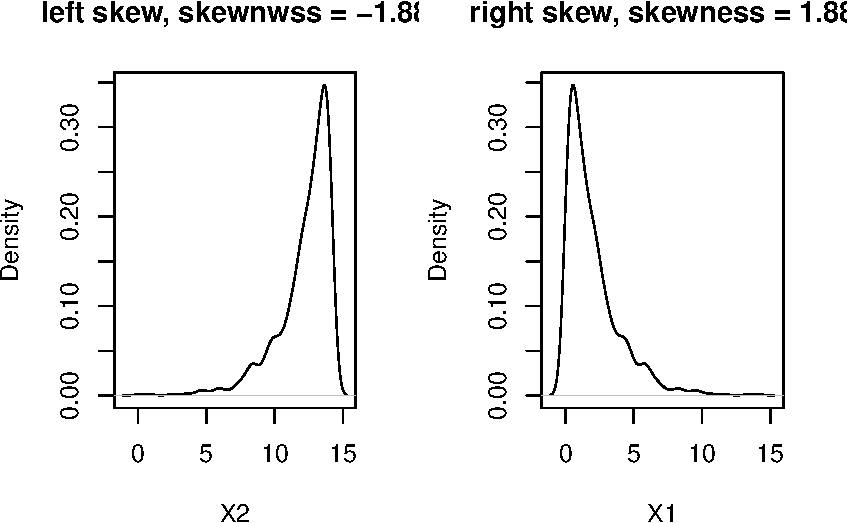
\includegraphics[width=0.8\linewidth]{CE_JSM2017_files/figure-latex/skew-1} 

}

\caption{Shewed Distribution}\label{fig:skew}
\end{figure}

You can easily tell if a distribution is skewed by simple
visualization(Figure@ref(fig:skew)). There are different ways may help
to remove skewness such as log, square root or inverse. However it is
often difficult to determine from plots which transformation is most
appropriate for correcting skewness. The Box-Cox procedure automatically
identified a transformation from the family of power transformations
that are indexed by a parameter \(\lambda\)(Box G
\protect\hyperlink{ref-BOXCOX1}{1964}).

\[
x^{*}=\begin{cases}
\begin{array}{c}
\frac{x^{\lambda}-1}{\lambda}\\
log(x)
\end{array} & \begin{array}{c}
if\ \lambda\neq0\\
if\ \lambda=0
\end{array}\end{cases}
\]

It is easy to see that this family includes log transformation
(\(\lambda=0\)), square transformation (\(\lambda=2\)), square root
(\(\lambda=0.5\)), inverse (\(\lambda=-1\)) and others in-between. We
can still use function \texttt{preProcess()} in package \texttt{caret}
to apply this transformation by chaning the \texttt{method} argument.

\begin{Shaded}
\begin{Highlighting}[]
\KeywordTok{describe}\NormalTok{(sim.dat)}
\end{Highlighting}
\end{Shaded}

\begin{verbatim}
##              vars    n      mean       sd   median   trimmed      mad      min
## age             1  999     38.58    14.19    36.00     37.67    16.31    16.00
## gender*         2 1000      1.45     0.50     1.00      1.43     0.00     1.00
## income          3  816 113543.07 49842.29 93868.68 104841.94 28989.47 41775.64
## house*          4 1000      1.57     0.50     2.00      1.58     0.00     1.00
## store_exp       5  999   1358.71  2775.17   329.80    845.14   197.47   155.81
## online_exp      6 1000   2120.18  1731.22  1941.86   1874.51  1015.21    68.82
## store_trans     7 1000      5.35     3.70     4.00      4.89     2.97     1.00
## online_trans    8 1000     13.55     7.96    14.00     13.42    10.38     1.00
## Q1              9 1000      3.10     1.45     3.00      3.13     1.48     1.00
## Q2             10 1000      1.82     1.17     1.00      1.65     0.00     1.00
## Q3             11 1000      1.99     1.40     1.00      1.75     0.00     1.00
## Q4             12 1000      2.76     1.16     3.00      2.83     1.48     1.00
## Q5             13 1000      2.94     1.28     4.00      3.05     0.00     1.00
## Q6             14 1000      2.45     1.44     2.00      2.43     1.48     1.00
## Q7             15 1000      3.43     1.46     4.00      3.54     0.00     1.00
## Q8             16 1000      2.40     1.15     2.00      2.36     1.48     1.00
## Q9             17 1000      3.08     1.12     4.00      3.23     0.00     1.00
## Q10            18 1000      2.32     1.14     2.00      2.27     1.48     1.00
## segment*       19 1000      2.70     1.15     3.00      2.75     1.48     1.00
##                    max     range  skew kurtosis      se
## age              69.00     53.00  0.47    -1.18    0.45
## gender*           2.00      1.00  0.22    -1.95    0.02
## income       319704.34 277928.70  1.69     2.57 1744.83
## house*            2.00      1.00 -0.27    -1.93    0.02
## store_exp     50000.00  49844.19  8.08   115.04   87.80
## online_exp     9479.44   9410.63  1.18     1.31   54.75
## store_trans      20.00     19.00  1.11     0.69    0.12
## online_trans     36.00     35.00  0.03    -0.98    0.25
## Q1                5.00      4.00 -0.12    -1.36    0.05
## Q2                5.00      4.00  1.13    -0.32    0.04
## Q3                5.00      4.00  1.06    -0.40    0.04
## Q4                5.00      4.00 -0.18    -1.46    0.04
## Q5                5.00      4.00 -0.60    -1.40    0.04
## Q6                5.00      4.00  0.11    -1.89    0.05
## Q7                5.00      4.00 -0.90    -0.79    0.05
## Q8                5.00      4.00  0.21    -1.33    0.04
## Q9                5.00      4.00 -0.68    -1.10    0.04
## Q10               5.00      4.00  0.39    -1.23    0.04
## segment*          4.00      3.00 -0.20    -1.41    0.04
\end{verbatim}

It is easy to see the skewed variables. If \texttt{mean} and
\texttt{trimmed} differ a lot, there is very likely outliers. By
default, \texttt{trimmed} reports mean by dropping the top and bottom
10\%. It can be adjusted by setting argument \texttt{trim=}. It is clear
that \texttt{store\_exp} has outliers.

As an example, we will apply Box-Cox transformation on
\texttt{store\_trans} and \texttt{online\_trans}:

\begin{Shaded}
\begin{Highlighting}[]
\CommentTok{# select the two columns and save them as dat_bc}
\NormalTok{dat_bc<-}\KeywordTok{subset}\NormalTok{(sim.dat,}\DataTypeTok{select=}\KeywordTok{c}\NormalTok{(}\StringTok{"store_trans"}\NormalTok{,}\StringTok{"online_trans"}\NormalTok{))}
\NormalTok{(trans<-}\KeywordTok{preProcess}\NormalTok{(dat_bc,}\DataTypeTok{method=}\KeywordTok{c}\NormalTok{(}\StringTok{"BoxCox"}\NormalTok{)))}
\end{Highlighting}
\end{Shaded}

\begin{verbatim}
## Created from 1000 samples and 2 variables
## 
## Pre-processing:
##   - Box-Cox transformation (2)
##   - ignored (0)
## 
## Lambda estimates for Box-Cox transformation:
## 0.1, 0.7
\end{verbatim}

The last line of the output shows the estimates of \(\lambda\) for each
variable. As before, use \texttt{predict()} to get the transformed
result:

\begin{Shaded}
\begin{Highlighting}[]
\NormalTok{transformed<-}\KeywordTok{predict}\NormalTok{(trans,dat_bc)}
\KeywordTok{par}\NormalTok{(}\DataTypeTok{mfrow=}\KeywordTok{c}\NormalTok{(}\DecValTok{1}\NormalTok{,}\DecValTok{2}\NormalTok{),}\DataTypeTok{oma=}\KeywordTok{c}\NormalTok{(}\DecValTok{2}\NormalTok{,}\DecValTok{2}\NormalTok{,}\DecValTok{2}\NormalTok{,}\DecValTok{2}\NormalTok{))}
\KeywordTok{hist}\NormalTok{(dat_bc}\OperatorTok{$}\NormalTok{store_trans,}\DataTypeTok{main=}\StringTok{"Before Transformation"}\NormalTok{,}\DataTypeTok{xlab=}\StringTok{"store_trans"}\NormalTok{)}
\KeywordTok{hist}\NormalTok{(transformed}\OperatorTok{$}\NormalTok{store_trans,}\DataTypeTok{main=}\StringTok{"After Transformation"}\NormalTok{,}\DataTypeTok{xlab=}\StringTok{"store_trans"}\NormalTok{)}
\end{Highlighting}
\end{Shaded}

\begin{figure}

{\centering 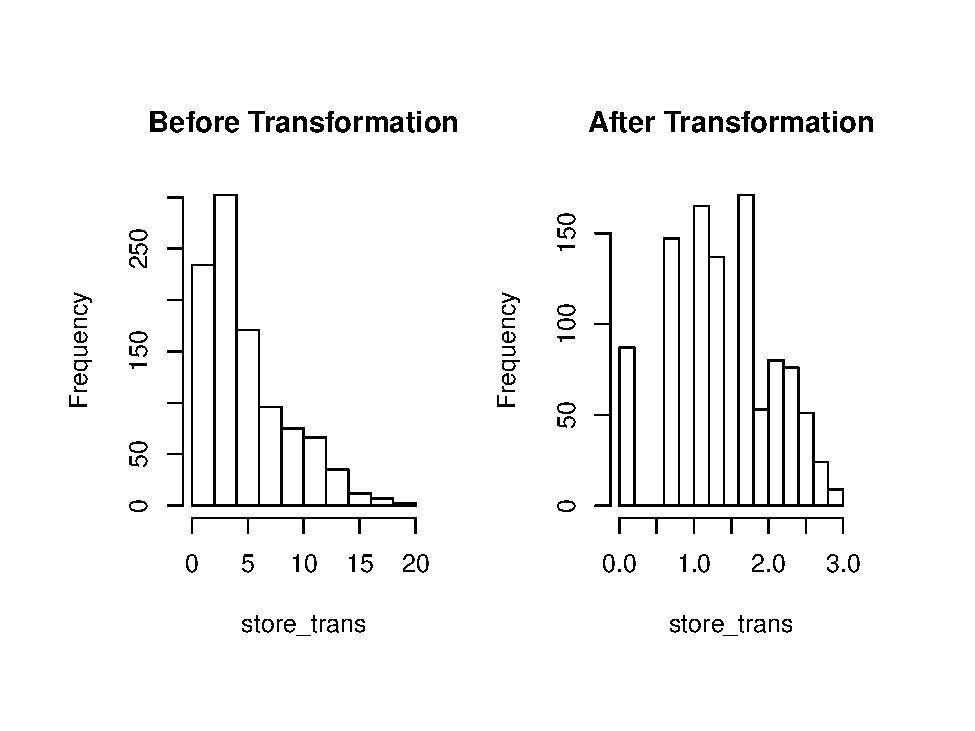
\includegraphics[width=0.8\linewidth]{CE_JSM2017_files/figure-latex/bc-1} 

}

\caption{Box-Cox Transformation}\label{fig:bc}
\end{figure}

Before the transformation, the \texttt{stroe\_trans} is skewed right.
The situation is significantly improved after (figure@ref(fig:bc)).
\texttt{BoxCoxTrans\ ()} can also conduct Box-Cox transform. But note
that \texttt{BoxCoxTrans\ ()} can only be applied to a single variable,
and it is not possible to transform difference columns in a data frame
at the same time.

\begin{Shaded}
\begin{Highlighting}[]
\NormalTok{(trans<-}\KeywordTok{BoxCoxTrans}\NormalTok{(dat_bc}\OperatorTok{$}\NormalTok{store_trans))}
\end{Highlighting}
\end{Shaded}

\begin{verbatim}
## Box-Cox Transformation
## 
## 1000 data points used to estimate Lambda
## 
## Input data summary:
##    Min. 1st Qu.  Median    Mean 3rd Qu.    Max. 
##    1.00    3.00    4.00    5.35    7.00   20.00 
## 
## Largest/Smallest: 20 
## Sample Skewness: 1.11 
## 
## Estimated Lambda: 0.1 
## With fudge factor, Lambda = 0 will be used for transformations
\end{verbatim}

\begin{Shaded}
\begin{Highlighting}[]
\NormalTok{transformed<-}\KeywordTok{predict}\NormalTok{(trans,dat_bc}\OperatorTok{$}\NormalTok{store_trans)}
\KeywordTok{skewness}\NormalTok{(transformed)}
\end{Highlighting}
\end{Shaded}

\begin{verbatim}
## [1] -0.2154708
\end{verbatim}

The estimate of \(\lambda\) is the same as before (0.1). The skewness of
the original observation is 1.1, and -0.2 after transformation. Although
it is not strictly 0, it is greatly improved.

\hypertarget{resolve-outliers}{%
\subsection{Resolve Outliers}\label{resolve-outliers}}

Even under certain assumptions we can statistically define outliers, it
can be hard to define in some situations. Box plot, histogram and some
other basic visualizations can be used to initially check whether there
are outliers. For example, we can visualize numerical non-survey
variables in \texttt{sim.dat}:

\begin{Shaded}
\begin{Highlighting}[]
\CommentTok{# select numerical non-survey data}
\NormalTok{sdat<-}\KeywordTok{subset}\NormalTok{(sim.dat,}\DataTypeTok{select=}\KeywordTok{c}\NormalTok{(}\StringTok{"age"}\NormalTok{,}\StringTok{"income"}\NormalTok{,}\StringTok{"store_exp"}\NormalTok{,}\StringTok{"online_exp"}\NormalTok{,}\StringTok{"store_trans"}\NormalTok{,}\StringTok{"online_trans"}\NormalTok{ ))}
\CommentTok{# use scatterplotMatrix() function from car package}
\KeywordTok{par}\NormalTok{(}\DataTypeTok{oma=}\KeywordTok{c}\NormalTok{(}\DecValTok{2}\NormalTok{,}\DecValTok{2}\NormalTok{,}\DecValTok{1}\NormalTok{,}\DecValTok{2}\NormalTok{))}
\KeywordTok{scatterplotMatrix}\NormalTok{(sdat,}\DataTypeTok{diagonal=}\StringTok{"boxplot"}\NormalTok{,}\DataTypeTok{smoother=}\OtherTok{FALSE}\NormalTok{)}
\end{Highlighting}
\end{Shaded}

\begin{verbatim}
## Warning in applyDefaults(diagonal, defaults = list(method =
## "adaptiveDensity"), : unnamed diag arguments, will be ignored
\end{verbatim}

\begin{verbatim}
## Warning in plot.window(...): "smoother" is not a graphical parameter
\end{verbatim}

\begin{verbatim}
## Warning in plot.xy(xy, type, ...): "smoother" is not a graphical parameter
\end{verbatim}

\begin{verbatim}
## Warning in title(...): "smoother" is not a graphical parameter
\end{verbatim}

\begin{verbatim}
## Warning in plot.window(...): "smoother" is not a graphical parameter
\end{verbatim}

\begin{verbatim}
## Warning in plot.xy(xy, type, ...): "smoother" is not a graphical parameter
\end{verbatim}

\begin{verbatim}
## Warning in title(...): "smoother" is not a graphical parameter
\end{verbatim}

\begin{verbatim}
## Warning in axis(side = side, at = at, labels = labels, ...): "smoother" is not a
## graphical parameter
\end{verbatim}

\begin{verbatim}
## Warning in plot.window(...): "smoother" is not a graphical parameter
\end{verbatim}

\begin{verbatim}
## Warning in plot.xy(xy, type, ...): "smoother" is not a graphical parameter
\end{verbatim}

\begin{verbatim}
## Warning in title(...): "smoother" is not a graphical parameter
\end{verbatim}

\begin{verbatim}
## Warning in plot.window(...): "smoother" is not a graphical parameter
\end{verbatim}

\begin{verbatim}
## Warning in plot.xy(xy, type, ...): "smoother" is not a graphical parameter
\end{verbatim}

\begin{verbatim}
## Warning in title(...): "smoother" is not a graphical parameter
\end{verbatim}

\begin{verbatim}
## Warning in axis(side = side, at = at, labels = labels, ...): "smoother" is not a
## graphical parameter
\end{verbatim}

\begin{verbatim}
## Warning in plot.window(...): "smoother" is not a graphical parameter
\end{verbatim}

\begin{verbatim}
## Warning in plot.xy(xy, type, ...): "smoother" is not a graphical parameter
\end{verbatim}

\begin{verbatim}
## Warning in title(...): "smoother" is not a graphical parameter
\end{verbatim}

\begin{verbatim}
## Warning in plot.window(...): "smoother" is not a graphical parameter
\end{verbatim}

\begin{verbatim}
## Warning in plot.xy(xy, type, ...): "smoother" is not a graphical parameter
\end{verbatim}

\begin{verbatim}
## Warning in title(...): "smoother" is not a graphical parameter
\end{verbatim}

\begin{verbatim}
## Warning in axis(side = side, at = at, labels = labels, ...): "smoother" is not a
## graphical parameter

## Warning in axis(side = side, at = at, labels = labels, ...): "smoother" is not a
## graphical parameter
\end{verbatim}

\begin{verbatim}
## Warning in plot.window(...): "smoother" is not a graphical parameter
\end{verbatim}

\begin{verbatim}
## Warning in plot.xy(xy, type, ...): "smoother" is not a graphical parameter
\end{verbatim}

\begin{verbatim}
## Warning in title(...): "smoother" is not a graphical parameter
\end{verbatim}

\begin{verbatim}
## Warning in axis(side = side, at = at, labels = labels, ...): "smoother" is not a
## graphical parameter
\end{verbatim}

\begin{verbatim}
## Warning in plot.window(...): "smoother" is not a graphical parameter
\end{verbatim}

\begin{verbatim}
## Warning in plot.xy(xy, type, ...): "smoother" is not a graphical parameter
\end{verbatim}

\begin{verbatim}
## Warning in title(...): "smoother" is not a graphical parameter
\end{verbatim}

\begin{verbatim}
## Warning in plot.window(...): "smoother" is not a graphical parameter
\end{verbatim}

\begin{verbatim}
## Warning in plot.xy(xy, type, ...): "smoother" is not a graphical parameter
\end{verbatim}

\begin{verbatim}
## Warning in title(...): "smoother" is not a graphical parameter
\end{verbatim}

\begin{verbatim}
## Warning in plot.window(...): "smoother" is not a graphical parameter
\end{verbatim}

\begin{verbatim}
## Warning in plot.xy(xy, type, ...): "smoother" is not a graphical parameter
\end{verbatim}

\begin{verbatim}
## Warning in title(...): "smoother" is not a graphical parameter
\end{verbatim}

\begin{verbatim}
## Warning in plot.window(...): "smoother" is not a graphical parameter
\end{verbatim}

\begin{verbatim}
## Warning in plot.xy(xy, type, ...): "smoother" is not a graphical parameter
\end{verbatim}

\begin{verbatim}
## Warning in title(...): "smoother" is not a graphical parameter
\end{verbatim}

\begin{verbatim}
## Warning in plot.window(...): "smoother" is not a graphical parameter
\end{verbatim}

\begin{verbatim}
## Warning in plot.xy(xy, type, ...): "smoother" is not a graphical parameter
\end{verbatim}

\begin{verbatim}
## Warning in title(...): "smoother" is not a graphical parameter
\end{verbatim}

\begin{verbatim}
## Warning in plot.window(...): "smoother" is not a graphical parameter
\end{verbatim}

\begin{verbatim}
## Warning in plot.xy(xy, type, ...): "smoother" is not a graphical parameter
\end{verbatim}

\begin{verbatim}
## Warning in title(...): "smoother" is not a graphical parameter
\end{verbatim}

\begin{verbatim}
## Warning in plot.window(...): "smoother" is not a graphical parameter
\end{verbatim}

\begin{verbatim}
## Warning in plot.xy(xy, type, ...): "smoother" is not a graphical parameter
\end{verbatim}

\begin{verbatim}
## Warning in title(...): "smoother" is not a graphical parameter
\end{verbatim}

\begin{verbatim}
## Warning in plot.window(...): "smoother" is not a graphical parameter
\end{verbatim}

\begin{verbatim}
## Warning in plot.xy(xy, type, ...): "smoother" is not a graphical parameter
\end{verbatim}

\begin{verbatim}
## Warning in title(...): "smoother" is not a graphical parameter
\end{verbatim}

\begin{verbatim}
## Warning in plot.window(...): "smoother" is not a graphical parameter
\end{verbatim}

\begin{verbatim}
## Warning in plot.xy(xy, type, ...): "smoother" is not a graphical parameter
\end{verbatim}

\begin{verbatim}
## Warning in title(...): "smoother" is not a graphical parameter
\end{verbatim}

\begin{verbatim}
## Warning in plot.window(...): "smoother" is not a graphical parameter
\end{verbatim}

\begin{verbatim}
## Warning in plot.xy(xy, type, ...): "smoother" is not a graphical parameter
\end{verbatim}

\begin{verbatim}
## Warning in title(...): "smoother" is not a graphical parameter
\end{verbatim}

\begin{verbatim}
## Warning in plot.window(...): "smoother" is not a graphical parameter
\end{verbatim}

\begin{verbatim}
## Warning in plot.xy(xy, type, ...): "smoother" is not a graphical parameter
\end{verbatim}

\begin{verbatim}
## Warning in title(...): "smoother" is not a graphical parameter
\end{verbatim}

\begin{verbatim}
## Warning in axis(side = side, at = at, labels = labels, ...): "smoother" is not a
## graphical parameter
\end{verbatim}

\begin{verbatim}
## Warning in plot.window(...): "smoother" is not a graphical parameter
\end{verbatim}

\begin{verbatim}
## Warning in plot.xy(xy, type, ...): "smoother" is not a graphical parameter
\end{verbatim}

\begin{verbatim}
## Warning in title(...): "smoother" is not a graphical parameter
\end{verbatim}

\begin{verbatim}
## Warning in axis(side = side, at = at, labels = labels, ...): "smoother" is not a
## graphical parameter
\end{verbatim}

\begin{verbatim}
## Warning in plot.window(...): "smoother" is not a graphical parameter
\end{verbatim}

\begin{verbatim}
## Warning in plot.xy(xy, type, ...): "smoother" is not a graphical parameter
\end{verbatim}

\begin{verbatim}
## Warning in title(...): "smoother" is not a graphical parameter
\end{verbatim}

\begin{verbatim}
## Warning in plot.window(...): "smoother" is not a graphical parameter
\end{verbatim}

\begin{verbatim}
## Warning in plot.xy(xy, type, ...): "smoother" is not a graphical parameter
\end{verbatim}

\begin{verbatim}
## Warning in title(...): "smoother" is not a graphical parameter
\end{verbatim}

\begin{verbatim}
## Warning in plot.window(...): "smoother" is not a graphical parameter
\end{verbatim}

\begin{verbatim}
## Warning in plot.xy(xy, type, ...): "smoother" is not a graphical parameter
\end{verbatim}

\begin{verbatim}
## Warning in title(...): "smoother" is not a graphical parameter
\end{verbatim}

\begin{verbatim}
## Warning in plot.window(...): "smoother" is not a graphical parameter
\end{verbatim}

\begin{verbatim}
## Warning in plot.xy(xy, type, ...): "smoother" is not a graphical parameter
\end{verbatim}

\begin{verbatim}
## Warning in title(...): "smoother" is not a graphical parameter
\end{verbatim}

\begin{verbatim}
## Warning in plot.window(...): "smoother" is not a graphical parameter
\end{verbatim}

\begin{verbatim}
## Warning in plot.xy(xy, type, ...): "smoother" is not a graphical parameter
\end{verbatim}

\begin{verbatim}
## Warning in title(...): "smoother" is not a graphical parameter
\end{verbatim}

\begin{verbatim}
## Warning in plot.window(...): "smoother" is not a graphical parameter
\end{verbatim}

\begin{verbatim}
## Warning in plot.xy(xy, type, ...): "smoother" is not a graphical parameter
\end{verbatim}

\begin{verbatim}
## Warning in title(...): "smoother" is not a graphical parameter
\end{verbatim}

\begin{verbatim}
## Warning in plot.window(...): "smoother" is not a graphical parameter
\end{verbatim}

\begin{verbatim}
## Warning in plot.xy(xy, type, ...): "smoother" is not a graphical parameter
\end{verbatim}

\begin{verbatim}
## Warning in title(...): "smoother" is not a graphical parameter
\end{verbatim}

\begin{verbatim}
## Warning in plot.window(...): "smoother" is not a graphical parameter
\end{verbatim}

\begin{verbatim}
## Warning in plot.xy(xy, type, ...): "smoother" is not a graphical parameter
\end{verbatim}

\begin{verbatim}
## Warning in title(...): "smoother" is not a graphical parameter
\end{verbatim}

\begin{verbatim}
## Warning in plot.window(...): "smoother" is not a graphical parameter
\end{verbatim}

\begin{verbatim}
## Warning in plot.xy(xy, type, ...): "smoother" is not a graphical parameter
\end{verbatim}

\begin{verbatim}
## Warning in title(...): "smoother" is not a graphical parameter
\end{verbatim}

\begin{verbatim}
## Warning in plot.window(...): "smoother" is not a graphical parameter
\end{verbatim}

\begin{verbatim}
## Warning in plot.xy(xy, type, ...): "smoother" is not a graphical parameter
\end{verbatim}

\begin{verbatim}
## Warning in title(...): "smoother" is not a graphical parameter
\end{verbatim}

\begin{verbatim}
## Warning in plot.window(...): "smoother" is not a graphical parameter
\end{verbatim}

\begin{verbatim}
## Warning in plot.xy(xy, type, ...): "smoother" is not a graphical parameter
\end{verbatim}

\begin{verbatim}
## Warning in title(...): "smoother" is not a graphical parameter
\end{verbatim}

\begin{verbatim}
## Warning in axis(side = side, at = at, labels = labels, ...): "smoother" is not a
## graphical parameter
\end{verbatim}

\begin{verbatim}
## Warning in plot.window(...): "smoother" is not a graphical parameter
\end{verbatim}

\begin{verbatim}
## Warning in plot.xy(xy, type, ...): "smoother" is not a graphical parameter
\end{verbatim}

\begin{verbatim}
## Warning in title(...): "smoother" is not a graphical parameter
\end{verbatim}

\begin{verbatim}
## Warning in axis(side = side, at = at, labels = labels, ...): "smoother" is not a
## graphical parameter

## Warning in axis(side = side, at = at, labels = labels, ...): "smoother" is not a
## graphical parameter
\end{verbatim}

\begin{verbatim}
## Warning in plot.window(...): "smoother" is not a graphical parameter
\end{verbatim}

\begin{verbatim}
## Warning in plot.xy(xy, type, ...): "smoother" is not a graphical parameter
\end{verbatim}

\begin{verbatim}
## Warning in title(...): "smoother" is not a graphical parameter
\end{verbatim}

\begin{verbatim}
## Warning in plot.window(...): "smoother" is not a graphical parameter
\end{verbatim}

\begin{verbatim}
## Warning in plot.xy(xy, type, ...): "smoother" is not a graphical parameter
\end{verbatim}

\begin{verbatim}
## Warning in title(...): "smoother" is not a graphical parameter
\end{verbatim}

\begin{verbatim}
## Warning in axis(side = side, at = at, labels = labels, ...): "smoother" is not a
## graphical parameter
\end{verbatim}

\begin{verbatim}
## Warning in plot.window(...): "smoother" is not a graphical parameter
\end{verbatim}

\begin{verbatim}
## Warning in plot.xy(xy, type, ...): "smoother" is not a graphical parameter
\end{verbatim}

\begin{verbatim}
## Warning in title(...): "smoother" is not a graphical parameter
\end{verbatim}

\begin{verbatim}
## Warning in plot.window(...): "smoother" is not a graphical parameter
\end{verbatim}

\begin{verbatim}
## Warning in plot.xy(xy, type, ...): "smoother" is not a graphical parameter
\end{verbatim}

\begin{verbatim}
## Warning in title(...): "smoother" is not a graphical parameter
\end{verbatim}

\begin{verbatim}
## Warning in axis(side = side, at = at, labels = labels, ...): "smoother" is not a
## graphical parameter
\end{verbatim}

\begin{verbatim}
## Warning in plot.window(...): "smoother" is not a graphical parameter
\end{verbatim}

\begin{verbatim}
## Warning in plot.xy(xy, type, ...): "smoother" is not a graphical parameter
\end{verbatim}

\begin{verbatim}
## Warning in title(...): "smoother" is not a graphical parameter
\end{verbatim}

\begin{center}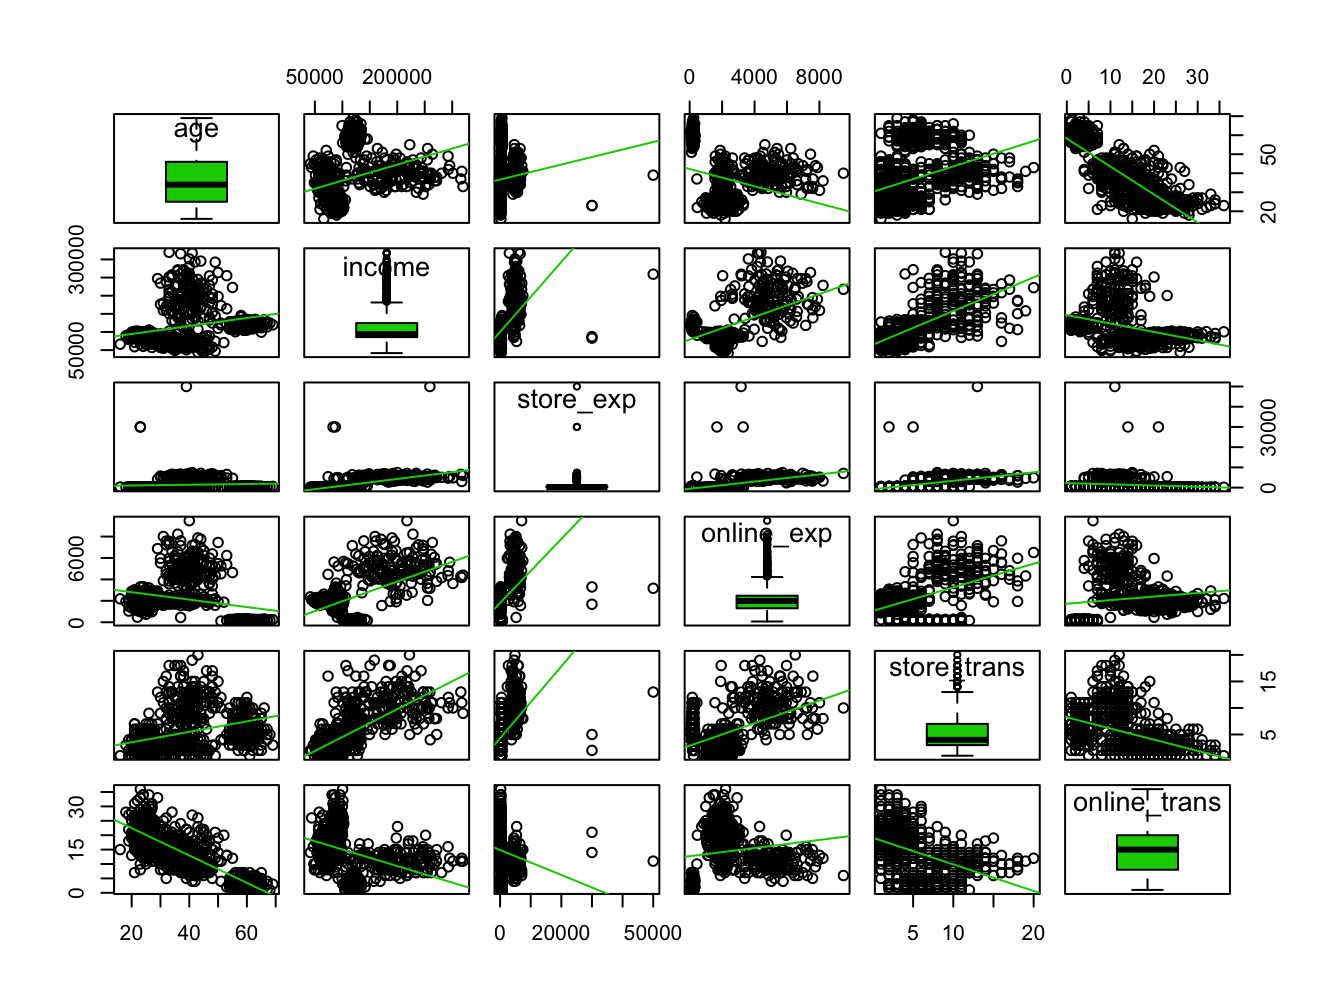
\includegraphics[width=0.8\linewidth]{CE_JSM2017_files/figure-latex/scm-1} \end{center}

As figure @ref(fig:scm) shows, \texttt{store\_exp} has outliers. It is
also easy to observe the pair relationship from the plot. \texttt{age}
is negatively correlated with \texttt{online\_trans} but positively
correlated with \texttt{store\_trans}. It seems that older people tend
to purchase from the local store. The amount of expense is positively
correlated with income. Scatterplot matrix like this can reveal lots of
information before modeling.

In addition to visualization, there are some statistical methods to
define outliers, such as the commonly used Z-score. The Z-score for
variable \(\mathbf{Y}\) is defined as:

\[Z_{i}=\frac{Y_{i}-\bar{Y}}{s}\]

where \(\bar{Y}\) and \(s\) are mean and standard deviation for \(Y\).
Z-score is a measurement of the distance between each observation and
the mean. This method may be misleading, especially when the sample size
is small. Iglewicz and Hoaglin proposed to use the modified Z-score to
determine the outlier(Iglewicz and Hoaglin
\protect\hyperlink{ref-mad1}{1993}):

\[M_{i}=\frac{0.6745(Y_{i}-\bar{Y})}{MAD}\]

Where MAD is the median of a series of \$\textbar{} Y\_ \{i\} -
\bar\{Y\} \textbar{} \$, called the median of the absolute dispersion.
Iglewicz and Hoaglin suggest that the points with the Z-score greater
than 3.5 corrected above are possible outliers. Let's apply it to
\texttt{income}:

\begin{Shaded}
\begin{Highlighting}[]
\CommentTok{# calculate median of the absolute dispersion for income}
\NormalTok{ymad<-}\KeywordTok{mad}\NormalTok{(}\KeywordTok{na.omit}\NormalTok{(sdat}\OperatorTok{$}\NormalTok{income))}
\CommentTok{# calculate z-score}
\NormalTok{zs<-(sdat}\OperatorTok{$}\NormalTok{income}\OperatorTok{-}\KeywordTok{mean}\NormalTok{(}\KeywordTok{na.omit}\NormalTok{(sdat}\OperatorTok{$}\NormalTok{income)))}\OperatorTok{/}\NormalTok{ymad}
\CommentTok{# count the number of outliers}
\KeywordTok{sum}\NormalTok{(}\KeywordTok{na.omit}\NormalTok{(zs}\OperatorTok{>}\FloatTok{3.5}\NormalTok{))}
\end{Highlighting}
\end{Shaded}

\begin{verbatim}
## [1] 59
\end{verbatim}

According to modified Z-score, variable income has 59 outliers. Refer to
(Iglewicz and Hoaglin \protect\hyperlink{ref-mad1}{1993}) for other ways
of detecting outliers.

The impact of outliers depends on the model. Some models are sensitive
to outliers, such as linear regression, logistic regression. Some are
pretty robust to outliers, such as tree models, support vector machine.
Also, the outlier is not wrong data. It is real observation so can not
be deleted at will. If a model is sensitive to outliers, we can use
\emph{spatial sign transformation} (Serneels S
\protect\hyperlink{ref-ssp}{2006}) to minimize the problem. It projects
the original sample points to the surface of a sphere by:

\[x_{ij}^{*}=\frac{x_{ij}}{\sqrt{\sum_{j=1}^{p}x_{ij}^{2}}}\]

where \(x_{ij}\) represents the \(i^{th}\) observation and \(j^{th}\)
variable. As shown in the equation, every observation for sample \(i\)
is divided by its square mode. The denominator is the Euclidean distance
to the center of the p-dimensional predictor space. Three things to pay
attention here:

\begin{enumerate}
\def\labelenumi{\arabic{enumi}.}
\tightlist
\item
  It is important to center and scale the predictor data before using
  this transformation
\item
  Unlike centering or scaling, this manipulation of the predictors
  transforms them as a group
\item
  If there are some variables to remove (for example, highly correlated
  variables), do it before the transformation
\end{enumerate}

Function \texttt{spatialSign()} \texttt{caret} package can conduct the
transformation. Take \texttt{income} and \texttt{age} as an example:

\begin{Shaded}
\begin{Highlighting}[]
\CommentTok{# KNN imputation}
\NormalTok{sdat<-sim.dat[,}\KeywordTok{c}\NormalTok{(}\StringTok{"income"}\NormalTok{,}\StringTok{"age"}\NormalTok{)]}
\NormalTok{imp<-}\KeywordTok{preProcess}\NormalTok{(sdat,}\DataTypeTok{method=}\KeywordTok{c}\NormalTok{(}\StringTok{"knnImpute"}\NormalTok{),}\DataTypeTok{k=}\DecValTok{5}\NormalTok{)}
\NormalTok{sdat<-}\KeywordTok{predict}\NormalTok{(imp,sdat)}
\NormalTok{transformed <-}\StringTok{ }\KeywordTok{spatialSign}\NormalTok{(sdat)}
\NormalTok{transformed <-}\StringTok{ }\KeywordTok{as.data.frame}\NormalTok{(transformed)}
\KeywordTok{par}\NormalTok{(}\DataTypeTok{mfrow=}\KeywordTok{c}\NormalTok{(}\DecValTok{1}\NormalTok{,}\DecValTok{2}\NormalTok{),}\DataTypeTok{oma=}\KeywordTok{c}\NormalTok{(}\DecValTok{2}\NormalTok{,}\DecValTok{2}\NormalTok{,}\DecValTok{2}\NormalTok{,}\DecValTok{2}\NormalTok{))}
\KeywordTok{plot}\NormalTok{(income }\OperatorTok{~}\StringTok{ }\NormalTok{age,}\DataTypeTok{data =}\NormalTok{ sdat,}\DataTypeTok{col=}\StringTok{"blue"}\NormalTok{,}\DataTypeTok{main=}\StringTok{"Before"}\NormalTok{)}
\KeywordTok{plot}\NormalTok{(income }\OperatorTok{~}\StringTok{ }\NormalTok{age,}\DataTypeTok{data =}\NormalTok{ transformed,}\DataTypeTok{col=}\StringTok{"blue"}\NormalTok{,}\DataTypeTok{main=}\StringTok{"After"}\NormalTok{)}
\end{Highlighting}
\end{Shaded}

\begin{figure}

{\centering 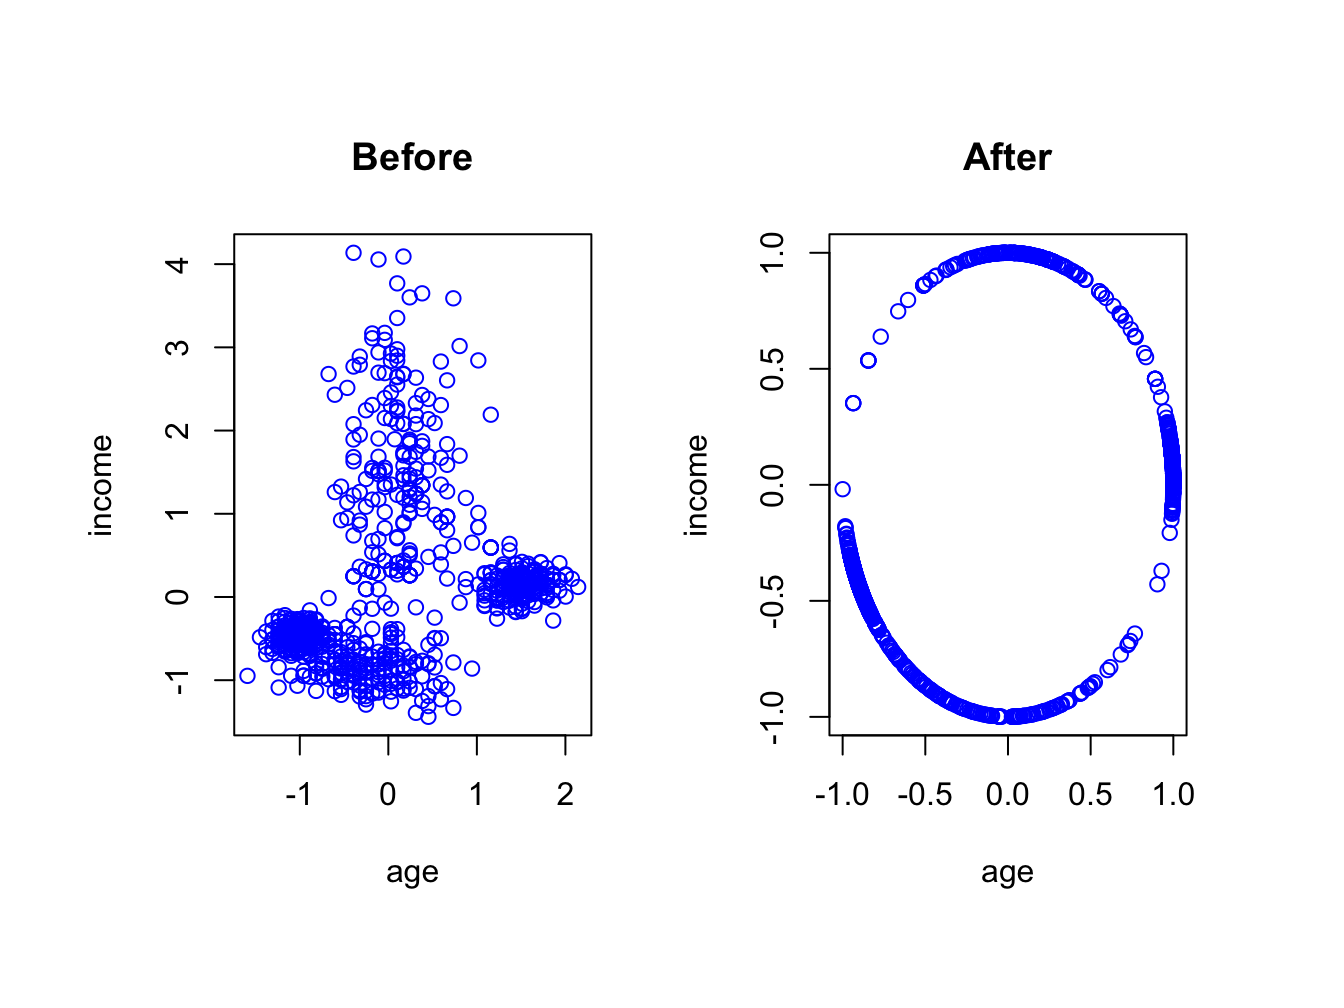
\includegraphics[width=0.8\linewidth]{CE_JSM2017_files/figure-latex/sst-1} 

}

\caption{spatial sign transformation}\label{fig:sst}
\end{figure}

Some readers may have found that the above code does not seem to
standardize the data before transformation. Recall the introduction of
KNN, \texttt{preProcess\ ()} with \texttt{method="knnImpute"} by default
will standardize data.

\hypertarget{collinearity}{%
\subsection{Collinearity}\label{collinearity}}

It is probably a technical term that many un-technical people also know.
There is an excellent function in \texttt{corrplot} package with the
same name \texttt{corrplot()} that can visualize correlation structure
of a set of predictors. The function has the option to reorder the
variables in a way that reveals clusters of highly correlated ones.

\begin{Shaded}
\begin{Highlighting}[]
\CommentTok{# select non-survey numerical variables}
\NormalTok{sdat<-}\KeywordTok{subset}\NormalTok{(sim.dat,}\DataTypeTok{select=}\KeywordTok{c}\NormalTok{(}\StringTok{"age"}\NormalTok{,}\StringTok{"income"}\NormalTok{,}\StringTok{"store_exp"}\NormalTok{,}\StringTok{"online_exp"}\NormalTok{,}\StringTok{"store_trans"}\NormalTok{,}\StringTok{"online_trans"}\NormalTok{ ))}
\CommentTok{# use bagging imputation here}
\NormalTok{imp<-}\KeywordTok{preProcess}\NormalTok{(sdat,}\DataTypeTok{method=}\StringTok{"bagImpute"}\NormalTok{)}
\NormalTok{sdat<-}\KeywordTok{predict}\NormalTok{(imp,sdat)}
\CommentTok{# get the correlation matrix}
\NormalTok{correlation<-}\KeywordTok{cor}\NormalTok{(sdat)}
\CommentTok{# plot }
\KeywordTok{par}\NormalTok{(}\DataTypeTok{oma=}\KeywordTok{c}\NormalTok{(}\DecValTok{2}\NormalTok{,}\DecValTok{2}\NormalTok{,}\DecValTok{2}\NormalTok{,}\DecValTok{2}\NormalTok{))}
\KeywordTok{corrplot.mixed}\NormalTok{(correlation,}\DataTypeTok{order=}\StringTok{"hclust"}\NormalTok{,}\DataTypeTok{tl.pos=}\StringTok{"lt"}\NormalTok{,}\DataTypeTok{upper=}\StringTok{"ellipse"}\NormalTok{)}
\end{Highlighting}
\end{Shaded}

\begin{center}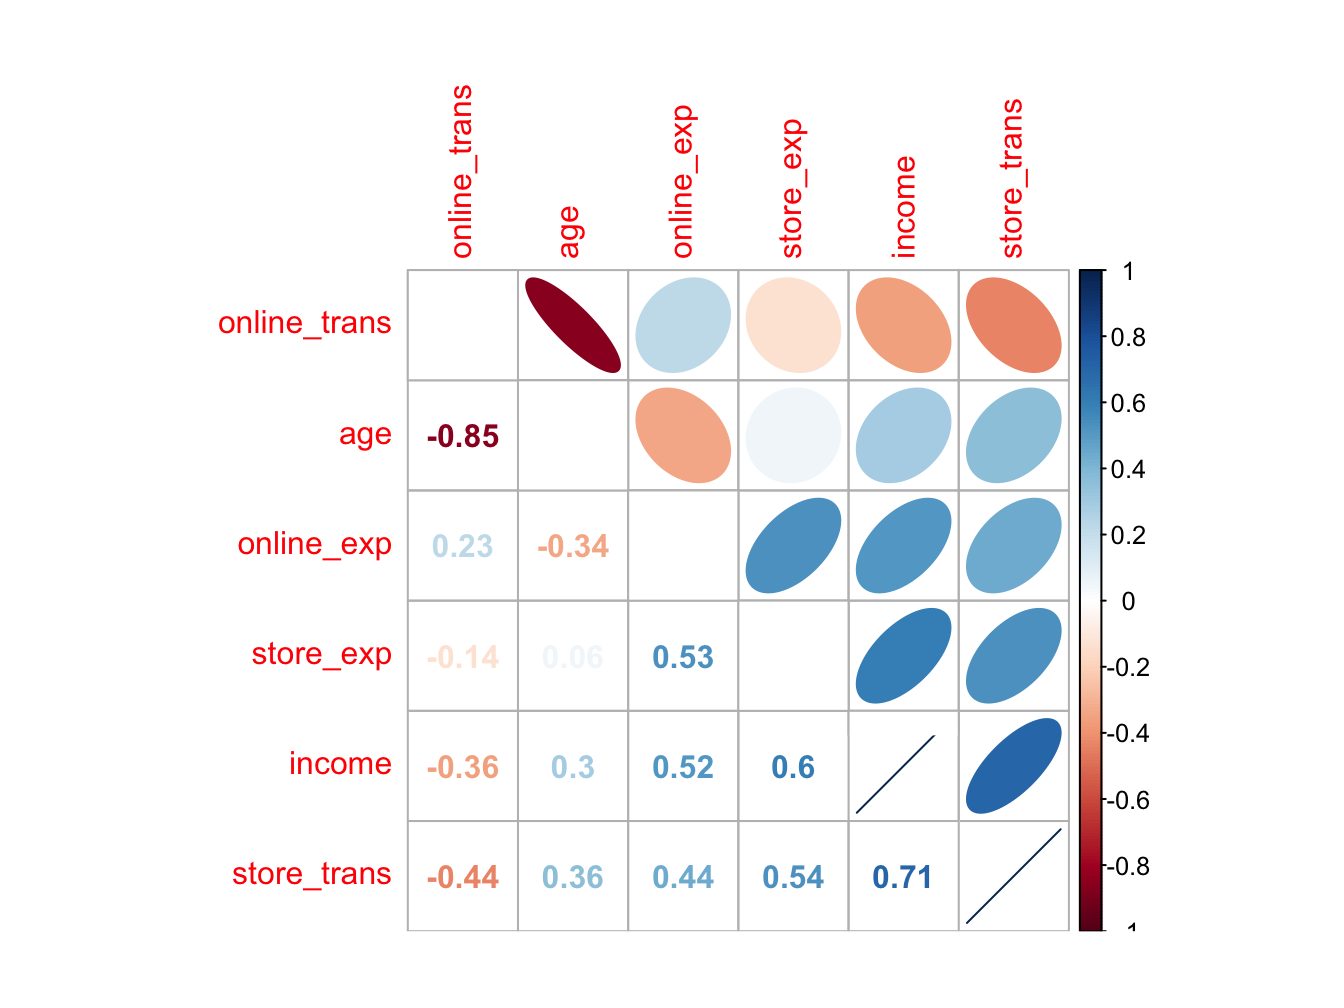
\includegraphics[width=0.8\linewidth]{CE_JSM2017_files/figure-latex/corp-1} \end{center}

Here use \texttt{corrplot.mixed()} function to visualize the correlation
matrix (figure @ref(fig:corp)). The closer the correlation is to 0, the
lighter the color is and the closer the shape is to a circle. The
elliptical means the correlation is not equal to 0 (because we set the
\texttt{upper\ =\ "ellipse"}), the greater the correlation, the narrower
the ellipse. Blue represents a positive correlation, red represents a
negative correlation. The direction of the ellipse also changes with the
correlation. The correlation coefficient is shown in the lower triangle
of the matrix. The variables relationship from previous scatter matrix
(figure @ref(fig: scm)) are clear here: the negative correlation between
age and online shopping, the positive correlation between income and
amount of purchasing. Some correlation is very strong ( such as the
correlation between \texttt{online\_trans} and\texttt{age} is -0.85)
which means the two variables contain duplicate information

. Section 3.5 of ``Applied Predictive Modeling'' (Max Kuhn
\protect\hyperlink{ref-APM}{2013}) presents a heuristic algorithm to
remove a minimum number of predictors to ensure all pairwise
correlations are below a certain threshold:

\begin{quote}
\begin{enumerate}
\def\labelenumi{(\arabic{enumi})}
\tightlist
\item
  Calculate the correlation matrix of the predictors.
\item
  Determine the two predictors associated with the largest absolute
  pairwise correlation (call them predictors A and B).
\item
  Determine the average correlation between A and the other variables.
  Do the same for predictor B.
\item
  If A has a larger average correlation, remove it; otherwise, remove
  predictor B.
\item
  Repeat Step 2-4 until no absolute correlations are above the
  threshold.
\end{enumerate}
\end{quote}

The \texttt{findCorrelation()} function in package \texttt{caret} will
apply the above algorithm.

\begin{Shaded}
\begin{Highlighting}[]
\NormalTok{(highCorr<-}\KeywordTok{findCorrelation}\NormalTok{(}\KeywordTok{cor}\NormalTok{(sdat),}\DataTypeTok{cutoff=}\NormalTok{.}\DecValTok{75}\NormalTok{))}
\end{Highlighting}
\end{Shaded}

\begin{verbatim}
## [1] 1
\end{verbatim}

It returns the index of columns need to be deleted. It tells us that we
need to remove the first column to make sure the correlations are all
below 0.75.

\begin{Shaded}
\begin{Highlighting}[]
\CommentTok{# delete highly correlated columns}
\NormalTok{sdat<-sdat[}\OperatorTok{-}\NormalTok{highCorr]}
\CommentTok{# check the new correlation matrix}
\KeywordTok{cor}\NormalTok{(sdat)}
\end{Highlighting}
\end{Shaded}

\begin{verbatim}
##                  income  store_exp online_exp store_trans online_trans
## income        1.0000000  0.6004006  0.5198623   0.7069595   -0.3572884
## store_exp     0.6004006  1.0000000  0.5349527   0.5399121   -0.1367411
## online_exp    0.5198623  0.5349527  1.0000000   0.4420638    0.2256370
## store_trans   0.7069595  0.5399121  0.4420638   1.0000000   -0.4367544
## online_trans -0.3572884 -0.1367411  0.2256370  -0.4367544    1.0000000
\end{verbatim}

The absolute value of the elements in the correlation matrix after
removal are all below 0.75.

\hypertarget{sparse-variables}{%
\subsection{Sparse Variables}\label{sparse-variables}}

Other than the highly related predictors, predictors with degenerate
distributions can cause the problem too. Removing those variables can
significantly improve some models' performance and stability (such as
linear regression and logistic regression but the tree based model is
impervious to this type of predictors). One extreme example is a
variable with a single value which is called zero-variance variable.
Variables with very low frequency of unique values are near-zero
variance predictors. In general, detecting those variables follows two
rules:

\begin{itemize}
\tightlist
\item
  The fraction of unique values over the sample size
\item
  The ratio of the frequency of the most prevalent value to the
  frequency of the second most prevalent value.
\end{itemize}

\texttt{nearZeroVar()} function in the \texttt{caret} package can filter
near-zero variance predictors according to the above rules. In order to
show the useage of the function, let's arbitaryly add some problematic
variables to the origional data \texttt{sim.dat}:

\begin{Shaded}
\begin{Highlighting}[]
\CommentTok{# make a copy}
\NormalTok{zero_demo<-sim.dat}
\CommentTok{# add two sparse variable}
\CommentTok{# zero1 only has one unique value}
\CommentTok{# zero2 is a vector with the first element 1 and the rest are 0s}
\NormalTok{zero_demo}\OperatorTok{$}\NormalTok{zero1<-}\KeywordTok{rep}\NormalTok{(}\DecValTok{1}\NormalTok{,}\KeywordTok{nrow}\NormalTok{(zero_demo))}
\NormalTok{zero_demo}\OperatorTok{$}\NormalTok{zero2<-}\KeywordTok{c}\NormalTok{(}\DecValTok{1}\NormalTok{,}\KeywordTok{rep}\NormalTok{(}\DecValTok{0}\NormalTok{,}\KeywordTok{nrow}\NormalTok{(zero_demo)}\OperatorTok{-}\DecValTok{1}\NormalTok{))}
\end{Highlighting}
\end{Shaded}

The function will return a vector of integers indicating which columns
to remove:

\begin{Shaded}
\begin{Highlighting}[]
\KeywordTok{nearZeroVar}\NormalTok{(zero_demo,}\DataTypeTok{freqCut =} \DecValTok{95}\OperatorTok{/}\DecValTok{5}\NormalTok{, }\DataTypeTok{uniqueCut =} \DecValTok{10}\NormalTok{)}
\end{Highlighting}
\end{Shaded}

As expected, it returns the two columns we generated. You can go ahead
to remove them. Note the two arguments in the function
\texttt{freqCut\ =} and \texttt{uniqueCut\ =} are corresponding to the
previous two rules.

\begin{itemize}
\tightlist
\item
  \texttt{freqCut}: the cutoff for the ratio of the most common value to
  the second most common value
\item
  \texttt{uniqueCut}: the cutoff for the percentage of distinct values
  out of the number of total samples
\end{itemize}

\hypertarget{re-encode-dummy-variables}{%
\subsection{Re-encode Dummy Variables}\label{re-encode-dummy-variables}}

A dummy variable is a binary variable (0/1) to represent subgroups of
the sample. Sometimes we need to recode categories to smaller bits of
information named ``dummy variables''. For example, some questionnaires
have five options for each question, A, B, C, D, and E. After you get
the data, you will usually convert the corresponding categorical
variables for each question into five nominal variables, and then use
one of the options as the baseline.

Let's encode \texttt{gender} and \texttt{house} from \texttt{sim.dat} to
dummy variables. There are two ways to implement this. The first is to
use \texttt{class.ind()} from \texttt{nnet} package. However, it only
works on one variable at a time.

\begin{Shaded}
\begin{Highlighting}[]
\NormalTok{dumVar<-}\KeywordTok{class.ind}\NormalTok{(sim.dat}\OperatorTok{$}\NormalTok{gender)}
\KeywordTok{head}\NormalTok{(dumVar)}
\end{Highlighting}
\end{Shaded}

\begin{verbatim}
##      Female Male
## [1,]      1    0
## [2,]      1    0
## [3,]      0    1
## [4,]      0    1
## [5,]      0    1
## [6,]      0    1
\end{verbatim}

Since it is redundant to keep both, we need to remove one of them when
modeling. Another more powerful function is \texttt{dummyVars()} from
\texttt{caret}:

\begin{Shaded}
\begin{Highlighting}[]
\NormalTok{dumMod<-}\KeywordTok{dummyVars}\NormalTok{(}\OperatorTok{~}\NormalTok{gender}\OperatorTok{+}\NormalTok{house}\OperatorTok{+}\NormalTok{income,}
                  \DataTypeTok{data=}\NormalTok{sim.dat,}
                  \CommentTok{# use "origional variable name + level" as new name}
                  \DataTypeTok{levelsOnly=}\NormalTok{F)}
\KeywordTok{head}\NormalTok{(}\KeywordTok{predict}\NormalTok{(dumMod,sim.dat))}
\end{Highlighting}
\end{Shaded}

\begin{verbatim}
##   gender.Female gender.Male house.No house.Yes   income
## 1             1           0        0         1 120963.4
## 2             1           0        0         1 122008.1
## 3             0           1        0         1 114202.3
## 4             0           1        0         1 113616.3
## 5             0           1        0         1 124252.6
## 6             0           1        0         1 107661.5
\end{verbatim}

\texttt{dummyVars()} can also use formula format. The variable on the
right-hand side can be both categorical and numeric. For numerical
variable, the function will keep the variable unchanged. The advantage
is that you can apply the function to a data frame without removing
numerical variables. Other than that, the function can create
interaction term:

\begin{Shaded}
\begin{Highlighting}[]
\NormalTok{dumMod<-}\KeywordTok{dummyVars}\NormalTok{(}\OperatorTok{~}\NormalTok{gender}\OperatorTok{+}\NormalTok{house}\OperatorTok{+}\NormalTok{income}\OperatorTok{+}\NormalTok{income}\OperatorTok{:}\NormalTok{gender,}
                  \DataTypeTok{data=}\NormalTok{sim.dat,}
                  \DataTypeTok{levelsOnly=}\NormalTok{F)}
\KeywordTok{head}\NormalTok{(}\KeywordTok{predict}\NormalTok{(dumMod,sim.dat))}
\end{Highlighting}
\end{Shaded}

\begin{verbatim}
##   gender.Female gender.Male house.No house.Yes   income genderFemale:income
## 1             1           0        0         1 120963.4            120963.4
## 2             1           0        0         1 122008.1            122008.1
## 3             0           1        0         1 114202.3                 0.0
## 4             0           1        0         1 113616.3                 0.0
## 5             0           1        0         1 124252.6                 0.0
## 6             0           1        0         1 107661.5                 0.0
##   genderMale:income
## 1               0.0
## 2               0.0
## 3          114202.3
## 4          113616.3
## 5          124252.6
## 6          107661.5
\end{verbatim}

If you think the impact income levels on purchasing behavior is
different for male and female, then you may add the interaction term
between \texttt{income} and \texttt{gender}. You can do this by adding
\texttt{income:\ gender} in the formula.

\hypertarget{dynamicreproducible-report}{%
\section{Dynamic/Reproducible Report}\label{dynamicreproducible-report}}

\hypertarget{what-is-r-markdown}{%
\subsection{What is R Markdown?}\label{what-is-r-markdown}}

Let's start from markdown. Markdown is a lightweight markup language
designed to make authoring content easy for everyone. Here is a
definition of markup language:

\begin{quote}
Markup languages are designed for the processing, definition, and
presentation of text. The language specifies code for formatting, both
the layout and style, within a text file. The code used to specify the
format are called tags.
\end{quote}

HTML is an example of a widely known and used markup language.

Rather than writing complex markup code (e.g.~LyX, XML, HTML or LaTeX),
Markdown enables the use of a syntax much more like plain-text email. It
is young compared to the other markup languages. What makes markdown
distinct is that it is both machine-readable and human-readable.

R Markdown combines the core syntax of Markdown and embedded R code
chunks that are run so their output can be included in the final
document. Consider how people typically create an analytical report. The
author makes the graph/table, saves it as a file, and then copy and
pastes it into the final report. This process relies on manual labor.
The author may take a deep breath when the report is finally
well-shaped. If the data changes, the author must repeat the entire
process to update the graph.

\includegraphics{http://linhui.org/images/Jokes/DoProgrammingRight.png}

R Markdown comes to rescue! It provides an authoring framework for data
science. You can use a single R Markdown file to do both:

\begin{itemize}
\tightlist
\item
  save and execute code
\item
  generate high-quality reports that can be shared with an audience
\end{itemize}

R Markdown documents are fully reproducible and the most important and
it is simple!

\hypertarget{how-to-start}{%
\subsection{How to Start?}\label{how-to-start}}

\hypertarget{how-it-works}{%
\subsubsection{How It Works?}\label{how-it-works}}

When you run \texttt{render}, R Markdown feeds the \texttt{.rmd} file to
\texttt{knitr}.\texttt{knitr} is an R package that will execute all of
the code chunks and creates a new markdown (.md) document which includes
the code and its output. The markdown file is then processed by
\texttt{pandoc} which is responsible for creating the finished format.
\texttt{pandoc} is a swiss-knife to convert files from one markup format
into another.

\includegraphics{http://scientistcafe.com/CE_JSM2017/images/RMarkdownFlow.png}

R Markdown encapsulates all of the above processing into a single render
function.

\hypertarget{get-started}{%
\subsubsection{Get Started}\label{get-started}}

Install R and RStudio. If you have RStudio installed ready, I suggest
you make sure it is in the latest version. You can install the
\texttt{rmarkdown} package from CRAN with:

\begin{Shaded}
\begin{Highlighting}[]
\KeywordTok{install.packages}\NormalTok{(}\StringTok{"rmarkdown"}\NormalTok{)}
\end{Highlighting}
\end{Shaded}

R Markdown file is a plain text file that has the extension
\texttt{.Rmd}. You can create a sample \texttt{.Rmd} file in R Studio:

\includegraphics{http://scientistcafe.com/CE_JSM2017/images/newmd1.PNG}

Input your document title and author name and click ``OK'':

\includegraphics{http://scientistcafe.com/CE_JSM2017/images/newmd2.PNG}

The file contains three types of content:

\begin{itemize}
\tightlist
\item
  An (optional) YAML header surrounded by \texttt{-\/-\/-}
\item
  R code chunks surrounded by
  \texttt{\textasciigrave{}\textasciigrave{}\textasciigrave{}\{r\}} and
  \texttt{\textasciigrave{}\textasciigrave{}\textasciigrave{}}
\item
  text mixed with simple text formatting
\end{itemize}

R Markdown generates a new file that contains selected text, code, and
results from the \texttt{.Rmd} file. The new file can be in the
following formats:

\begin{itemize}
\tightlist
\item
  HTML
\item
  PDF
\item
  MS Word document
\item
  slide show
\item
  book
\item
  dashboard
\item
  package vignette
\item
  Others
\end{itemize}

\hypertarget{markdown-basic}{%
\subsubsection{Markdown Basic}\label{markdown-basic}}

Don't worry if you are new to Markdown. You can quickly pick up only by
looking at a few examples of it in action. We will show some examples in
a before/after style. You will see example syntax and the HTML output in
R Studio. The
\href{https://daringfireball.net/projects/markdown/syntax}{webpage}
provides complete, detailed documentation for every markdown feature.

\hypertarget{paragraphs-headers}{%
\paragraph{Paragraphs, Headers}\label{paragraphs-headers}}

A paragraph is simply one or more consecutive lines of text, separated
by one or more blank lines. Standard paragraphs \textbf{should not} be
indented with spaces or tabs.

You can put 1-6 hash marks (\#) at the beginning of the line - the
number of hashes equals the resulting HTML header level.

\begin{verbatim}
# H1
## H2
### H3
#### H4
##### H5
###### H6

Alternatively, for H1 and H2, an underline-ish style:

A First Level Header
=====================

A Second Level Header
---------------------
\end{verbatim}

Output:

\includegraphics{http://scientistcafe.com/CE_JSM2017/images/headermd.PNG}

\hypertarget{blockquotes}{%
\paragraph{Blockquotes}\label{blockquotes}}

Blockquotes are indicated using email-style `\textgreater{}' angle
brackets.

\begin{verbatim}
A statistician gave birth to twins, but only had one of them baptised. She kept the other as a control.

News bulletin: A local Physicist declared that he has figured out the ingredients in McDonald’s secret sauce: protons, nuetrons, and electrons.

> All you need in this life is ignorance and confidence, and then success is sure. [Mark Twain]
> 
> A bartender says, “We don’t serve faster than light particles in here.” A tachyon walks into a bar. [A joke from Prof. Bill Rand]
\end{verbatim}

Output:

A statistician gave birth to twins, but only had one of them baptised.
She kept the other as a control.

News bulletin: A local Physicist declared that he has figured out the
ingredients in McDonald's secret sauce: protons, nuetrons, and
electrons.

\begin{quote}
All you need in this life is ignorance and confidence, and then success
is sure. {[}Mark Twain{]}

A bartender says, ``We don't serve faster than light particles in
here.'' A tachyon walks into a bar. {[}A joke from Prof.~Bill Rand{]}
\end{quote}

\hypertarget{phrase-emphasis}{%
\paragraph{Phrase Emphasis}\label{phrase-emphasis}}

Markdown uses asterisks and underscores to indicate spans of emphasis.

\begin{verbatim}

Some of these words *are italic*.
Some of these words _are italic also_.

Use two asterisks for **bold**.
Or, if you prefer, __use two underscores instead__.

Strikethrough uses two tildes. ~~Scratch this.~~
\end{verbatim}

Output:

Some of these words \emph{are italic}.\\
Some of these words \emph{are italic also}.

Use two asterisks for \textbf{bold}.\\
Or, if you prefer, \textbf{use two underscores instead}.

Strikethrough uses two tildes. \sout{Scratch this.}

Lists

Unordered (bulleted) lists use asterisks, pluses, and hyphens (*, +, and
-) as list markers. These three markers are interchangeable; this:

\begin{verbatim}
* If it’s green and wiggles, it’s biology.
* If it stinks, it’s chemistry.
* If it doesn’t work, it’s Physics.
\end{verbatim}

Output:

\begin{itemize}
\tightlist
\item
  If it's green and wiggles, it's biology.
\item
  If it stinks, it's chemistry.
\item
  If it doesn't work, it's Physics.
\end{itemize}

this:

\begin{verbatim}
+ Engineers think that equations approximate the real world.
+ Scientists think that the real world approximates equations.
+ Mathematicians don’t care.
\end{verbatim}

Output:

\begin{itemize}
\tightlist
\item
  Engineers think that equations approximate the real world.
\item
  Scientists think that the real world approximates equations.
\item
  Mathematicians don't care.
\end{itemize}

and this:

\begin{verbatim}
An engineer, a physicist, and a mathematician were on a train heading north, and had just crossed the border into Scotland.

- The engineer looked out of the window and said “Look! Scottish sheep are black!”
- The physicist said, “No, no. Some Scottish sheep are black.”
- The mathematician looked irritated. “There is at least one field, containing at least one sheep, of - which at least one side is black.”
- The statistician : “It’s not significant. We only know there’s one black sheep”
- The computer scientist : “Oh, no! A special case!”
\end{verbatim}

Output:

An engineer, a physicist, and a mathematician were on a train heading
north, and had just crossed the border into Scotland.

\begin{itemize}
\tightlist
\item
  The engineer looked out of the window and said ``Look! Scottish sheep
  are black!''
\item
  The physicist said, ``No, no. Some Scottish sheep are black.''
\item
  The mathematician looked irritated. ``There is at least one field,
  containing at least one sheep, of - which at least one side is
  black.''
\item
  The statistician : ``It's not significant. We only know there's one
  black sheep''
\item
  The computer scientist : ``Oh, no! A special case!''
\end{itemize}

Next, we will show how to build HTML report and dashboard in more
detail.

\hypertarget{html}{%
\subsection{HTML}\label{html}}

\hypertarget{create-an-html-document}{%
\subsubsection{Create an HTML document}\label{create-an-html-document}}

To create an HTML document from R Markdown you specify the
html\_document output format in the front-matter of your document:

\begin{verbatim}
---
title: "Tidy and Reshape Data"
author: Hui Lin
date: May 11, 2017
output: html_document
---
\end{verbatim}

You can add a table of contents using the toc option and specify the
depth of headers that it applies to using the toc\_depth option. For
example:

\begin{verbatim}
---
title: "Tidy and Reshape Data"
author: Hui Lin
date: May 11, 2017
output:
  html_document:
    toc: true
    toc_depth: 3
---
\end{verbatim}

\hypertarget{floating-toc}{%
\subsubsection{Floating TOC}\label{floating-toc}}

You can specify the toc\_float option to float the table of contents to
the left of the main document content. The floating table of contents
will always be visible even when the document is scrolled. For example:

\begin{verbatim}
---
title: "Tidy and Reshape Data"
author: Hui Lin
date: May 11, 2017
output:
  html_document:
    toc: true
    toc_depth: 3
    toc_float: true
---
\end{verbatim}

There are some options for \texttt{toc\_float} parameter:

\begin{itemize}
\item
  \texttt{collapsed} (defaults to \texttt{TRUE}) controls whether the
  table of contents appears with only the top-level (e.g.~H2) headers.
  When collapsed the table of contents is automatically expanded in line
  when necessary.
\item
  \texttt{smooth\_scroll} (defaults to \texttt{TRUE}) controls whether
  page scrolls are animated when the table of contents items are
  navigated to via mouse clicks.
\end{itemize}

For example:

\begin{verbatim}
---
title: "Tidy and Reshape Data"
author: Hui Lin
date: May 11, 2017
output:
  html_document:
    toc: true
    toc_depth: 3
    toc_float:
      collapsed: false
      smooth_scroll: false
---
\end{verbatim}

\hypertarget{code-chunks}{%
\subsubsection{Code Chunks}\label{code-chunks}}

Every code chunk will start with
\texttt{\textasciigrave{}\textasciigrave{}\textasciigrave{}\{r\}} and
end with \texttt{\textasciigrave{}\textasciigrave{}\textasciigrave{}}.
You can type the chunk delimiters. Or there are two quick ways to insert
chunks to you file:

\begin{enumerate}
\def\labelenumi{(\arabic{enumi})}
\tightlist
\item
  the keyboard shortcut Ctrl + Alt + I (OS X: Cmd + Option + I)
\item
  the Add Chunk command in the editor toolbar
\end{enumerate}

\includegraphics{http://scientistcafe.com/CE_JSM2017/images/codechunk.PNG}

When you render your \texttt{.Rmd} file, R Markdown will run each code
chunk and embed the results beneath the code chunk in your final report.

\begin{itemize}
\item
  Customize Chunks

  Chunk output can be customized with options which are arguments in the
  \{\} of a chunk header. Here are some of the most common arguments:

  \begin{itemize}
  \tightlist
  \item
    \texttt{include\ =\ FALSE} prevents code and results from appearing
    in the finished file. R Markdown still runs the code in the chunk,
    and the results can be used by other chunks.
  \item
    \texttt{echo\ =\ FALSE} prevents code, but not the results from
    appearing in the finished file. This is a useful way to embed
    figures.
  \item
    \texttt{message\ =\ FALSE} prevents messages that are generated by
    code from appearing in the finished file.
  \item
    \texttt{warning\ =\ FALSE} prevents warnings that are generated by
    code from appearing in the finished.
  \item
    \texttt{fig.height}, \texttt{fig.width} The width and height to use
    in R for plots created by the chunk (in inches).
  \end{itemize}

  See the
  \href{https://www.rstudio.com/wp-content/uploads/2015/03/rmarkdown-reference.pdf}{R
  Markdown Reference Guide} for a complete list of knitr chunk options.
\item
  Global Options

  To set global options that apply to every chunk in your file, call
  \texttt{knitr::opts\_chunk\$set} in a code chunk. Knitr will treat
  each option that you pass to \texttt{knitr::opts\_chunk\$set} as a
  global default that can be overwritten in individual chunk headers.
  For example, you can put the following after front-matter of your
  document:

  \includegraphics{http://scientistcafe.com/CE_JSM2017/images/globalsetting.PNG}

  If you set global option as above, r markdown will prevent code for
  all chunks unless you overwrite in individual chunk header.
\item
  Caching

  If the computations are long and document rendering becomes time
  consuming, you can use knitr caching to improve performance. You can
  use the chunk option \texttt{cache=TRUE} to enable cache, and
  \texttt{cache.path} to set the cache directory.
\item
  Inline Code

  Code results can be inserted directly into the text of a \texttt{.Rmd}
  file by enclosing the code with \texttt{r}. In this way, R Markdown
  will display the results of inline code, but not the code. For
  example:

  \includegraphics{http://scientistcafe.com/CE_JSM2017/images/inlinecode.PNG}

  Output:

  As a result, an inline output is indistinguishable from the
  surrounding text. Inline expressions do not take knitr options.
\end{itemize}

This is an R Markdown file. You can download a copy:
\href{https://raw.githubusercontent.com/happyrabbit/linhui.org/gh-pages/CE_JSM2017/Examples/EX1_Markdown.Rmd}{EX1\_Markdown.Rmd}(\href{http://scientistcafe.com/CE_JSM2017/Examples/EX1_Markdown.html}{output}).

\includegraphics{http://scientistcafe.com/CE_JSM2017/images/rm_ex1.PNG}

\hypertarget{html5-slides}{%
\subsection{HTML5 Slides}\label{html5-slides}}

R Markdown supports several HTML presentation (slide show) formats.

\begin{itemize}
\tightlist
\item
  \texttt{ioslides\_presentation} - HTML presentations with ioslides
\item
  \texttt{slidy\_presentation} - HTML presentations with slidy
\item
  \texttt{revealjs::revealjs\_presentation} - HTML presentations with
  reveal.js
\end{itemize}

\hypertarget{ioslides-presentation}{%
\subsubsection{\texorpdfstring{\texttt{ioslides}
presentation}{ioslides presentation}}\label{ioslides-presentation}}

To create an ioslides presentation from R Markdown you specify the
\texttt{ioslides\_presentation} output format in the front-matter of
your document. You can use \# and \#\# to create a new slide. You can
also use a horizontal rule (----) to create slide without a header. For
example here's a simple slide show. You can download a copy:
\href{https://raw.githubusercontent.com/happyrabbit/linhui.org/gh-pages/CE_JSM2017/Examples/Ex_ioslide.Rmd}{Ex\_ioslide.Rmd}(\href{http://scientistcafe.com/CE_JSM2017/Examples/Ex_ioslide.html}{output}).

\includegraphics{http://scientistcafe.com/CE_JSM2017/images/Ex_ioslide.png}

You can add a subtitle to a slide or section by including text after the
pipe (\textbar) character. For example:

\includegraphics{http://scientistcafe.com/CE_JSM2017/images/Ex_ioslide2.png}

There are different display modes. The following are keyboard shortcuts
for each:

\begin{itemize}
\item
  `f': fullscreen mode
\item
  `w': toggle widescreen mode
\item
  `o': overview mode
\item
  `h': code highlight mode
\item
  `p': show presenter notes
\end{itemize}

Press \texttt{Esc} to exit any mode. The code highlight mode enables to
select subsets of code for additional emphasis by adding a special
``highlight'' comment around the code. For example:

\includegraphics{http://scientistcafe.com/CE_JSM2017/images/Ex_ioslide3.png}

When you press \texttt{h} key, the highlighted region will be displayed
with a bold font and the rest of the code will fade away. So you can
help the audience focus exclusively on the highlighted region.

\hypertarget{slidy-presentation}{%
\subsubsection{\texorpdfstring{\texttt{slidy}
presentation}{slidy presentation}}\label{slidy-presentation}}

Creating \texttt{slidy} presentation is very similar to that of
\texttt{ioslides} presentation. You specify the
\texttt{slidy\_presentation} output format in the front-matter of your
document instead of \texttt{ioslides\_presentation}. The way you break
up slides is the same with \texttt{ioslides}. For example here's a
simple slide show. You can download a copy:
\href{https://raw.githubusercontent.com/happyrabbit/linhui.org/gh-pages/CE_JSM2017/Examples/Ex_slidy.Rmd}{Ex\_slidy.Rmd}(\href{http://scientistcafe.com/CE_JSM2017/Examples/Ex_slidy.html}{output}).

\includegraphics{http://scientistcafe.com/CE_JSM2017/images/Ex_slidy.png}

Like before, there are different display modes. The following are
keyboard shortcuts for each:

\begin{itemize}
\tightlist
\item
  \texttt{C} Show table of contents
\item
  \texttt{F} Toggles the display of the footer
\item
  \texttt{A} Toggles display of current vs.~all slides (useful for
  printing handouts)
\item
  \texttt{S} Make fonts smaller
\item
  \texttt{B} Make fonts larger
\end{itemize}

For more information about other adjustments, such as appearance text
style, CSS, footer elements, etc. please refer to
``\href{http://rmarkdown.rstudio.com/slidy_presentation_format.html\#display_modes}{Presentations
with Slidy}''

\hypertarget{dashboards}{%
\subsection{Dashboards}\label{dashboards}}

Use R Markdown and \texttt{felxdashboard} package to build flexible,
attractive, interactive dashboards. Some features of
\texttt{flexdashboard} + \texttt{R\ Markdown} are:

\begin{itemize}
\item
  Reproducible and highly flexible to specify the row and column-based
  layouts.
\item
  Nice display: components are intelligently re-sized to fill the
  browser and adapted for display on mobile devices.
\item
  Support for a wide variety of components including htmlwidgets; base,
  lattice, and grid graphics; tabular data; gauges and value boxes; and
  text annotations.
\item
  Extensive support for text annotations to include assumptions,
  contextual narrative, and analysis within dashboards.
\item
  Storyboard layouts for presenting sequences of visualizations and
  related commentary.
\item
  By default, dashboards are standard HTML documents that can be
  deployed on any web server or even attached to an email message. You
  can optionally add Shiny components for additional interactivity and
  then deploy on your server or Shiny Server
\end{itemize}

Install \texttt{flexdashboard} package using:

\begin{Shaded}
\begin{Highlighting}[]
\KeywordTok{install.packages}\NormalTok{(}\StringTok{"flexdashboard"}\NormalTok{)}
\end{Highlighting}
\end{Shaded}

Then you can create an R Markdown document with the
\texttt{flexdashboard::flex\_dashboard} output format within RStudio
using the New R Markdown dialog:

\begin{center}\includegraphics[width=400px]{http://scientistcafe.com/CE_JSM2017/Examples/createdashboard} \end{center}

\hypertarget{layouts}{%
\subsubsection{Layouts}\label{layouts}}

\hypertarget{layout-by-column}{%
\paragraph{Layout by Column}\label{layout-by-column}}

There is no better way to illustrate the syntax of latout than using
example. Here is an example of two-column dashboard:

\includegraphics[width=1\textwidth,height=\textheight]{http://scientistcafe.com/CE_JSM2017/images/layoutputcode.PNG}

The \texttt{-\/-\/-\/-\/-\/-\/-\/-\/-\/-\/-\/-\/-\/-\/-\/-\/-\/-}
defines columns with individual charts stacked vertically within each
column. The above document defines a two-column dashboard with one chart
on the left and two charts on the right. The output layout is:

\includegraphics[width=1\textwidth,height=\textheight]{http://scientistcafe.com/CE_JSM2017/images/layoutput.PNG}

\hypertarget{layout-by-row}{%
\paragraph{Layout by Row}\label{layout-by-row}}

You can similarly define row orientation by setting
\texttt{orientation:\ rows}. Here is an example of two-row dashboard:

\includegraphics[width=1\textwidth,height=\textheight]{http://scientistcafe.com/CE_JSM2017/images/layoutputcode2.PNG}

The \texttt{-\/-\/-\/-\/-\/-\/-\/-\/-\/-\/-\/-\/-\/-\/-\/-\/-\/-} here
defines rows. The dashboard has two rows, the first of which has one
chart and the second of which has two charts:

\includegraphics[width=1\textwidth,height=\textheight]{http://scientistcafe.com/CE_JSM2017/images/layoutput2.PNG}

\hypertarget{scrolling-layout}{%
\paragraph{Scrolling Layout}\label{scrolling-layout}}

You may want to scroll rather than fit all the charts onto the page when
there are lots of charts. You can set the scrolling function using the
\texttt{vertical\_layout} option. The default setting for
\texttt{vertical\_layout} is \texttt{fill}. You can use scrolling layout
to demonstrate more charts. However, we recommend you consider using
multiple pages instead which we will introduce later.

\includegraphics[width=1\textwidth,height=\textheight]{http://scientistcafe.com/CE_JSM2017/images/layoutputcode3.PNG}

The dashboard has one column with two charts:

\includegraphics[width=1\textwidth,height=\textheight]{http://scientistcafe.com/CE_JSM2017/images/layoutput3.PNG}

\hypertarget{focal-chart}{%
\paragraph{Focal Chart}\label{focal-chart}}

This layout fills the page completely and gives prominence to a single
chart at the top or on the left. For example:

\includegraphics[width=1\textwidth,height=\textheight]{http://scientistcafe.com/CE_JSM2017/images/layoutputcode4.PNG}

You can download the source code
\href{https://raw.githubusercontent.com/happyrabbit/linhui.org/gh-pages/CE_JSM2017/Examples/FocalChartTop.Rmd}{here}.
The resulted dashboard includes 3 charts. You can specify
\texttt{data-height} attributes on each row to establish their relative
sizes.

\includegraphics[width=1\textwidth,height=\textheight]{http://scientistcafe.com/CE_JSM2017/images/layoutput4.PNG}

You can also give prominence to a single chart on the left such as:

\includegraphics[width=1\textwidth,height=\textheight]{http://scientistcafe.com/CE_JSM2017/images/layoutputcode5.PNG}

The resulted dashboard includes 3 charts:

\includegraphics[width=1\textwidth,height=\textheight]{http://scientistcafe.com/CE_JSM2017/images/layoutput5.PNG}

\hypertarget{tabset}{%
\paragraph{Tabset}\label{tabset}}

This layout displays column or row as a set of tabs. It is an
alternative to scrolling layout when you have more charts. For example:

\includegraphics[width=1\textwidth,height=\textheight]{http://scientistcafe.com/CE_JSM2017/images/layoutputcode6.PNG}

You can download the source code
\href{https://raw.githubusercontent.com/happyrabbit/linhui.org/gh-pages/CE_JSM2017/Examples/TabsetCol.Rmd}{here}.
The dashboard displays the right column as a set of two tabs:

\includegraphics[width=1\textwidth,height=\textheight]{http://scientistcafe.com/CE_JSM2017/images/layoutput6.PNG}

You can also add tabs to row:

\includegraphics[width=1\textwidth,height=\textheight]{http://scientistcafe.com/CE_JSM2017/images/layoutputcode7.PNG}

You can download the source code
\href{https://raw.githubusercontent.com/happyrabbit/linhui.org/gh-pages/CE_JSM2017/Examples/TabsetRow.Rmd}{here}.
The dashboard displays the bottom row as a set of two tabs. Here the
\texttt{\{.tabset-fade\}} attribute is used to enable a fade in/out
effect when switching tabs:

\includegraphics[width=1\textwidth,height=\textheight]{http://scientistcafe.com/CE_JSM2017/images/layoutput7.PNG}

\hypertarget{multiple-pages}{%
\paragraph{Multiple pages}\label{multiple-pages}}

This layout defines multiple pages using (\texttt{==================}).
Each page can have its own top-level navigation tab and orientation. You
can set the orientation via the \texttt{data-orientation} attribute:

\begin{verbatim}

Page 1
=====================================  
    
Column 1 {data-width=600}
-------------------------------------
    
### Chart 1
    

Column 2 {data-width=400}
-------------------------------------
   
### Chart 2


Page 2 {data-orientation=rows}
=====================================     
   
Row 1 {data-height=600}
-------------------------------------

### Chart 1

Row 1 {data-height=600}
-------------------------------------

### Chart 2
\end{verbatim}

You can easily build the following dashboard:

Click to See the
\href{http://scientistcafe.com/CE_JSM2017/Examples/dashboard_multi-page.html}{Dashboard}
and
\href{https://raw.githubusercontent.com/happyrabbit/linhui.org/gh-pages/CE_JSM2017/Examples/dashboard_multi-page.Rmd}{Source
Code}
\includegraphics{http://scientistcafe.com/CE_JSM2017/Examples/MultiPage.PNG}

\hypertarget{storyboard}{%
\paragraph{Storyboard}\label{storyboard}}

If you want to present a sequence of charts and related commentary,
stroyboard will be a great choice.

\includegraphics[width=1\textwidth,height=\textheight]{http://scientistcafe.com/CE_JSM2017/images/layoutputcode8.PNG}

You need to specify \texttt{storyboard:\ true}and additional commentary
will show up alongside the storyboard frames (the content after the
\texttt{***} separator in each section). \texttt{social:\ menu} will
enable an icon to share the storyboard to your social network:

\includegraphics[width=0.2\textwidth,height=\textheight]{http://scientistcafe.com/CE_JSM2017/images/shareicon.PNG}

\texttt{source:\ embed} allows you to embed the source code. The layout
is:

\includegraphics[width=1\textwidth,height=\textheight]{http://scientistcafe.com/CE_JSM2017/images/layoutput8.PNG}

Here is an example of HTML Widgets Showcase storyboard. You can look at
the source code by clicking ``Source Code'' tab at the upright corner.

\href{http://scientistcafe.com/CE_JSM2017/Examples/storyboard.html}{See
the storyboard here}.

\includegraphics[width=1\textwidth,height=\textheight]{http://scientistcafe.com/CE_JSM2017/images/storyboard.PNG}

\hypertarget{components}{%
\subsubsection{Components}\label{components}}

\hypertarget{html-widgets}{%
\paragraph{HTML Widgets}\label{html-widgets}}

The \texttt{htmlwidgets} framework brings JavaScript data visualization
to R. The biggest advantage is the interactive character. As of writing
this book, there are over 40 packages on CRAN which provide htmlwidgets.
Charts based on \texttt{htmlwidgets} can dynamically re-size themselves
so will fit within the bounds of their flexdashboard containers.

Some htmlwidgets:

\begin{itemize}
\tightlist
\item
  \texttt{DT}: provides an R interface to the JavaScript library
  DataTables
\item
  \texttt{leaflet}: a JavaScript library for creating dynamic maps that
  support panning and zooming along with various annotations.
\item
  \texttt{rbokeh}: an interface to Bokeh, a powerful declarative Bokeh
  framework for creating web-based plots.
\item
  \texttt{d3heatmap}: creates interactive D3 heatmaps including support
  for row/column highlighting and zooming.
\item
  \texttt{networkD3}: provides tools for creating D3 JavaScript network
  graphs from R
\item
  \texttt{dygraphs}: provides rich facilities for charting time-series
  data in R and includes support for many interactive features.
\item
  \texttt{plotly}: provides bindings to the plotly.js library and allows
  you to easily translate your ggplot2 graphics into an interactive
  web-based version.
\item
  \texttt{metricsgraphics}: enables easy creation of D3 scatterplots,
  line charts, and histograms.
\item
  \texttt{threejs}: provides interactive 3D scatterplots and globe plot
\end{itemize}

One disadvantage of htmlwidgets is that there may be a performance
problem for larger datasets. Because they embed their data directly in
their host web page. You can use standard R graphics in the case of a
large dataset.

\hypertarget{standard-r-graphics}{%
\paragraph{Standard R graphics}\label{standard-r-graphics}}

A static dashboard is also a great tool for story-telling. Standard R
graphics are also scaled in static dashboard with the same aspect
ratios. However, it is possible for the PNG images fill the bounds of
their container seamlessly. To solve that problem, you can scale figure
by defining knitr \texttt{fig.width} and \texttt{fig.height} values to
approximate the actual size on the page. For example:

\includegraphics[width=1\textwidth,height=\textheight]{http://scientistcafe.com/CE_JSM2017/images/standardgraphic.PNG}

You can download the
\href{http://scientistcafe.com/CE_JSM2017/Examples/basicgraphic.Rmd}{source
code} and see the complete
\href{http://scientistcafe.com/CE_JSM2017/Examples/basicgraphic.html}{output}.
Here is a screenshot of the output:

\includegraphics[width=1\textwidth,height=\textheight]{http://scientistcafe.com/CE_JSM2017/images/standardgraphicoutput.PNG}

\hypertarget{tabular-data}{%
\paragraph{Tabular Data}\label{tabular-data}}

Some of the previous examples included a DataTable component. It is
interactive table that you can sort, filter and paginate. You can also
display simple table. Here is an example of both:

\includegraphics[width=1\textwidth,height=\textheight]{http://scientistcafe.com/CE_JSM2017/images/tabulecomcode.PNG}

You can download the
\href{http://scientistcafe.com/CE_JSM2017/Examples/tabularcom.Rmd}{source
code} and see the complete
\href{http://scientistcafe.com/CE_JSM2017/Examples/tabularcom.html}{output}.

\hypertarget{value-boxes}{%
\paragraph{Value Boxes}\label{value-boxes}}

If you want to call out people's attention on one or more simple
statistics in a dashboard, you can use the \texttt{valueBox} function.
It allows you to display single values along with a title and optional
icon. For example:

\includegraphics[width=1\textwidth,height=\textheight]{http://scientistcafe.com/CE_JSM2017/images/valueboxcode.PNG}

You can download the
\href{http://scientistcafe.com/CE_JSM2017/Examples/valuebox.Rmd}{source
code} and see the complete
\href{http://scientistcafe.com/CE_JSM2017/Examples/valuebox.html}{output}.
Here is a screenshot of part of the output:

\includegraphics[width=1\textwidth,height=\textheight]{http://scientistcafe.com/CE_JSM2017/images/valueboxout.PNG}

The \texttt{valueBox} function will emit a value with a specified icon
(\texttt{icon\ =}) and color (\texttt{color\ =}).

\textbf{Specify Icon}

There are three different icon sets you can refer to. You should specify
it's full name including the prefix to \texttt{icon} parameter (e.g
\texttt{"icon\ =\ "fa-pencil"},\texttt{"icon\ =\ ion-social-twitter"},
etc.) :

\begin{itemize}
\tightlist
\item
  \href{http://fontawesome.io/icons/}{Font Awesome Icons}
\item
  \href{http://ionicons.com/}{Ionicons}
\item
  \href{https://getbootstrap.com/components/\#glyphicons}{BooBootstrap
  Glyphicons}
\end{itemize}

\textbf{Specify Color}

You can specify color using \texttt{color} parameter
(e.g.~\texttt{color\ =\ "success"}). Available colors include
``primary'', ``info'', ``success'', ``warning'', and ``danger'' (the
default is ``primary''). You can also specify and valid CSS color
(e.g.~``\#ffffff'', ``rgb(100,100,100)'', etc.)

\hypertarget{gauges}{%
\paragraph{Gauges}\label{gauges}}

If your value is within a specified range such as percentage, it is more
intuitive to use gauges.

\includegraphics[width=1\textwidth,height=\textheight]{http://scientistcafe.com/CE_JSM2017/images/gaugecode.PNG}

Output:

\includegraphics[width=1\textwidth,height=\textheight]{http://scientistcafe.com/CE_JSM2017/images/gaugeout.PNG}

You can download the
\href{http://scientistcafe.com/CE_JSM2017/Examples/gauge.Rmd}{source
code} and see the complete
\href{http://scientistcafe.com/CE_JSM2017/Examples/gauge.html}{output}.

Those are the main components in a dashboard. More information about
flesdashboard for R, refer to
``\href{http://rmarkdown.rstudio.com/flexdashboard/index.html}{flexdashboard:
Easy interactive dashboards for R}''.

\hypertarget{shiny-dashboard}{%
\subsection{Shiny Dashboard}\label{shiny-dashboard}}

\hypertarget{brief-introduction-to-shiny}{%
\subsubsection{Brief Introduction to
Shiny}\label{brief-introduction-to-shiny}}

Shiny is a web application framework for R that can help turn your
analyses into interactive web applications. It is easy to learn and use.
It doesn't require HTML, CSS, or JavaScript knowledge. This section will
demonstrate two examples to help you understand the basic structure of a
Shiny App. With some basic understanding, the next section will show how
to include shiny in a dashboard.

Example 1: Customer Segment Plot

\includegraphics{http://scientistcafe.com/CE_JSM2017/images/shiny1.PNG}

The Customer Segment example is a simple application that plots the
clothes customer data by segments using htmlwidget
\texttt{metricsgraphics}. Type the following code to run the example:

\begin{Shaded}
\begin{Highlighting}[]
\KeywordTok{library}\NormalTok{(shiny)}
\KeywordTok{source}\NormalTok{(}\StringTok{"https://raw.githubusercontent.com/happyrabbit/linhui.org/gh-pages/CE_JSM2017/Examples/shiny1.R"}\NormalTok{)}
\KeywordTok{shinyApp}\NormalTok{(}\DataTypeTok{ui =}\NormalTok{ ui, }\DataTypeTok{server =}\NormalTok{ server)}
\end{Highlighting}
\end{Shaded}

A Shiny app contains two parts:

\begin{itemize}
\tightlist
\item
  \texttt{ui}: It defines user interface and controls the outlook of the
  web page.
\item
  \texttt{server}: It includes the backend manipulation of the input.
\end{itemize}

The source code for both of the components is:

\begin{Shaded}
\begin{Highlighting}[]
\KeywordTok{library}\NormalTok{(shiny)}
\KeywordTok{library}\NormalTok{(dplyr)}
\KeywordTok{library}\NormalTok{(metricsgraphics)}

\NormalTok{sim.dat<-readr}\OperatorTok{::}\KeywordTok{read_csv}\NormalTok{(}\StringTok{"https://raw.githubusercontent.com/happyrabbit/DataScientistR/master/Data/SegData.csv"}\NormalTok{)}\OperatorTok
\StringTok{  }\KeywordTok{filter}\NormalTok{(}\OperatorTok{!}\KeywordTok{is.na}\NormalTok{(income) }\OperatorTok{&}\StringTok{ }\NormalTok{age}\OperatorTok{<}\DecValTok{100}\NormalTok{)}

\CommentTok{# Define UI for application that draws a metricsgraphics interactive plot}

\NormalTok{ui <-}\StringTok{ }\KeywordTok{pageWithSidebar}\NormalTok{(}
  
  \CommentTok{# inpute the panel header}
  \KeywordTok{headerPanel}\NormalTok{(}\StringTok{'Customer Segment'}\NormalTok{),}
  
  \CommentTok{# sidebar with input for customer segment}
  \KeywordTok{sidebarPanel}\NormalTok{(}
    \KeywordTok{selectInput}\NormalTok{(}\StringTok{'seg'}\NormalTok{, }\StringTok{'Segment'}\NormalTok{, }\KeywordTok{unique}\NormalTok{(sim.dat}\OperatorTok{$}\NormalTok{segment))}
\NormalTok{  ),}
  
  \CommentTok{# show a metricsgraphics plot}
  \KeywordTok{mainPanel}\NormalTok{(}
    \KeywordTok{metricsgraphicsOutput}\NormalTok{(}\StringTok{'plot1'}\NormalTok{)}
\NormalTok{  )}
\NormalTok{)}

\CommentTok{# Define server logic required to draw a metricsgraphics plot}
\NormalTok{server <-}\StringTok{  }\ControlFlowTok{function}\NormalTok{(input, output) \{}
  
  \CommentTok{# Expression that generates a metricsgraphics The expression is}
  \CommentTok{# wrapped in a call to renderMetricsgraphics to indicate that:}
  \CommentTok{#}
  \CommentTok{#  1) It is "reactive" and therefore should be automatically}
  \CommentTok{#     re-executed when inputs change}
  \CommentTok{#  2) Its output type is a renderMetricsgraphics}
  
  \CommentTok{# select the part of data needed}
\NormalTok{  selectedData <-}\StringTok{ }\KeywordTok{reactive}\NormalTok{(\{}
\NormalTok{    dplyr}\OperatorTok{::}\KeywordTok{filter}\NormalTok{(sim.dat, segment }\OperatorTok{==}\StringTok{ }\NormalTok{input}\OperatorTok{$}\NormalTok{seg)}
\NormalTok{  \})}
  
  \CommentTok{# render plot}
\NormalTok{  output}\OperatorTok{$}\NormalTok{plot1 <-}\StringTok{ }\KeywordTok{renderMetricsgraphics}\NormalTok{(\{}
    \KeywordTok{mjs_plot}\NormalTok{(}\KeywordTok{selectedData}\NormalTok{(), }\DataTypeTok{x=}\NormalTok{ age, }\DataTypeTok{y=}\NormalTok{online_exp) }\OperatorTok
\StringTok{      }\KeywordTok{mjs_point}\NormalTok{(}\DataTypeTok{color_accessor=}\NormalTok{income, }\DataTypeTok{size_accessor=}\NormalTok{income) }\OperatorTok
\StringTok{      }\KeywordTok{mjs_labs}\NormalTok{(}\DataTypeTok{x=}\StringTok{"Age"}\NormalTok{, }\DataTypeTok{y=}\StringTok{"Online Expense"}\NormalTok{)}
\NormalTok{  \})}
  
\NormalTok{\}}

\CommentTok{# Run the application }
 \KeywordTok{shinyApp}\NormalTok{(}\DataTypeTok{ui =}\NormalTok{ ui, }\DataTypeTok{server =}\NormalTok{ server)}
\end{Highlighting}
\end{Shaded}

The example here has a single character input specified using a slider
and a single \texttt{metricsgraphics} plot output. The server-side of
the application generates a metricsgraphics plot. Notice that the code
generating the plot is wrapped in a call to
\texttt{renderMetricsgraphics}. There are different render calls in
Shiny:

\begin{itemize}
\tightlist
\item
  \texttt{renderDataTable}
\item
  \texttt{renderImage}
\item
  \texttt{renderPlot}
\item
  \texttt{renderPrint}
\item
  \texttt{renderTable}
\item
  \texttt{renderText}
\item
  \texttt{renderUI}
\end{itemize}

You can choose the appropriate one as needed. The next example is a
little more complicated with more input controls. You may be confused by
the \texttt{reactive} expression in example 1. Don't worry. We will
explain the use in the next example.

Example 2: Customer Segment Plot and Summary Table

\includegraphics{http://scientistcafe.com/CE_JSM2017/images/shiny2.PNG}

Example 2 demonstrates how to include multiple inputs and render both
table and graphic using htmlwidgets. Type the following code to run the
application:

\begin{Shaded}
\begin{Highlighting}[]
\KeywordTok{library}\NormalTok{(shiny)}
\KeywordTok{source}\NormalTok{(}\StringTok{"https://raw.githubusercontent.com/happyrabbit/linhui.org/gh-pages/CE_JSM2017/Examples/shiny2.R"}\NormalTok{)}
\KeywordTok{shinyApp}\NormalTok{(}\DataTypeTok{ui =}\NormalTok{ ui, }\DataTypeTok{server =}\NormalTok{ server)}
\end{Highlighting}
\end{Shaded}

This example has a little more going on:

\begin{itemize}
\tightlist
\item
  three inputs: (1) customer segment; (2) x-axis variable of the plot;
  (3) y-axis variable of the plot
\item
  two outputs: (1) a table on HTML pages with filtering, pagination,
  sorting features in the table; (2) a \texttt{metricsgraphics} plot
\end{itemize}

\begin{Shaded}
\begin{Highlighting}[]
\KeywordTok{library}\NormalTok{(shiny)}
\KeywordTok{library}\NormalTok{(dplyr)}
\KeywordTok{library}\NormalTok{(DT)}
\KeywordTok{library}\NormalTok{(metricsgraphics)}

\NormalTok{sim.dat<-readr}\OperatorTok{::}\KeywordTok{read_csv}\NormalTok{(}\StringTok{"https://raw.githubusercontent.com/happyrabbit/DataScientistR/master/Data/SegData.csv"}\NormalTok{)}\OperatorTok
\StringTok{  }\KeywordTok{filter}\NormalTok{(}\OperatorTok{!}\KeywordTok{is.na}\NormalTok{(income) }\OperatorTok{&}\StringTok{ }\NormalTok{age}\OperatorTok{<}\DecValTok{100}\NormalTok{)}

\CommentTok{# Define UI for application that draws a histogram}
\NormalTok{ui <-}\StringTok{ }\KeywordTok{pageWithSidebar}\NormalTok{(}
  \KeywordTok{headerPanel}\NormalTok{(}\StringTok{'Customer Segment'}\NormalTok{),}
  
  \KeywordTok{sidebarPanel}\NormalTok{(}
    \KeywordTok{selectInput}\NormalTok{(}\StringTok{'seg'}\NormalTok{, }\StringTok{'Segment'}\NormalTok{, }\KeywordTok{unique}\NormalTok{(sim.dat}\OperatorTok{$}\NormalTok{segment)),}
    \KeywordTok{selectInput}\NormalTok{(}\StringTok{'xcol'}\NormalTok{, }\StringTok{'X Variable'}\NormalTok{, }\KeywordTok{c}\NormalTok{(}\StringTok{"age"}\NormalTok{)),}
    \KeywordTok{selectInput}\NormalTok{(}\StringTok{'ycol'}\NormalTok{, }\StringTok{'Y Variable'}\NormalTok{, }\KeywordTok{c}\NormalTok{(}\StringTok{"store_exp"}\NormalTok{,}\StringTok{"online_exp"}\NormalTok{,}\StringTok{"store_trans"}\NormalTok{,}\StringTok{"online_trans"}\NormalTok{))}
\NormalTok{  ),}
  
  \KeywordTok{mainPanel}\NormalTok{(}
    \KeywordTok{metricsgraphicsOutput}\NormalTok{(}\StringTok{'plot1'}\NormalTok{),}
    
    \KeywordTok{dataTableOutput}\NormalTok{(}\StringTok{"summary"}\NormalTok{)}
\NormalTok{  )}
\NormalTok{)}

\CommentTok{# Define server logic required to draw a histogram}
\NormalTok{server <-}\StringTok{  }\ControlFlowTok{function}\NormalTok{(input, output) \{}
  
  \CommentTok{# Combine the selected variables into a new data frame}
\NormalTok{  selectedData <-}\StringTok{ }\KeywordTok{reactive}\NormalTok{(\{}
\NormalTok{    dplyr}\OperatorTok{::}\KeywordTok{filter}\NormalTok{(sim.dat, segment }\OperatorTok{==}\StringTok{ }\NormalTok{input}\OperatorTok{$}\NormalTok{seg)}
\NormalTok{  \})}
  
\NormalTok{  output}\OperatorTok{$}\NormalTok{plot1 <-}\StringTok{ }\KeywordTok{renderMetricsgraphics}\NormalTok{(\{}
    \KeywordTok{mjs_plot}\NormalTok{(}\KeywordTok{selectedData}\NormalTok{(), }\DataTypeTok{x=}\NormalTok{ input}\OperatorTok{$}\NormalTok{xcol, }\DataTypeTok{y=}\NormalTok{input}\OperatorTok{$}\NormalTok{ycol) }\OperatorTok
\StringTok{      }\KeywordTok{mjs_point}\NormalTok{(}\DataTypeTok{color_accessor=}\NormalTok{income, }\DataTypeTok{size_accessor=}\NormalTok{income) }\OperatorTok
\StringTok{      }\KeywordTok{mjs_labs}\NormalTok{(}\DataTypeTok{x=}\NormalTok{input}\OperatorTok{$}\NormalTok{xcol, }\DataTypeTok{y=}\NormalTok{input}\OperatorTok{$}\NormalTok{ycol)}
\NormalTok{  \})}
  
  \CommentTok{# Generate a summary of the dataset}
\NormalTok{  output}\OperatorTok{$}\NormalTok{summary <-}\StringTok{ }\KeywordTok{renderDataTable}\NormalTok{(\{}
\NormalTok{    sim.dat}\OperatorTok
\StringTok{      }\KeywordTok{group_by}\NormalTok{(segment)}\OperatorTok
\StringTok{      }\KeywordTok{summarise}\NormalTok{(}\DataTypeTok{Age=}\KeywordTok{round}\NormalTok{(}\KeywordTok{mean}\NormalTok{(}\KeywordTok{na.omit}\NormalTok{(age)),}\DecValTok{0}\NormalTok{),}
                \DataTypeTok{FemalePct=}\KeywordTok{round}\NormalTok{(}\KeywordTok{mean}\NormalTok{(gender}\OperatorTok{==}\StringTok{"Female"}\NormalTok{),}\DecValTok{2}\NormalTok{),}
                \DataTypeTok{HouseYes=}\KeywordTok{round}\NormalTok{(}\KeywordTok{mean}\NormalTok{(house}\OperatorTok{==}\StringTok{"Yes"}\NormalTok{),}\DecValTok{2}\NormalTok{),}
                \DataTypeTok{store_exp=}\KeywordTok{round}\NormalTok{(}\KeywordTok{mean}\NormalTok{(}\KeywordTok{na.omit}\NormalTok{(store_exp),}\DataTypeTok{trim=}\FloatTok{0.1}\NormalTok{),}\DecValTok{0}\NormalTok{),}
                \DataTypeTok{online_exp=}\KeywordTok{round}\NormalTok{(}\KeywordTok{mean}\NormalTok{(online_exp),}\DecValTok{0}\NormalTok{),}
                \DataTypeTok{store_trans=}\KeywordTok{round}\NormalTok{(}\KeywordTok{mean}\NormalTok{(store_trans),}\DecValTok{1}\NormalTok{),}
                \DataTypeTok{online_trans=}\KeywordTok{round}\NormalTok{(}\KeywordTok{mean}\NormalTok{(online_trans),}\DecValTok{1}\NormalTok{))}\OperatorTok
\StringTok{      }\KeywordTok{data.frame}\NormalTok{()}\OperatorTok
\StringTok{      }\KeywordTok{datatable}\NormalTok{( }\DataTypeTok{rownames =} \OtherTok{FALSE}\NormalTok{,}
                 \DataTypeTok{caption =} \StringTok{'Table 1: Segment Summary Table'}\NormalTok{,}
                 \DataTypeTok{options =} \KeywordTok{list}\NormalTok{(}
                   \DataTypeTok{pageLength =} \DecValTok{4}\NormalTok{, }
                   \DataTypeTok{autoWidth =} \OtherTok{TRUE}\NormalTok{)}
\NormalTok{      )}
    
\NormalTok{  \})}
  
\NormalTok{\}}

\CommentTok{# Run the application }
\KeywordTok{shinyApp}\NormalTok{(}\DataTypeTok{ui =}\NormalTok{ ui, }\DataTypeTok{server =}\NormalTok{ server)}
\end{Highlighting}
\end{Shaded}

There are three \texttt{selectInput} calls in the user interface
definition. Inside the \texttt{mainPanel()}, there are two calls
\texttt{metricsgraphicsOutput} and \texttt{dataTableOutput}.

The server side also has some new elements. There are:

\begin{itemize}
\tightlist
\item
  A \texttt{reactive} expression to return the subset of data according
  to user's choice
\item
  Rendering expression \texttt{renderMetricsgraphics} return the
  \texttt{output\$plot1}
\item
  Rendering expression \texttt{renderDataTable} return the
  \texttt{output\$summary}
\end{itemize}

It is important to understand the concept of reactivity. The fundamental
feature of Shiny is interactivity which means the output will change
with input. The process is:

\begin{enumerate}
\def\labelenumi{\arabic{enumi}.}
\tightlist
\item
  user provide input
\item
  backend R code will run using the input
\item
  report an output back to user
\end{enumerate}

The changing step is through reactive programming. For more details
about reactive programming, see the
\href{http://shiny.rstudio.com/articles/reactivity-overview.html}{Reactivity
Overview}. RStudio provides an excellent Shiny tutorial from beginning
to deep level: \url{http://shiny.rstudio.com/tutorial/}.

\hypertarget{using-shiny-with-flexdashboard}{%
\subsubsection{\texorpdfstring{Using \texttt{shiny} with
\texttt{flexdashboard}}{Using shiny with flexdashboard}}\label{using-shiny-with-flexdashboard}}

You can also create a dashboard that enables viewers to change
underlying parameters and see the corresponding results. You can add
\texttt{shiny} to \texttt{flexdashboard} by specifying
\texttt{runtime:\ shiny} in the front-matter of your document.

Then add one or more input controls and reactive expressions as in
shiny. The difference is that when you add shiny function to
flexdashboard, there is no need to use wrap the code to two components,
\texttt{ui} and \texttt{server}. In that sense, using \texttt{shiny} in
\texttt{flexdashboard} is easier than building Shiny App itself.

An alternative way to dashboards with Shiny is to use
\href{https://rstudio.github.io/shinydashboard/}{\texttt{shinydashboard}}
package. Example: Customer Segmentation Dashboard

Here is an example dashboard using the clothes customer data.

\includegraphics[width=1\textwidth,height=\textheight]{http://scientistcafe.com/CE_JSM2017/images/CustSegDB.PNG}

The control part of the source code is (analogy to \texttt{ui} in
\texttt{shiny}):

The reactive expressions are (analogy to \texttt{server} in
\texttt{shiny}):

Click
\href{https://raw.githubusercontent.com/happyrabbit/linhui.org/gh-pages/CE_JSM2017/Examples/segmentdb.Rmd}{here}
to download the complete source code. Here is the
\href{https://scientistcafe.shinyapps.io/shinysample/}{app}.

\hypertarget{soft-skills-for-data-scientists}{%
\section{Soft Skills for Data
Scientists}\label{soft-skills-for-data-scientists}}

\hypertarget{comparison-between-statistician-and-data-scientist}{%
\subsection{Comparison between Statistician and Data
Scientist}\label{comparison-between-statistician-and-data-scientist}}

Statistics as a scientific area can be traced back to 1749 and
statistician as a career has been around for hundreds of years with
well-established theory and application. Data Scientist becomes an
attractive career for only a few years along with the fact that data
size and variety beyond the traditional statistician's toolbox and the
fast growing of computation power. Statistician and data scientist have
a lot of common backgrounds, but there are also some significant
differences.

\includegraphics{http://scientistcafe.com/CE_JSM2017/images/softskill1.png}

Both statistician and data scientist work closely with data. For the
traditional statistician, the data is usually well-formatted text files
with numbers and labels. The size of the data usually can be fitted in a
PC's memory. Comparing to statisticians, data scientists need to deal
with more varieties of data: well-formatted data stored in a database
system with size much larger than a PC's memory or hard-disk; huge
amount of verbatim text, voice, image, and video; real-time streaming
data and other types of records. One particular power of statistics is
that statistician can fit model and make an inference based on limited
data. It is quite common that once the data is given and cleaned, the
majority of the work is developed different models around the data.
Today, data is relatively abundant, and modeling is just part of the
overall effort. The focus is to deliver actionable results. Different
from statisticians, data scientists, sometimes need to fit model on the
cloud instead of reading data in since the data size is too large. From
the entire problem-solving cycle, statisticians are usually not well
integrated with the production system where data is obtained in real
time; while data scientists are more embedded in the production system
and closer to the data generation procedures.

\hypertarget{where-data-science-team-fits}{%
\subsection{Where Data Science Team
Fits?}\label{where-data-science-team-fits}}

During the past decade, a huge amount of data has become available and
readily accessible for analysis in many companies across different
business sectors. The size, complexity, and speed of increment of data
suddenly beyond the traditional scope of statistical analysis or BI
reporting as mentioned above. To leverage the big data, many companies
have established new data science organizations. Companies have gone
through different paths to create their own data science and machine
learning organizations. There are three major formats of data science
teams:

\begin{enumerate}
\def\labelenumi{(\arabic{enumi})}
\tightlist
\item
  independent of any current organizations and the team report directly
  to senior leadership;\\
\item
  within each business unit and the team report to business unit
  leaders;\\
\item
  within in the traditional IT organizations and the team report to IT
  leaders.
\end{enumerate}

Companies are different in many aspects, but in general, the most
efficient option to mine big data is a team of data scientist
independent of business units and IT organizations. The independence
enables the data science team to collaborate across business units and
IT organizations more efficiently and the independence also provides
flexibility and potential to solve corporate level strategic big data
problems. For each business units, there are many business unit specific
data science related problems and embedding data scientist within each
business units is also an efficient way to solve business unit specific
data science problems. The full cycle of data science projects from data
to decision (i.e.~Data -\textgreater{} Information -\textgreater{}
Knowledge -\textgreater{} Insight -\textgreater{} Decision) is
relatively difficult to achieve if the data science team is part of
traditional IT organizations.

\hypertarget{beyond-data-and-analytics}{%
\subsection{Beyond Data and Analytics}\label{beyond-data-and-analytics}}

Data scientists usually have a good sense of data and analytics, but
data scientist project is definitely more than just data and analytics.
A data science project may involve people with many different roles:

\begin{itemize}
\tightlist
\item
  a business owner or leader to identify opportunities in business
  value; program managers to ensure each data science project fit into
  the overall technical program development;
\item
  data owners and computation resource and infrastructure owners from IT
  department;
\item
  dedicated team to make sure the data and model are under model
  governance and privacy guidelines;
\item
  a team to implement, maintain and refresh the model;
\item
  project managers to coordinate all parties to set periodical tasks so
  that the project meets the preset milestones and delivery results;
\item
  multiple rounds of discussion of resource allocation (i.e.~who will
  pay for the data science project).
\end{itemize}

Effective communication and in-depth domain knowledge about the business
problem are essential requirements for a successful data scientist. A
data scientist will interact with people at various levels ranging from
senior leaders who are setting the corporate strategies to front line
employees who are doing the daily work. A data scientist needs to have
the capability to view the problem from 10,000 feet above ground, as
well as down to the detail to the very bottom. To convert a business
question into a data problem, a data scientist needs to communicate
using the language the other people can understand and obtain the
required information.

\hypertarget{data-scientist-as-a-leader}{%
\subsection{Data Scientist as a
Leader}\label{data-scientist-as-a-leader}}

During the entire process of data science project defining, planning,
executing and implementation, the data scientist lead needs to be
involved in every step to ensure the business problem is defined
correctly and the business value and success metric are evaluated
reasonable. Corporates are investing heavily in data science and machine
learning with a very high expectation of big return. There are too many
opportunities to introduce unrealistic goal and business impact for a
particular data science project. The leading data scientist need to be
the leader in these discussions to define the goal backed by data and
analytics. Many data science projects over promise in deliverables and
too optimistic on the timeline and these projects eventually fail by not
delivering the preset business impact within the timeline. As the data
scientist in the team, we need to identify these issues early in the
stage and communicate to the entire team to make sure the project has a
realistic deliverable and timeline. The data scientist team also need to
work closely with data owners to identify relevant internal and external
data source and evaluate the quality of the data; as well as working
closely with the computation infrastructure team to understand the
computation resources (i.e.~hardware and software) available for the
data science project.

\hypertarget{three-pillars-of-knowledge}{%
\subsection{Three Pillars of
Knowledge}\label{three-pillars-of-knowledge}}

The following picture summarizes the needed three pillars of knowledge
to be a successful data scientist.

\begin{enumerate}
\def\labelenumi{(\arabic{enumi})}
\item
  A successful data scientist needs to have a strong technical
  background in data mining, statistics and machine learning. The
  in-depth understanding of modeling with the insight about data enable
  a data scientist to convert a business problem to a data science
  problem.
\item
  A successful data scientist needs some domain knowledge to understand
  business problem. For any data science project, the data scientist
  need to collaborate with other team members and effective
  communication and leadership skills are critical, especially when you
  are the only data person in the room and you need to make a decision
  with uncertainty.
\item
  The last pillar is about computation environment and model
  implementation in big data platform. This used to be the most
  difficult one for a data scientist with statistics background
  (i.e.~lack computer science or programming skills). The good news is
  that with the rise of cloud computation big data platform, this
  barrier is getting easier for a statistician to overcome and we will
  discuss in more detail in next chapter.
\end{enumerate}

\includegraphics{http://scientistcafe.com/CE_JSM2017/images/softskill2.png}

\hypertarget{common-pitfalls-of-data-science-projects}{%
\subsection{Common Pitfalls of Data Science
Projects}\label{common-pitfalls-of-data-science-projects}}

Data science projects are usually complicated in nature, and many of
these data science projects eventually fail due to various reasons. We
will briefly discuss a few common pitfalls in data science projects and
how to avoid them.

\begin{itemize}
\item
  \textbf{Solve the wrong problem:} data science project usually starts
  with a very vague description and a few rounds of detailed discussion
  with all stakeholders involved are needed to define the busses
  problem. There will be lots of opportunities to introduce misalignment
  when mapping the business problem into specific data science methods.
  Especially when the quality and availability of the data are not as
  good as what is expected at the first place. If not well-communicated
  during the project, the final data science solution may not be the
  right one to solve the business problem. As the data scientist
  (sometimes the only data scientist) in the room, we must understand
  the business problem thoroughly and communicate regularly to business
  partners especially there is a change of status to make sure everyone
  is aligned with the progress and final deliverables.
\item
  \textbf{Over promise on business value:} business leaders usually have
  high expectation on data science projects and the goal of business
  value and deliverables sometimes are set unrealistic and eventually
  beyond the scope of available data and computation resource. As the
  data scientist (sometimes the only data scientist) in the room, we
  must have our voice heard based on fact (i.e.~data, analytics, and
  resources) instead of wishful thinking. Backed with fact-based
  evidence, it is easier to communicate what is a realistic goal for the
  entire team.
\item
  \textbf{Too optimistic about the timeline:} there are lots of
  uncertainties in data science projects such as the data source
  availability and data quality, computation hardware and software,
  resource availability in the business team, implementation team and IT
  department, as well as project direction change which may delay the
  final delivery date. To have a better-estimated timeline, get as much
  detail as possible for all the needed tasks and estimated each task
  individually and reach out to each team member to confirm their
  availability. Most importantly, communicate with the entire team if
  there are blocking factors for the project in a prompt way such that
  everyone aware of the situation and potential impact on the timeline.
\item
  \textbf{Too optimistic about data availability and quality:} the most
  important asset in data science project is data. Even though we are at
  the big data age, often times there is not enough relevant data for
  the data science projects. The data quality is also a general problem
  for data science projects. A thorough data availability and quality
  check are needed at the beginning of the data science project to
  estimate the needed effort to obtain data as well as data cleaning.
\item
  \textbf{Model cannot be scaled:} be careful if you use a subset of
  data to fit the model and then scale it to the entire dataset. When
  developing the model using a smaller dataset, we must keep in mind how
  much computation resources needed for the whole dataset. With limited
  computation resource, it is important to maximize the computation time
  in production to a reasonable level based on the business application
  when fits the model with a sample dataset.
\item
  \textbf{Take too long to fail:} data science projects usually are
  trying to push the boundary of current applications to new territory,
  people do not expect all data science projects to be successful. Fail
  fast is generally good practice such that we can quickly find a better
  way to solve the problem. A data scientist needs to have an open
  mindset to not stuck with one idea or one approach for a long time to
  avoid taking too long to fail.
\end{itemize}

\hypertarget{references}{%
\section{References}\label{references}}

\hypertarget{refs}{}
\leavevmode\hypertarget{ref-BOXCOX1}{}%
Box G, Cox D. 1964. ``An Analysis of Transformations.'' \emph{Journal of
the Royal Statistical Society} Series B (Methodological): 211--52.

\leavevmode\hypertarget{ref-PLS1}{}%
Geladi P, Kowalski B. 1986. ``Partial Least-Squares Regression: A
Tutorial.'' \emph{Analytica Chimica Acta}, no. 185: 1--17.

\leavevmode\hypertarget{ref-mad1}{}%
Iglewicz, Boris, and David Hoaglin. 1993. ``How to Detect and Handle
Outliers.'' \emph{The ASQC Basic References in Quality Control:
Statistical Techniques} 16.

\leavevmode\hypertarget{ref-pca1}{}%
Jolliffe, I. T. 2002. \emph{Principla Component Analysis}. 2nd ed. New
York: Springer.

\leavevmode\hypertarget{ref-bag1}{}%
L, Breiman. n.d. ``Bagging Predictors.'' \emph{Machine Learning} 24 (2):
123--40.

\leavevmode\hypertarget{ref-Valiant1984}{}%
L, Valiant. 1984. ``A Theory of the Learnable.'' \emph{Communications of
the ACM} 27: 1134--42.

\leavevmode\hypertarget{ref-KV1989}{}%
M, Kearns, and Valiant L. 1989. ``Cryptographic Limitations on Learning
Boolean Formulae and Finite Automata.''

\leavevmode\hypertarget{ref-APM}{}%
Max Kuhn, Kjell Johnston. 2013. \emph{Applied Predictive Modeling}.
Springer.

\leavevmode\hypertarget{ref-EFA1}{}%
Mulaik, S. A. 2009. \emph{Foundations of Factor Analysis}. 2ND ed. Boca
Raton: Chapman\&Hall/CRC.

\leavevmode\hypertarget{ref-missing1}{}%
Saar-Tsechansky M, Provost F. n.d. ``Handling Missing Values When
Applying Classification Models.'' \emph{Journal of Machine Learning
Research} 8: 1625--57.

\leavevmode\hypertarget{ref-ssp}{}%
Serneels S, Espen PV, Nolf ED. 2006. ``Spatial Sign Pre-Processing: A
Simple Way to Impart Moderate Robustness to Multivariate Estimators.''
\emph{Journal of Chemical Information and Modeling} 46 (3): 1402--9.

\leavevmode\hypertarget{ref-Ho1998}{}%
T, Ho. 1998. ``The Random Subspace Method for Constructing Decision
Forests.'' \emph{IEEE Transactions on Pattern Analysis and Machine
Intelligence} 13: 340--54.

\leavevmode\hypertarget{ref-impute1}{}%
Ton de Waal, Sander Scholtus, Jeroen Pannekoek. 2011. \emph{Handbook of
Statistical Data Editing and Imputation}. John Wiley \& Sons.

\leavevmode\hypertarget{ref-amit1997}{}%
Y, Amit, and Geman D. 1997. ``Shape Quantization and Recognition with
Randomized Trees.'' \emph{Neural Computation} 9: 1545--88.

\end{document}
